\documentclass[twoside]{book}

% Packages required by doxygen
\usepackage{fixltx2e}
\usepackage{calc}
\usepackage{doxygen}
\usepackage[export]{adjustbox} % also loads graphicx
\usepackage{graphicx}
\usepackage[utf8]{inputenc}
\usepackage{makeidx}
\usepackage{multicol}
\usepackage{multirow}
\PassOptionsToPackage{warn}{textcomp}
\usepackage{textcomp}
\usepackage[nointegrals]{wasysym}
\usepackage[table]{xcolor}

% Font selection
\usepackage[T1]{fontenc}
\usepackage[scaled=.90]{helvet}
\usepackage{courier}
\usepackage{amssymb}
\usepackage{sectsty}
\renewcommand{\familydefault}{\sfdefault}
\allsectionsfont{%
  \fontseries{bc}\selectfont%
  \color{darkgray}%
}
\renewcommand{\DoxyLabelFont}{%
  \fontseries{bc}\selectfont%
  \color{darkgray}%
}
\newcommand{\+}{\discretionary{\mbox{\scriptsize$\hookleftarrow$}}{}{}}

% Page & text layout
\usepackage{geometry}
\geometry{%
  a4paper,%
  top=2.5cm,%
  bottom=2.5cm,%
  left=2.5cm,%
  right=2.5cm%
}
\tolerance=750
\hfuzz=15pt
\hbadness=750
\setlength{\emergencystretch}{15pt}
\setlength{\parindent}{0cm}
\setlength{\parskip}{3ex plus 2ex minus 2ex}
\makeatletter
\renewcommand{\paragraph}{%
  \@startsection{paragraph}{4}{0ex}{-1.0ex}{1.0ex}{%
    \normalfont\normalsize\bfseries\SS@parafont%
  }%
}
\renewcommand{\subparagraph}{%
  \@startsection{subparagraph}{5}{0ex}{-1.0ex}{1.0ex}{%
    \normalfont\normalsize\bfseries\SS@subparafont%
  }%
}
\makeatother

% Headers & footers
\usepackage{fancyhdr}
\pagestyle{fancyplain}
\fancyhead[LE]{\fancyplain{}{\bfseries\thepage}}
\fancyhead[CE]{\fancyplain{}{}}
\fancyhead[RE]{\fancyplain{}{\bfseries\leftmark}}
\fancyhead[LO]{\fancyplain{}{\bfseries\rightmark}}
\fancyhead[CO]{\fancyplain{}{}}
\fancyhead[RO]{\fancyplain{}{\bfseries\thepage}}
\fancyfoot[LE]{\fancyplain{}{}}
\fancyfoot[CE]{\fancyplain{}{}}
\fancyfoot[RE]{\fancyplain{}{\bfseries\scriptsize Generated by Doxygen }}
\fancyfoot[LO]{\fancyplain{}{\bfseries\scriptsize Generated by Doxygen }}
\fancyfoot[CO]{\fancyplain{}{}}
\fancyfoot[RO]{\fancyplain{}{}}
\renewcommand{\footrulewidth}{0.4pt}
\renewcommand{\chaptermark}[1]{%
  \markboth{#1}{}%
}
\renewcommand{\sectionmark}[1]{%
  \markright{\thesection\ #1}%
}

% Indices & bibliography
\usepackage{natbib}
\usepackage[titles]{tocloft}
\setcounter{tocdepth}{3}
\setcounter{secnumdepth}{5}
\makeindex

% Hyperlinks (required, but should be loaded last)
\usepackage{ifpdf}
\ifpdf
  \usepackage[pdftex,pagebackref=true]{hyperref}
\else
  \usepackage[ps2pdf,pagebackref=true]{hyperref}
\fi
\hypersetup{%
  colorlinks=true,%
  linkcolor=blue,%
  citecolor=blue,%
  unicode%
}

% Custom commands
\newcommand{\clearemptydoublepage}{%
  \newpage{\pagestyle{empty}\cleardoublepage}%
}

\usepackage{caption}
\captionsetup{labelsep=space,justification=centering,font={bf},singlelinecheck=off,skip=4pt,position=top}

%===== C O N T E N T S =====

\begin{document}

% Titlepage & ToC
\hypersetup{pageanchor=false,
             bookmarksnumbered=true,
             pdfencoding=unicode
            }
\pagenumbering{alph}
\begin{titlepage}
\vspace*{7cm}
\begin{center}%
{\Large My Project }\\
\vspace*{1cm}
{\large Generated by Doxygen 1.8.13}\\
\end{center}
\end{titlepage}
\clearemptydoublepage
\pagenumbering{roman}
\tableofcontents
\clearemptydoublepage
\pagenumbering{arabic}
\hypersetup{pageanchor=true}

%--- Begin generated contents ---
\chapter{Namespace Index}
\section{Namespace List}
Here is a list of all namespaces with brief descriptions\+:\begin{DoxyCompactList}
\item\contentsline{section}{\hyperlink{namespace_wt}{Wt} }{\pageref{namespace_wt}}{}
\end{DoxyCompactList}

\chapter{Hierarchical Index}
\section{Class Hierarchy}
This inheritance list is sorted roughly, but not completely, alphabetically\+:\begin{DoxyCompactList}
\item Auth\+Widget\begin{DoxyCompactList}
\item \contentsline{section}{Auth\+Widget}{\pageref{classAuthWidget}}{}
\end{DoxyCompactList}
\item \contentsline{section}{Bridge}{\pageref{classBridge}}{}
\item \contentsline{section}{Bridge\+User\+Ids}{\pageref{classBridgeUserIds}}{}
\item \contentsline{section}{Groups\+Control}{\pageref{classGroupsControl}}{}
\item \contentsline{section}{Light}{\pageref{classLight}}{}
\item \contentsline{section}{Lights\+Control}{\pageref{classLightsControl}}{}
\item Registration\+Widget\begin{DoxyCompactList}
\item \contentsline{section}{Registration\+View}{\pageref{classRegistrationView}}{}
\end{DoxyCompactList}
\item \contentsline{section}{Session}{\pageref{classSession}}{}
\item \contentsline{section}{Single\+Groups\+Control}{\pageref{classSingleGroupsControl}}{}
\item \contentsline{section}{User}{\pageref{classUser}}{}
\item W\+Container\+Widget\begin{DoxyCompactList}
\item \contentsline{section}{Bridge\+Control\+Widget}{\pageref{classBridgeControlWidget}}{}
\item \contentsline{section}{Bridge\+Edit\+Control\+Widget}{\pageref{classBridgeEditControlWidget}}{}
\item \contentsline{section}{Groups\+Control\+Widget}{\pageref{classGroupsControlWidget}}{}
\item \contentsline{section}{Groups\+Scheduler\+Control\+Widget}{\pageref{classGroupsSchedulerControlWidget}}{}
\item \contentsline{section}{Hue\+App}{\pageref{classHueApp}}{}
\item \contentsline{section}{Lights\+Control\+Widget}{\pageref{classLightsControlWidget}}{}
\item \contentsline{section}{Scheduler\+Control\+Widget}{\pageref{classSchedulerControlWidget}}{}
\item \contentsline{section}{Single\+Groups\+Control\+Widget}{\pageref{classSingleGroupsControlWidget}}{}
\item \contentsline{section}{Single\+Scheduler\+Control\+Widget}{\pageref{classSingleSchedulerControlWidget}}{}
\end{DoxyCompactList}
\item W\+Form\+Model\begin{DoxyCompactList}
\item \contentsline{section}{User\+Details\+Model}{\pageref{classUserDetailsModel}}{}
\end{DoxyCompactList}
\end{DoxyCompactList}

\chapter{Class Index}
\section{Class List}
Here are the classes, structs, unions and interfaces with brief descriptions\+:\begin{DoxyCompactList}
\item\contentsline{section}{\hyperlink{classAuthWidget}{Auth\+Widget} }{\pageref{classAuthWidget}}{}
\item\contentsline{section}{\hyperlink{classBridge}{Bridge} }{\pageref{classBridge}}{}
\item\contentsline{section}{\hyperlink{classBridgeControlWidget}{Bridge\+Control\+Widget} }{\pageref{classBridgeControlWidget}}{}
\item\contentsline{section}{\hyperlink{classBridgeEditControlWidget}{Bridge\+Edit\+Control\+Widget} }{\pageref{classBridgeEditControlWidget}}{}
\item\contentsline{section}{\hyperlink{classBridgeUserIds}{Bridge\+User\+Ids} }{\pageref{classBridgeUserIds}}{}
\item\contentsline{section}{\hyperlink{classGroupsControl}{Groups\+Control} \\*Function prototypes for the \hyperlink{classGroupsControl}{Groups\+Control} class that manages the creation and listing of groups }{\pageref{classGroupsControl}}{}
\item\contentsline{section}{\hyperlink{classGroupsControlWidget}{Groups\+Control\+Widget} }{\pageref{classGroupsControlWidget}}{}
\item\contentsline{section}{\hyperlink{classGroupsSchedulerControlWidget}{Groups\+Scheduler\+Control\+Widget} }{\pageref{classGroupsSchedulerControlWidget}}{}
\item\contentsline{section}{\hyperlink{classHueApp}{Hue\+App} }{\pageref{classHueApp}}{}
\item\contentsline{section}{\hyperlink{classLightsControl}{Lights\+Control} \\*Function prototypes for the \hyperlink{classLightsControl}{Lights\+Control} class that manages the states and changes of states in lights }{\pageref{classLightsControl}}{}
\item\contentsline{section}{\hyperlink{classLightsControlWidget}{Lights\+Control\+Widget} }{\pageref{classLightsControlWidget}}{}
\item\contentsline{section}{\hyperlink{classRegistrationView}{Registration\+View} }{\pageref{classRegistrationView}}{}
\item\contentsline{section}{\hyperlink{classSchedulerControlWidget}{Scheduler\+Control\+Widget} }{\pageref{classSchedulerControlWidget}}{}
\item\contentsline{section}{\hyperlink{classSession}{Session} }{\pageref{classSession}}{}
\item\contentsline{section}{\hyperlink{classSingleGroupsControl}{Single\+Groups\+Control} \\*Function prototypes for the \hyperlink{classSingleGroupsControl}{Single\+Groups\+Control} class that manages the deletion, states and changes of states in groups }{\pageref{classSingleGroupsControl}}{}
\item\contentsline{section}{\hyperlink{classSingleGroupsControlWidget}{Single\+Groups\+Control\+Widget} }{\pageref{classSingleGroupsControlWidget}}{}
\item\contentsline{section}{\hyperlink{classSingleSchedulerControlWidget}{Single\+Scheduler\+Control\+Widget} }{\pageref{classSingleSchedulerControlWidget}}{}
\item\contentsline{section}{\hyperlink{classUser}{User} \\*The model of the user information }{\pageref{classUser}}{}
\item\contentsline{section}{\hyperlink{classUserDetailsModel}{User\+Details\+Model} }{\pageref{classUserDetailsModel}}{}
\end{DoxyCompactList}

\chapter{File Index}
\section{File List}
Here is a list of all files with brief descriptions\+:\begin{DoxyCompactList}
\item\contentsline{section}{\hyperlink{_auth_widget_8_c}{Auth\+Widget.\+C} }{\pageref{_auth_widget_8_c}}{}
\item\contentsline{section}{\hyperlink{_auth_widget_8h}{Auth\+Widget.\+h} }{\pageref{_auth_widget_8h}}{}
\item\contentsline{section}{\hyperlink{_bridge_8h}{Bridge.\+h} }{\pageref{_bridge_8h}}{}
\item\contentsline{section}{\hyperlink{_bridge_control_8_c}{Bridge\+Control.\+C} }{\pageref{_bridge_control_8_c}}{}
\item\contentsline{section}{\hyperlink{_bridge_control_8h}{Bridge\+Control.\+h} }{\pageref{_bridge_control_8h}}{}
\item\contentsline{section}{\hyperlink{_bridge_user_ids_8h}{Bridge\+User\+Ids.\+h} }{\pageref{_bridge_user_ids_8h}}{}
\item\contentsline{section}{\hyperlink{_groups_control_8_c}{Groups\+Control.\+C} }{\pageref{_groups_control_8_c}}{}
\item\contentsline{section}{\hyperlink{_groups_control_8h}{Groups\+Control.\+h} \\*Function prototypes for the Groups\+Control class that manages the creation and listing of groups }{\pageref{_groups_control_8h}}{}
\item\contentsline{section}{\hyperlink{_hue_app_8_c}{Hue\+App.\+C} }{\pageref{_hue_app_8_c}}{}
\item\contentsline{section}{\hyperlink{_hue_app_8h}{Hue\+App.\+h} }{\pageref{_hue_app_8h}}{}
\item\contentsline{section}{\hyperlink{_light_8_c}{Light.\+C} }{\pageref{_light_8_c}}{}
\item\contentsline{section}{\hyperlink{_light_8h}{Light.\+h} }{\pageref{_light_8h}}{}
\item\contentsline{section}{\hyperlink{_lights_control_8_c}{Lights\+Control.\+C} }{\pageref{_lights_control_8_c}}{}
\item\contentsline{section}{\hyperlink{_lights_control_8h}{Lights\+Control.\+h} \\*Function prototypes for the Lights\+Control class that manages the states and changes of states in lights }{\pageref{_lights_control_8h}}{}
\item\contentsline{section}{\hyperlink{_main_8_c}{Main.\+C} }{\pageref{_main_8_c}}{}
\item\contentsline{section}{\hyperlink{_registration_view_8_c}{Registration\+View.\+C} }{\pageref{_registration_view_8_c}}{}
\item\contentsline{section}{\hyperlink{_registration_view_8h}{Registration\+View.\+h} }{\pageref{_registration_view_8h}}{}
\item\contentsline{section}{\hyperlink{_scheduler_control_8_c}{Scheduler\+Control.\+C} }{\pageref{_scheduler_control_8_c}}{}
\item\contentsline{section}{\hyperlink{_scheduler_control_8h}{Scheduler\+Control.\+h} }{\pageref{_scheduler_control_8h}}{}
\item\contentsline{section}{\hyperlink{_session_8_c}{Session.\+C} }{\pageref{_session_8_c}}{}
\item\contentsline{section}{\hyperlink{_session_8h}{Session.\+h} }{\pageref{_session_8h}}{}
\item\contentsline{section}{\hyperlink{_single_groups_control_8_c}{Single\+Groups\+Control.\+C} }{\pageref{_single_groups_control_8_c}}{}
\item\contentsline{section}{\hyperlink{_single_groups_control_8h}{Single\+Groups\+Control.\+h} \\*Function prototypes for the Single\+Groups\+Control class that manages the deletion, states and changes of states in groups }{\pageref{_single_groups_control_8h}}{}
\item\contentsline{section}{\hyperlink{test___auth_widget_8d}{test\+\_\+\+Auth\+Widget.\+d} }{\pageref{test___auth_widget_8d}}{}
\item\contentsline{section}{\hyperlink{test___bridge_control_8d}{test\+\_\+\+Bridge\+Control.\+d} }{\pageref{test___bridge_control_8d}}{}
\item\contentsline{section}{\hyperlink{test___groups_control_8d}{test\+\_\+\+Groups\+Control.\+d} }{\pageref{test___groups_control_8d}}{}
\item\contentsline{section}{\hyperlink{test___hue_app_8d}{test\+\_\+\+Hue\+App.\+d} }{\pageref{test___hue_app_8d}}{}
\item\contentsline{section}{\hyperlink{test___lights_control_8d}{test\+\_\+\+Lights\+Control.\+d} }{\pageref{test___lights_control_8d}}{}
\item\contentsline{section}{\hyperlink{test___main_8d}{test\+\_\+\+Main.\+d} }{\pageref{test___main_8d}}{}
\item\contentsline{section}{\hyperlink{test___registration_view_8d}{test\+\_\+\+Registration\+View.\+d} }{\pageref{test___registration_view_8d}}{}
\item\contentsline{section}{\hyperlink{test___scheduler_control_8d}{test\+\_\+\+Scheduler\+Control.\+d} }{\pageref{test___scheduler_control_8d}}{}
\item\contentsline{section}{\hyperlink{test___session_8d}{test\+\_\+\+Session.\+d} }{\pageref{test___session_8d}}{}
\item\contentsline{section}{\hyperlink{test___single_groups_control_8d}{test\+\_\+\+Single\+Groups\+Control.\+d} }{\pageref{test___single_groups_control_8d}}{}
\item\contentsline{section}{\hyperlink{test___user_8d}{test\+\_\+\+User.\+d} }{\pageref{test___user_8d}}{}
\item\contentsline{section}{\hyperlink{test___user_details_model_8d}{test\+\_\+\+User\+Details\+Model.\+d} }{\pageref{test___user_details_model_8d}}{}
\item\contentsline{section}{\hyperlink{_user_8_c}{User.\+C} }{\pageref{_user_8_c}}{}
\item\contentsline{section}{\hyperlink{_user_8h}{User.\+h} }{\pageref{_user_8h}}{}
\item\contentsline{section}{\hyperlink{_user_details_model_8_c}{User\+Details\+Model.\+C} }{\pageref{_user_details_model_8_c}}{}
\item\contentsline{section}{\hyperlink{_user_details_model_8h}{User\+Details\+Model.\+h} }{\pageref{_user_details_model_8h}}{}
\end{DoxyCompactList}

\chapter{Namespace Documentation}
\hypertarget{namespace_wt}{}\section{Wt Namespace Reference}
\label{namespace_wt}\index{Wt@{Wt}}

\chapter{Class Documentation}
\hypertarget{class_auth_widget}{}\section{Auth\+Widget Class Reference}
\label{class_auth_widget}\index{Auth\+Widget@{Auth\+Widget}}


{\ttfamily \#include $<$Auth\+Widget.\+h$>$}

Inheritance diagram for Auth\+Widget\+:\begin{figure}[H]
\begin{center}
\leavevmode
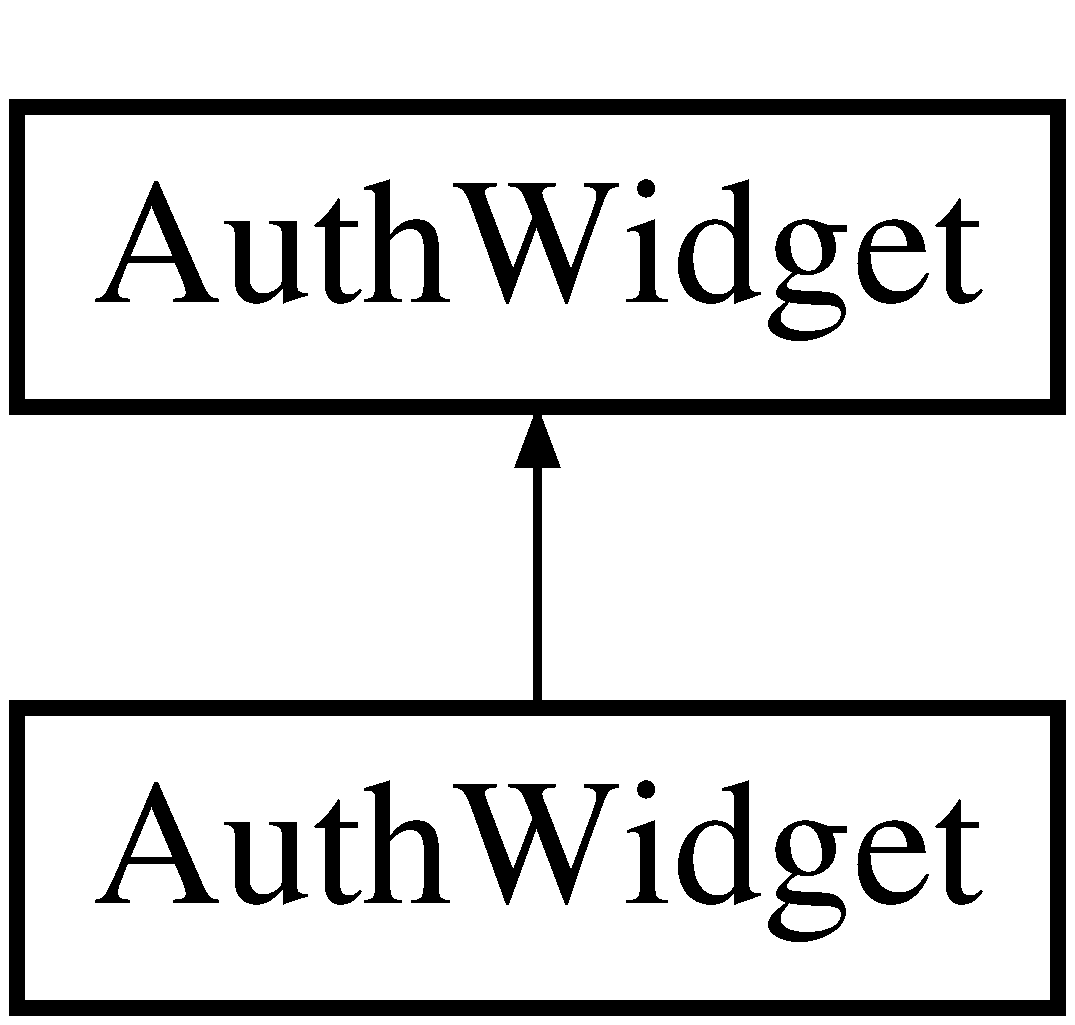
\includegraphics[height=2.000000cm]{class_auth_widget}
\end{center}
\end{figure}
\subsection*{Public Member Functions}
\begin{DoxyCompactItemize}
\item 
\hyperlink{class_auth_widget_a16b0f0ad98e79aa40992cfaa9a00cfde}{Auth\+Widget} (\hyperlink{class_session}{Session} \&session)
\item 
virtual Wt\+::\+W\+Widget $\ast$ \hyperlink{class_auth_widget_abfa295703272e72a5d57dd736cc9f329}{create\+Registration\+View} (const Wt\+::\+Auth\+::\+Identity \&id)
\end{DoxyCompactItemize}
\subsection*{Private Attributes}
\begin{DoxyCompactItemize}
\item 
\hyperlink{class_session}{Session} \& \hyperlink{class_auth_widget_a9c1a0d3bf5d59ec8f0f6c7672e37224c}{session\+\_\+}
\end{DoxyCompactItemize}


\subsection{Constructor \& Destructor Documentation}
\mbox{\Hypertarget{class_auth_widget_a16b0f0ad98e79aa40992cfaa9a00cfde}\label{class_auth_widget_a16b0f0ad98e79aa40992cfaa9a00cfde}} 
\index{Auth\+Widget@{Auth\+Widget}!Auth\+Widget@{Auth\+Widget}}
\index{Auth\+Widget@{Auth\+Widget}!Auth\+Widget@{Auth\+Widget}}
\subsubsection{\texorpdfstring{Auth\+Widget()}{AuthWidget()}}
{\footnotesize\ttfamily Auth\+Widget\+::\+Auth\+Widget (\begin{DoxyParamCaption}\item[{\hyperlink{class_session}{Session} \&}]{session }\end{DoxyParamCaption})}



\subsection{Member Function Documentation}
\mbox{\Hypertarget{class_auth_widget_abfa295703272e72a5d57dd736cc9f329}\label{class_auth_widget_abfa295703272e72a5d57dd736cc9f329}} 
\index{Auth\+Widget@{Auth\+Widget}!create\+Registration\+View@{create\+Registration\+View}}
\index{create\+Registration\+View@{create\+Registration\+View}!Auth\+Widget@{Auth\+Widget}}
\subsubsection{\texorpdfstring{create\+Registration\+View()}{createRegistrationView()}}
{\footnotesize\ttfamily Wt\+::\+W\+Widget $\ast$ Auth\+Widget\+::create\+Registration\+View (\begin{DoxyParamCaption}\item[{const Wt\+::\+Auth\+::\+Identity \&}]{id }\end{DoxyParamCaption})\hspace{0.3cm}{\ttfamily [virtual]}}



\subsection{Member Data Documentation}
\mbox{\Hypertarget{class_auth_widget_a9c1a0d3bf5d59ec8f0f6c7672e37224c}\label{class_auth_widget_a9c1a0d3bf5d59ec8f0f6c7672e37224c}} 
\index{Auth\+Widget@{Auth\+Widget}!session\+\_\+@{session\+\_\+}}
\index{session\+\_\+@{session\+\_\+}!Auth\+Widget@{Auth\+Widget}}
\subsubsection{\texorpdfstring{session\+\_\+}{session\_}}
{\footnotesize\ttfamily \hyperlink{class_session}{Session}\& Auth\+Widget\+::session\+\_\+\hspace{0.3cm}{\ttfamily [private]}}



The documentation for this class was generated from the following files\+:\begin{DoxyCompactItemize}
\item 
\hyperlink{_auth_widget_8h}{Auth\+Widget.\+h}\item 
\hyperlink{_auth_widget_8_c}{Auth\+Widget.\+C}\end{DoxyCompactItemize}

\hypertarget{class_bridge}{}\section{Bridge Class Reference}
\label{class_bridge}\index{Bridge@{Bridge}}


{\ttfamily \#include $<$Bridge.\+h$>$}

\subsection*{Public Member Functions}
\begin{DoxyCompactItemize}
\item 
\hyperlink{class_bridge_a275f54dafc95c9b5bbaba5e904c4fa9a}{Bridge} ()
\item 
\hyperlink{class_bridge_a812b325fbb4f4b589e68f11f443a7ee4}{$\sim$\+Bridge} ()
\item 
std\+::string \hyperlink{class_bridge_a1f078fc27ba8f0fe400f78f5178355a1}{get\+Bridge\+Name} ()
\item 
std\+::string \hyperlink{class_bridge_a9c807b40340f2469ffad6a8e48bfee73}{get\+Location} ()
\item 
std\+::string \hyperlink{class_bridge_a8d0ebdced1997f8846ade31234a6ea85}{get\+Ip\+Address} ()
\item 
std\+::string \hyperlink{class_bridge_acd998fba0043a2a2adeccd1a5f35bb79}{get\+Host\+Name} ()
\item 
std\+::string \hyperlink{class_bridge_ab74c5db6065cedb1aabb0a6a3775900a}{get\+User\+Id} ()
\item 
bool \hyperlink{class_bridge_a5286a8d45ce04a058c2e15730ee47b7b}{get\+Registered} ()
\item 
int \hyperlink{class_bridge_ac2ec6b055bffee5f813b1f9b70ab086b}{get\+Port\+Number} ()
\item 
void \hyperlink{class_bridge_aa4ddd6d8f8ba9d86bc5f92fda19cc66c}{set\+Bridge\+Name} (std\+::string new\+Name)
\item 
void \hyperlink{class_bridge_a23bd543d54d8b90abfa1b441f3a526ca}{set\+Location} (std\+::string new\+Location)
\item 
void \hyperlink{class_bridge_aa4fd7375d4b6092ca8bbee093dcc1a27}{set\+Ip\+Address} (std\+::string new\+Ip\+Address)
\item 
void \hyperlink{class_bridge_a1a5adca21bbdcdfe78fdd1e2f925d8c2}{set\+Host\+Name} (std\+::string new\+Host\+Name)
\item 
void \hyperlink{class_bridge_a2a68458da56a25afbbe4a8a108eb2f01}{set\+User\+Id} (std\+::string new\+User\+Id)
\item 
void \hyperlink{class_bridge_ac912eac357647d47bc87052da93c45e9}{set\+Registered} (bool new\+Registered)
\item 
void \hyperlink{class_bridge_a0acefccf95c0bf57465241ffe9618491}{set\+Port\+Number} (int new\+Port\+Number)
\item 
{\footnotesize template$<$class Action $>$ }\\void \hyperlink{class_bridge_a20b4d278bc879a5c647e106e03fa1cdc}{persist} (Action \&a)
\end{DoxyCompactItemize}
\subsection*{Public Attributes}
\begin{DoxyCompactItemize}
\item 
Wt\+::\+Dbo\+::collection$<$ Wt\+::\+Dbo\+::ptr$<$ \hyperlink{class_light}{Light} $>$ $>$ \hyperlink{class_bridge_ad2dbc05744f877c628f08ddadb84b035}{lights}
\item 
Wt\+::\+Dbo\+::collection$<$ Wt\+::\+Dbo\+::ptr$<$ \hyperlink{class_user}{User} $>$ $>$ \hyperlink{class_bridge_a84dbab519260e2e4edd8d40803b1ceec}{users}
\end{DoxyCompactItemize}
\subsection*{Private Attributes}
\begin{DoxyCompactItemize}
\item 
std\+::string \hyperlink{class_bridge_ac51c80c843b4df25faf5fa426e89811f}{bridge\+Name}
\item 
std\+::string \hyperlink{class_bridge_a04f9fec6433cadffde5fda71a004af96}{location}
\item 
std\+::string \hyperlink{class_bridge_a7e277fedd8e5d755f58c02a0f1c2bf80}{ip\+Address}
\item 
std\+::string \hyperlink{class_bridge_a6a1ca8cc945fcd364e8147188930b304}{host\+Name}
\item 
std\+::string \hyperlink{class_bridge_a99b5742c2e826c016d6e1ed2fdb2f542}{user\+Id}
\item 
bool \hyperlink{class_bridge_aad587c8a2b91ebf99d45ad9960409041}{registered}
\item 
int \hyperlink{class_bridge_af3ffbbc8063a22a9562600a098ac9109}{port\+Number}
\end{DoxyCompactItemize}


\subsection{Constructor \& Destructor Documentation}
\mbox{\Hypertarget{class_bridge_a275f54dafc95c9b5bbaba5e904c4fa9a}\label{class_bridge_a275f54dafc95c9b5bbaba5e904c4fa9a}} 
\index{Bridge@{Bridge}!Bridge@{Bridge}}
\index{Bridge@{Bridge}!Bridge@{Bridge}}
\subsubsection{\texorpdfstring{Bridge()}{Bridge()}}
{\footnotesize\ttfamily Bridge\+::\+Bridge (\begin{DoxyParamCaption}{ }\end{DoxyParamCaption})\hspace{0.3cm}{\ttfamily [inline]}}

\mbox{\Hypertarget{class_bridge_a812b325fbb4f4b589e68f11f443a7ee4}\label{class_bridge_a812b325fbb4f4b589e68f11f443a7ee4}} 
\index{Bridge@{Bridge}!````~Bridge@{$\sim$\+Bridge}}
\index{````~Bridge@{$\sim$\+Bridge}!Bridge@{Bridge}}
\subsubsection{\texorpdfstring{$\sim$\+Bridge()}{~Bridge()}}
{\footnotesize\ttfamily Bridge\+::$\sim$\+Bridge (\begin{DoxyParamCaption}{ }\end{DoxyParamCaption})\hspace{0.3cm}{\ttfamily [inline]}}



\subsection{Member Function Documentation}
\mbox{\Hypertarget{class_bridge_a1f078fc27ba8f0fe400f78f5178355a1}\label{class_bridge_a1f078fc27ba8f0fe400f78f5178355a1}} 
\index{Bridge@{Bridge}!get\+Bridge\+Name@{get\+Bridge\+Name}}
\index{get\+Bridge\+Name@{get\+Bridge\+Name}!Bridge@{Bridge}}
\subsubsection{\texorpdfstring{get\+Bridge\+Name()}{getBridgeName()}}
{\footnotesize\ttfamily std\+::string Bridge\+::get\+Bridge\+Name (\begin{DoxyParamCaption}{ }\end{DoxyParamCaption})\hspace{0.3cm}{\ttfamily [inline]}}

\mbox{\Hypertarget{class_bridge_acd998fba0043a2a2adeccd1a5f35bb79}\label{class_bridge_acd998fba0043a2a2adeccd1a5f35bb79}} 
\index{Bridge@{Bridge}!get\+Host\+Name@{get\+Host\+Name}}
\index{get\+Host\+Name@{get\+Host\+Name}!Bridge@{Bridge}}
\subsubsection{\texorpdfstring{get\+Host\+Name()}{getHostName()}}
{\footnotesize\ttfamily std\+::string Bridge\+::get\+Host\+Name (\begin{DoxyParamCaption}{ }\end{DoxyParamCaption})\hspace{0.3cm}{\ttfamily [inline]}}

\mbox{\Hypertarget{class_bridge_a8d0ebdced1997f8846ade31234a6ea85}\label{class_bridge_a8d0ebdced1997f8846ade31234a6ea85}} 
\index{Bridge@{Bridge}!get\+Ip\+Address@{get\+Ip\+Address}}
\index{get\+Ip\+Address@{get\+Ip\+Address}!Bridge@{Bridge}}
\subsubsection{\texorpdfstring{get\+Ip\+Address()}{getIpAddress()}}
{\footnotesize\ttfamily std\+::string Bridge\+::get\+Ip\+Address (\begin{DoxyParamCaption}{ }\end{DoxyParamCaption})\hspace{0.3cm}{\ttfamily [inline]}}

\mbox{\Hypertarget{class_bridge_a9c807b40340f2469ffad6a8e48bfee73}\label{class_bridge_a9c807b40340f2469ffad6a8e48bfee73}} 
\index{Bridge@{Bridge}!get\+Location@{get\+Location}}
\index{get\+Location@{get\+Location}!Bridge@{Bridge}}
\subsubsection{\texorpdfstring{get\+Location()}{getLocation()}}
{\footnotesize\ttfamily std\+::string Bridge\+::get\+Location (\begin{DoxyParamCaption}{ }\end{DoxyParamCaption})\hspace{0.3cm}{\ttfamily [inline]}}

\mbox{\Hypertarget{class_bridge_ac2ec6b055bffee5f813b1f9b70ab086b}\label{class_bridge_ac2ec6b055bffee5f813b1f9b70ab086b}} 
\index{Bridge@{Bridge}!get\+Port\+Number@{get\+Port\+Number}}
\index{get\+Port\+Number@{get\+Port\+Number}!Bridge@{Bridge}}
\subsubsection{\texorpdfstring{get\+Port\+Number()}{getPortNumber()}}
{\footnotesize\ttfamily int Bridge\+::get\+Port\+Number (\begin{DoxyParamCaption}{ }\end{DoxyParamCaption})\hspace{0.3cm}{\ttfamily [inline]}}

\mbox{\Hypertarget{class_bridge_a5286a8d45ce04a058c2e15730ee47b7b}\label{class_bridge_a5286a8d45ce04a058c2e15730ee47b7b}} 
\index{Bridge@{Bridge}!get\+Registered@{get\+Registered}}
\index{get\+Registered@{get\+Registered}!Bridge@{Bridge}}
\subsubsection{\texorpdfstring{get\+Registered()}{getRegistered()}}
{\footnotesize\ttfamily bool Bridge\+::get\+Registered (\begin{DoxyParamCaption}{ }\end{DoxyParamCaption})\hspace{0.3cm}{\ttfamily [inline]}}

\mbox{\Hypertarget{class_bridge_ab74c5db6065cedb1aabb0a6a3775900a}\label{class_bridge_ab74c5db6065cedb1aabb0a6a3775900a}} 
\index{Bridge@{Bridge}!get\+User\+Id@{get\+User\+Id}}
\index{get\+User\+Id@{get\+User\+Id}!Bridge@{Bridge}}
\subsubsection{\texorpdfstring{get\+User\+Id()}{getUserId()}}
{\footnotesize\ttfamily std\+::string Bridge\+::get\+User\+Id (\begin{DoxyParamCaption}{ }\end{DoxyParamCaption})\hspace{0.3cm}{\ttfamily [inline]}}

\mbox{\Hypertarget{class_bridge_a20b4d278bc879a5c647e106e03fa1cdc}\label{class_bridge_a20b4d278bc879a5c647e106e03fa1cdc}} 
\index{Bridge@{Bridge}!persist@{persist}}
\index{persist@{persist}!Bridge@{Bridge}}
\subsubsection{\texorpdfstring{persist()}{persist()}}
{\footnotesize\ttfamily template$<$class Action $>$ \\
void Bridge\+::persist (\begin{DoxyParamCaption}\item[{Action \&}]{a }\end{DoxyParamCaption})\hspace{0.3cm}{\ttfamily [inline]}}

\mbox{\Hypertarget{class_bridge_aa4ddd6d8f8ba9d86bc5f92fda19cc66c}\label{class_bridge_aa4ddd6d8f8ba9d86bc5f92fda19cc66c}} 
\index{Bridge@{Bridge}!set\+Bridge\+Name@{set\+Bridge\+Name}}
\index{set\+Bridge\+Name@{set\+Bridge\+Name}!Bridge@{Bridge}}
\subsubsection{\texorpdfstring{set\+Bridge\+Name()}{setBridgeName()}}
{\footnotesize\ttfamily void Bridge\+::set\+Bridge\+Name (\begin{DoxyParamCaption}\item[{std\+::string}]{new\+Name }\end{DoxyParamCaption})\hspace{0.3cm}{\ttfamily [inline]}}

\mbox{\Hypertarget{class_bridge_a1a5adca21bbdcdfe78fdd1e2f925d8c2}\label{class_bridge_a1a5adca21bbdcdfe78fdd1e2f925d8c2}} 
\index{Bridge@{Bridge}!set\+Host\+Name@{set\+Host\+Name}}
\index{set\+Host\+Name@{set\+Host\+Name}!Bridge@{Bridge}}
\subsubsection{\texorpdfstring{set\+Host\+Name()}{setHostName()}}
{\footnotesize\ttfamily void Bridge\+::set\+Host\+Name (\begin{DoxyParamCaption}\item[{std\+::string}]{new\+Host\+Name }\end{DoxyParamCaption})\hspace{0.3cm}{\ttfamily [inline]}}

\mbox{\Hypertarget{class_bridge_aa4fd7375d4b6092ca8bbee093dcc1a27}\label{class_bridge_aa4fd7375d4b6092ca8bbee093dcc1a27}} 
\index{Bridge@{Bridge}!set\+Ip\+Address@{set\+Ip\+Address}}
\index{set\+Ip\+Address@{set\+Ip\+Address}!Bridge@{Bridge}}
\subsubsection{\texorpdfstring{set\+Ip\+Address()}{setIpAddress()}}
{\footnotesize\ttfamily void Bridge\+::set\+Ip\+Address (\begin{DoxyParamCaption}\item[{std\+::string}]{new\+Ip\+Address }\end{DoxyParamCaption})\hspace{0.3cm}{\ttfamily [inline]}}

\mbox{\Hypertarget{class_bridge_a23bd543d54d8b90abfa1b441f3a526ca}\label{class_bridge_a23bd543d54d8b90abfa1b441f3a526ca}} 
\index{Bridge@{Bridge}!set\+Location@{set\+Location}}
\index{set\+Location@{set\+Location}!Bridge@{Bridge}}
\subsubsection{\texorpdfstring{set\+Location()}{setLocation()}}
{\footnotesize\ttfamily void Bridge\+::set\+Location (\begin{DoxyParamCaption}\item[{std\+::string}]{new\+Location }\end{DoxyParamCaption})\hspace{0.3cm}{\ttfamily [inline]}}

\mbox{\Hypertarget{class_bridge_a0acefccf95c0bf57465241ffe9618491}\label{class_bridge_a0acefccf95c0bf57465241ffe9618491}} 
\index{Bridge@{Bridge}!set\+Port\+Number@{set\+Port\+Number}}
\index{set\+Port\+Number@{set\+Port\+Number}!Bridge@{Bridge}}
\subsubsection{\texorpdfstring{set\+Port\+Number()}{setPortNumber()}}
{\footnotesize\ttfamily void Bridge\+::set\+Port\+Number (\begin{DoxyParamCaption}\item[{int}]{new\+Port\+Number }\end{DoxyParamCaption})\hspace{0.3cm}{\ttfamily [inline]}}

\mbox{\Hypertarget{class_bridge_ac912eac357647d47bc87052da93c45e9}\label{class_bridge_ac912eac357647d47bc87052da93c45e9}} 
\index{Bridge@{Bridge}!set\+Registered@{set\+Registered}}
\index{set\+Registered@{set\+Registered}!Bridge@{Bridge}}
\subsubsection{\texorpdfstring{set\+Registered()}{setRegistered()}}
{\footnotesize\ttfamily void Bridge\+::set\+Registered (\begin{DoxyParamCaption}\item[{bool}]{new\+Registered }\end{DoxyParamCaption})\hspace{0.3cm}{\ttfamily [inline]}}

\mbox{\Hypertarget{class_bridge_a2a68458da56a25afbbe4a8a108eb2f01}\label{class_bridge_a2a68458da56a25afbbe4a8a108eb2f01}} 
\index{Bridge@{Bridge}!set\+User\+Id@{set\+User\+Id}}
\index{set\+User\+Id@{set\+User\+Id}!Bridge@{Bridge}}
\subsubsection{\texorpdfstring{set\+User\+Id()}{setUserId()}}
{\footnotesize\ttfamily void Bridge\+::set\+User\+Id (\begin{DoxyParamCaption}\item[{std\+::string}]{new\+User\+Id }\end{DoxyParamCaption})\hspace{0.3cm}{\ttfamily [inline]}}



\subsection{Member Data Documentation}
\mbox{\Hypertarget{class_bridge_ac51c80c843b4df25faf5fa426e89811f}\label{class_bridge_ac51c80c843b4df25faf5fa426e89811f}} 
\index{Bridge@{Bridge}!bridge\+Name@{bridge\+Name}}
\index{bridge\+Name@{bridge\+Name}!Bridge@{Bridge}}
\subsubsection{\texorpdfstring{bridge\+Name}{bridgeName}}
{\footnotesize\ttfamily std\+::string Bridge\+::bridge\+Name\hspace{0.3cm}{\ttfamily [private]}}

\mbox{\Hypertarget{class_bridge_a6a1ca8cc945fcd364e8147188930b304}\label{class_bridge_a6a1ca8cc945fcd364e8147188930b304}} 
\index{Bridge@{Bridge}!host\+Name@{host\+Name}}
\index{host\+Name@{host\+Name}!Bridge@{Bridge}}
\subsubsection{\texorpdfstring{host\+Name}{hostName}}
{\footnotesize\ttfamily std\+::string Bridge\+::host\+Name\hspace{0.3cm}{\ttfamily [private]}}

\mbox{\Hypertarget{class_bridge_a7e277fedd8e5d755f58c02a0f1c2bf80}\label{class_bridge_a7e277fedd8e5d755f58c02a0f1c2bf80}} 
\index{Bridge@{Bridge}!ip\+Address@{ip\+Address}}
\index{ip\+Address@{ip\+Address}!Bridge@{Bridge}}
\subsubsection{\texorpdfstring{ip\+Address}{ipAddress}}
{\footnotesize\ttfamily std\+::string Bridge\+::ip\+Address\hspace{0.3cm}{\ttfamily [private]}}

\mbox{\Hypertarget{class_bridge_ad2dbc05744f877c628f08ddadb84b035}\label{class_bridge_ad2dbc05744f877c628f08ddadb84b035}} 
\index{Bridge@{Bridge}!lights@{lights}}
\index{lights@{lights}!Bridge@{Bridge}}
\subsubsection{\texorpdfstring{lights}{lights}}
{\footnotesize\ttfamily Wt\+::\+Dbo\+::collection$<$Wt\+::\+Dbo\+::ptr$<$\hyperlink{class_light}{Light}$>$ $>$ Bridge\+::lights}

\mbox{\Hypertarget{class_bridge_a04f9fec6433cadffde5fda71a004af96}\label{class_bridge_a04f9fec6433cadffde5fda71a004af96}} 
\index{Bridge@{Bridge}!location@{location}}
\index{location@{location}!Bridge@{Bridge}}
\subsubsection{\texorpdfstring{location}{location}}
{\footnotesize\ttfamily std\+::string Bridge\+::location\hspace{0.3cm}{\ttfamily [private]}}

\mbox{\Hypertarget{class_bridge_af3ffbbc8063a22a9562600a098ac9109}\label{class_bridge_af3ffbbc8063a22a9562600a098ac9109}} 
\index{Bridge@{Bridge}!port\+Number@{port\+Number}}
\index{port\+Number@{port\+Number}!Bridge@{Bridge}}
\subsubsection{\texorpdfstring{port\+Number}{portNumber}}
{\footnotesize\ttfamily int Bridge\+::port\+Number\hspace{0.3cm}{\ttfamily [private]}}

\mbox{\Hypertarget{class_bridge_aad587c8a2b91ebf99d45ad9960409041}\label{class_bridge_aad587c8a2b91ebf99d45ad9960409041}} 
\index{Bridge@{Bridge}!registered@{registered}}
\index{registered@{registered}!Bridge@{Bridge}}
\subsubsection{\texorpdfstring{registered}{registered}}
{\footnotesize\ttfamily bool Bridge\+::registered\hspace{0.3cm}{\ttfamily [private]}}

\mbox{\Hypertarget{class_bridge_a99b5742c2e826c016d6e1ed2fdb2f542}\label{class_bridge_a99b5742c2e826c016d6e1ed2fdb2f542}} 
\index{Bridge@{Bridge}!user\+Id@{user\+Id}}
\index{user\+Id@{user\+Id}!Bridge@{Bridge}}
\subsubsection{\texorpdfstring{user\+Id}{userId}}
{\footnotesize\ttfamily std\+::string Bridge\+::user\+Id\hspace{0.3cm}{\ttfamily [private]}}

\mbox{\Hypertarget{class_bridge_a84dbab519260e2e4edd8d40803b1ceec}\label{class_bridge_a84dbab519260e2e4edd8d40803b1ceec}} 
\index{Bridge@{Bridge}!users@{users}}
\index{users@{users}!Bridge@{Bridge}}
\subsubsection{\texorpdfstring{users}{users}}
{\footnotesize\ttfamily Wt\+::\+Dbo\+::collection$<$Wt\+::\+Dbo\+::ptr$<$\hyperlink{class_user}{User}$>$ $>$ Bridge\+::users}



The documentation for this class was generated from the following file\+:\begin{DoxyCompactItemize}
\item 
\hyperlink{_bridge_8h}{Bridge.\+h}\end{DoxyCompactItemize}

\hypertarget{class_bridge_control_widget}{}\section{Bridge\+Control\+Widget Class Reference}
\label{class_bridge_control_widget}\index{Bridge\+Control\+Widget@{Bridge\+Control\+Widget}}


{\ttfamily \#include $<$Bridge\+Control.\+h$>$}

Inheritance diagram for Bridge\+Control\+Widget\+:\begin{figure}[H]
\begin{center}
\leavevmode
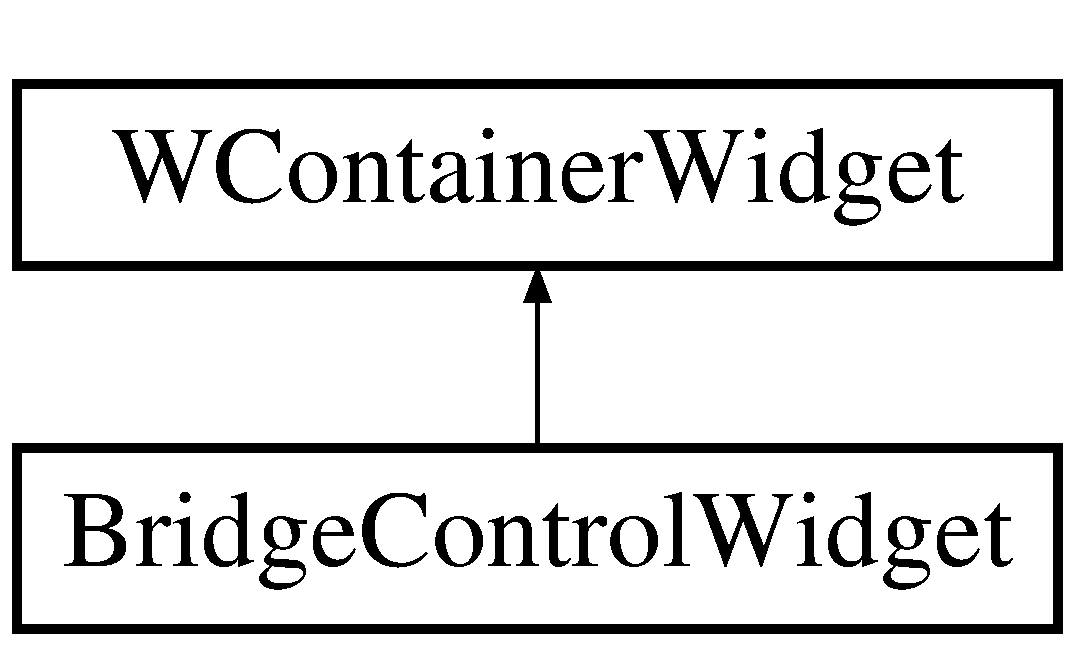
\includegraphics[height=2.000000cm]{class_bridge_control_widget}
\end{center}
\end{figure}
\subsection*{Public Member Functions}
\begin{DoxyCompactItemize}
\item 
\hyperlink{class_bridge_control_widget_af09e7c2a5993cd307c99ad8c9f964542}{Bridge\+Control\+Widget} (\hyperlink{class_session}{Session} $\ast$session, W\+Container\+Widget $\ast$parent)
\item 
void \hyperlink{class_bridge_control_widget_af8533ce9fe9765ff317d9215fb6aa4da}{update} ()
\end{DoxyCompactItemize}
\subsection*{Private Member Functions}
\begin{DoxyCompactItemize}
\item 
void \hyperlink{class_bridge_control_widget_a894337cd809042fcae667a8caa3f9451}{handle\+Http\+Response} (boost\+::system\+::error\+\_\+code err, const Wt\+::\+Http\+::\+Message \&response)
\item 
Wt\+::\+Http\+::\+Client $\ast$ \hyperlink{class_bridge_control_widget_aaab68c6bb33f44c2edeea7942e190ec6}{connect} ()
\item 
void \hyperlink{class_bridge_control_widget_a23d4fac71d031ec1c4783af139962754}{register\+Bridge} ()
\item 
void \hyperlink{class_bridge_control_widget_ae1204ba0a72cf3a6719fda099532f939}{show\+Lights} ()
\item 
void \hyperlink{class_bridge_control_widget_a5cabafd79c446bbdd5a75a4eee9b316a}{test} ()
\end{DoxyCompactItemize}
\subsection*{Private Attributes}
\begin{DoxyCompactItemize}
\item 
\hyperlink{class_session}{Session} $\ast$ \hyperlink{class_bridge_control_widget_a8515acd4aba4adfc0ca0f303cc774714}{session\+\_\+}
\item 
Wt\+::\+W\+Text $\ast$ \hyperlink{class_bridge_control_widget_aade9df1dc99afdac9fe1aca212957556}{user\+\_\+}
\item 
Wt\+::\+W\+Text $\ast$ \hyperlink{class_bridge_control_widget_a0976b686d1bee46834e28b70220a9bbc}{ip\+\_\+}
\item 
Wt\+::\+W\+Line\+Edit $\ast$ \hyperlink{class_bridge_control_widget_a853916f1753968ac0a897ebaa5c0cbcc}{ip\+Edit\+\_\+}
\item 
Wt\+::\+W\+Text $\ast$ \hyperlink{class_bridge_control_widget_a0eae40d451b31b92112ec212516372cb}{port\+\_\+}
\item 
Wt\+::\+W\+Line\+Edit $\ast$ \hyperlink{class_bridge_control_widget_a41af1fb420ff88d4e4d3981b3c6e5c04}{port\+Edit\+\_\+}
\item 
Wt\+::\+W\+Text $\ast$ \hyperlink{class_bridge_control_widget_ad3a9a0bd678c760b74ef61b5c78bbea3}{location\+\_\+}
\item 
Wt\+::\+W\+Line\+Edit $\ast$ \hyperlink{class_bridge_control_widget_a69f59affca4084dd6be95e637e4d0a37}{location\+Edit\+\_\+}
\item 
Wt\+::\+W\+Line\+Edit $\ast$ \hyperlink{class_bridge_control_widget_a34ffd7c6178a84184d43b1f403fd1945}{name\+\_\+}
\item 
Wt\+::\+W\+Push\+Button $\ast$ \hyperlink{class_bridge_control_widget_ae44e24e9f180d7d8727a5989467a627e}{button}
\item 
Wt\+::\+W\+Text $\ast$ \hyperlink{class_bridge_control_widget_a3a1af1bc24a550a4bff633f62cb54b00}{error\+Text\+\_\+}
\item 
Wt\+::\+W\+Text $\ast$ \hyperlink{class_bridge_control_widget_a8fc1ea20843b3715ddbf72ef4aa84c6c}{confirm\+\_\+}
\item 
std\+::string \hyperlink{class_bridge_control_widget_ac195eb9bda89539ad76dcb68c183d7d3}{username}
\item 
std\+::string \hyperlink{class_bridge_control_widget_a0d2312d2fd67c2ed6a285d6c2e336d29}{ip}
\item 
std\+::string \hyperlink{class_bridge_control_widget_a1c8a761d43d554385f1d5416c611665c}{port}
\item 
Wt\+::\+W\+Sound $\ast$ \hyperlink{class_bridge_control_widget_a95671fff1cc255ba4d5eaaab4c1a8277}{message\+Received\+\_\+}
\end{DoxyCompactItemize}


\subsection{Constructor \& Destructor Documentation}
\mbox{\Hypertarget{class_bridge_control_widget_af09e7c2a5993cd307c99ad8c9f964542}\label{class_bridge_control_widget_af09e7c2a5993cd307c99ad8c9f964542}} 
\index{Bridge\+Control\+Widget@{Bridge\+Control\+Widget}!Bridge\+Control\+Widget@{Bridge\+Control\+Widget}}
\index{Bridge\+Control\+Widget@{Bridge\+Control\+Widget}!Bridge\+Control\+Widget@{Bridge\+Control\+Widget}}
\subsubsection{\texorpdfstring{Bridge\+Control\+Widget()}{BridgeControlWidget()}}
{\footnotesize\ttfamily Bridge\+Control\+Widget\+::\+Bridge\+Control\+Widget (\begin{DoxyParamCaption}\item[{\hyperlink{class_session}{Session} $\ast$}]{session,  }\item[{W\+Container\+Widget $\ast$}]{parent }\end{DoxyParamCaption})}



\subsection{Member Function Documentation}
\mbox{\Hypertarget{class_bridge_control_widget_aaab68c6bb33f44c2edeea7942e190ec6}\label{class_bridge_control_widget_aaab68c6bb33f44c2edeea7942e190ec6}} 
\index{Bridge\+Control\+Widget@{Bridge\+Control\+Widget}!connect@{connect}}
\index{connect@{connect}!Bridge\+Control\+Widget@{Bridge\+Control\+Widget}}
\subsubsection{\texorpdfstring{connect()}{connect()}}
{\footnotesize\ttfamily Http\+::\+Client $\ast$ Bridge\+Control\+Widget\+::connect (\begin{DoxyParamCaption}{ }\end{DoxyParamCaption})\hspace{0.3cm}{\ttfamily [private]}}

\mbox{\Hypertarget{class_bridge_control_widget_a894337cd809042fcae667a8caa3f9451}\label{class_bridge_control_widget_a894337cd809042fcae667a8caa3f9451}} 
\index{Bridge\+Control\+Widget@{Bridge\+Control\+Widget}!handle\+Http\+Response@{handle\+Http\+Response}}
\index{handle\+Http\+Response@{handle\+Http\+Response}!Bridge\+Control\+Widget@{Bridge\+Control\+Widget}}
\subsubsection{\texorpdfstring{handle\+Http\+Response()}{handleHttpResponse()}}
{\footnotesize\ttfamily void Bridge\+Control\+Widget\+::handle\+Http\+Response (\begin{DoxyParamCaption}\item[{boost\+::system\+::error\+\_\+code}]{err,  }\item[{const Wt\+::\+Http\+::\+Message \&}]{response }\end{DoxyParamCaption})\hspace{0.3cm}{\ttfamily [private]}}

\mbox{\Hypertarget{class_bridge_control_widget_a23d4fac71d031ec1c4783af139962754}\label{class_bridge_control_widget_a23d4fac71d031ec1c4783af139962754}} 
\index{Bridge\+Control\+Widget@{Bridge\+Control\+Widget}!register\+Bridge@{register\+Bridge}}
\index{register\+Bridge@{register\+Bridge}!Bridge\+Control\+Widget@{Bridge\+Control\+Widget}}
\subsubsection{\texorpdfstring{register\+Bridge()}{registerBridge()}}
{\footnotesize\ttfamily void Bridge\+Control\+Widget\+::register\+Bridge (\begin{DoxyParamCaption}{ }\end{DoxyParamCaption})\hspace{0.3cm}{\ttfamily [private]}}

\mbox{\Hypertarget{class_bridge_control_widget_ae1204ba0a72cf3a6719fda099532f939}\label{class_bridge_control_widget_ae1204ba0a72cf3a6719fda099532f939}} 
\index{Bridge\+Control\+Widget@{Bridge\+Control\+Widget}!show\+Lights@{show\+Lights}}
\index{show\+Lights@{show\+Lights}!Bridge\+Control\+Widget@{Bridge\+Control\+Widget}}
\subsubsection{\texorpdfstring{show\+Lights()}{showLights()}}
{\footnotesize\ttfamily void Bridge\+Control\+Widget\+::show\+Lights (\begin{DoxyParamCaption}{ }\end{DoxyParamCaption})\hspace{0.3cm}{\ttfamily [private]}}

\mbox{\Hypertarget{class_bridge_control_widget_a5cabafd79c446bbdd5a75a4eee9b316a}\label{class_bridge_control_widget_a5cabafd79c446bbdd5a75a4eee9b316a}} 
\index{Bridge\+Control\+Widget@{Bridge\+Control\+Widget}!test@{test}}
\index{test@{test}!Bridge\+Control\+Widget@{Bridge\+Control\+Widget}}
\subsubsection{\texorpdfstring{test()}{test()}}
{\footnotesize\ttfamily void Bridge\+Control\+Widget\+::test (\begin{DoxyParamCaption}{ }\end{DoxyParamCaption})\hspace{0.3cm}{\ttfamily [private]}}

\mbox{\Hypertarget{class_bridge_control_widget_af8533ce9fe9765ff317d9215fb6aa4da}\label{class_bridge_control_widget_af8533ce9fe9765ff317d9215fb6aa4da}} 
\index{Bridge\+Control\+Widget@{Bridge\+Control\+Widget}!update@{update}}
\index{update@{update}!Bridge\+Control\+Widget@{Bridge\+Control\+Widget}}
\subsubsection{\texorpdfstring{update()}{update()}}
{\footnotesize\ttfamily void Bridge\+Control\+Widget\+::update (\begin{DoxyParamCaption}{ }\end{DoxyParamCaption})}



\subsection{Member Data Documentation}
\mbox{\Hypertarget{class_bridge_control_widget_ae44e24e9f180d7d8727a5989467a627e}\label{class_bridge_control_widget_ae44e24e9f180d7d8727a5989467a627e}} 
\index{Bridge\+Control\+Widget@{Bridge\+Control\+Widget}!button@{button}}
\index{button@{button}!Bridge\+Control\+Widget@{Bridge\+Control\+Widget}}
\subsubsection{\texorpdfstring{button}{button}}
{\footnotesize\ttfamily Wt\+::\+W\+Push\+Button$\ast$ Bridge\+Control\+Widget\+::button\hspace{0.3cm}{\ttfamily [private]}}

\mbox{\Hypertarget{class_bridge_control_widget_a8fc1ea20843b3715ddbf72ef4aa84c6c}\label{class_bridge_control_widget_a8fc1ea20843b3715ddbf72ef4aa84c6c}} 
\index{Bridge\+Control\+Widget@{Bridge\+Control\+Widget}!confirm\+\_\+@{confirm\+\_\+}}
\index{confirm\+\_\+@{confirm\+\_\+}!Bridge\+Control\+Widget@{Bridge\+Control\+Widget}}
\subsubsection{\texorpdfstring{confirm\+\_\+}{confirm\_}}
{\footnotesize\ttfamily Wt\+::\+W\+Text$\ast$ Bridge\+Control\+Widget\+::confirm\+\_\+\hspace{0.3cm}{\ttfamily [private]}}

\mbox{\Hypertarget{class_bridge_control_widget_a3a1af1bc24a550a4bff633f62cb54b00}\label{class_bridge_control_widget_a3a1af1bc24a550a4bff633f62cb54b00}} 
\index{Bridge\+Control\+Widget@{Bridge\+Control\+Widget}!error\+Text\+\_\+@{error\+Text\+\_\+}}
\index{error\+Text\+\_\+@{error\+Text\+\_\+}!Bridge\+Control\+Widget@{Bridge\+Control\+Widget}}
\subsubsection{\texorpdfstring{error\+Text\+\_\+}{errorText\_}}
{\footnotesize\ttfamily Wt\+::\+W\+Text$\ast$ Bridge\+Control\+Widget\+::error\+Text\+\_\+\hspace{0.3cm}{\ttfamily [private]}}

\mbox{\Hypertarget{class_bridge_control_widget_a0d2312d2fd67c2ed6a285d6c2e336d29}\label{class_bridge_control_widget_a0d2312d2fd67c2ed6a285d6c2e336d29}} 
\index{Bridge\+Control\+Widget@{Bridge\+Control\+Widget}!ip@{ip}}
\index{ip@{ip}!Bridge\+Control\+Widget@{Bridge\+Control\+Widget}}
\subsubsection{\texorpdfstring{ip}{ip}}
{\footnotesize\ttfamily std\+::string Bridge\+Control\+Widget\+::ip\hspace{0.3cm}{\ttfamily [private]}}

\mbox{\Hypertarget{class_bridge_control_widget_a0976b686d1bee46834e28b70220a9bbc}\label{class_bridge_control_widget_a0976b686d1bee46834e28b70220a9bbc}} 
\index{Bridge\+Control\+Widget@{Bridge\+Control\+Widget}!ip\+\_\+@{ip\+\_\+}}
\index{ip\+\_\+@{ip\+\_\+}!Bridge\+Control\+Widget@{Bridge\+Control\+Widget}}
\subsubsection{\texorpdfstring{ip\+\_\+}{ip\_}}
{\footnotesize\ttfamily Wt\+::\+W\+Text$\ast$ Bridge\+Control\+Widget\+::ip\+\_\+\hspace{0.3cm}{\ttfamily [private]}}

\mbox{\Hypertarget{class_bridge_control_widget_a853916f1753968ac0a897ebaa5c0cbcc}\label{class_bridge_control_widget_a853916f1753968ac0a897ebaa5c0cbcc}} 
\index{Bridge\+Control\+Widget@{Bridge\+Control\+Widget}!ip\+Edit\+\_\+@{ip\+Edit\+\_\+}}
\index{ip\+Edit\+\_\+@{ip\+Edit\+\_\+}!Bridge\+Control\+Widget@{Bridge\+Control\+Widget}}
\subsubsection{\texorpdfstring{ip\+Edit\+\_\+}{ipEdit\_}}
{\footnotesize\ttfamily Wt\+::\+W\+Line\+Edit$\ast$ Bridge\+Control\+Widget\+::ip\+Edit\+\_\+\hspace{0.3cm}{\ttfamily [private]}}

\mbox{\Hypertarget{class_bridge_control_widget_ad3a9a0bd678c760b74ef61b5c78bbea3}\label{class_bridge_control_widget_ad3a9a0bd678c760b74ef61b5c78bbea3}} 
\index{Bridge\+Control\+Widget@{Bridge\+Control\+Widget}!location\+\_\+@{location\+\_\+}}
\index{location\+\_\+@{location\+\_\+}!Bridge\+Control\+Widget@{Bridge\+Control\+Widget}}
\subsubsection{\texorpdfstring{location\+\_\+}{location\_}}
{\footnotesize\ttfamily Wt\+::\+W\+Text$\ast$ Bridge\+Control\+Widget\+::location\+\_\+\hspace{0.3cm}{\ttfamily [private]}}

\mbox{\Hypertarget{class_bridge_control_widget_a69f59affca4084dd6be95e637e4d0a37}\label{class_bridge_control_widget_a69f59affca4084dd6be95e637e4d0a37}} 
\index{Bridge\+Control\+Widget@{Bridge\+Control\+Widget}!location\+Edit\+\_\+@{location\+Edit\+\_\+}}
\index{location\+Edit\+\_\+@{location\+Edit\+\_\+}!Bridge\+Control\+Widget@{Bridge\+Control\+Widget}}
\subsubsection{\texorpdfstring{location\+Edit\+\_\+}{locationEdit\_}}
{\footnotesize\ttfamily Wt\+::\+W\+Line\+Edit$\ast$ Bridge\+Control\+Widget\+::location\+Edit\+\_\+\hspace{0.3cm}{\ttfamily [private]}}

\mbox{\Hypertarget{class_bridge_control_widget_a95671fff1cc255ba4d5eaaab4c1a8277}\label{class_bridge_control_widget_a95671fff1cc255ba4d5eaaab4c1a8277}} 
\index{Bridge\+Control\+Widget@{Bridge\+Control\+Widget}!message\+Received\+\_\+@{message\+Received\+\_\+}}
\index{message\+Received\+\_\+@{message\+Received\+\_\+}!Bridge\+Control\+Widget@{Bridge\+Control\+Widget}}
\subsubsection{\texorpdfstring{message\+Received\+\_\+}{messageReceived\_}}
{\footnotesize\ttfamily Wt\+::\+W\+Sound$\ast$ Bridge\+Control\+Widget\+::message\+Received\+\_\+\hspace{0.3cm}{\ttfamily [private]}}

\mbox{\Hypertarget{class_bridge_control_widget_a34ffd7c6178a84184d43b1f403fd1945}\label{class_bridge_control_widget_a34ffd7c6178a84184d43b1f403fd1945}} 
\index{Bridge\+Control\+Widget@{Bridge\+Control\+Widget}!name\+\_\+@{name\+\_\+}}
\index{name\+\_\+@{name\+\_\+}!Bridge\+Control\+Widget@{Bridge\+Control\+Widget}}
\subsubsection{\texorpdfstring{name\+\_\+}{name\_}}
{\footnotesize\ttfamily Wt\+::\+W\+Line\+Edit$\ast$ Bridge\+Control\+Widget\+::name\+\_\+\hspace{0.3cm}{\ttfamily [private]}}

\mbox{\Hypertarget{class_bridge_control_widget_a1c8a761d43d554385f1d5416c611665c}\label{class_bridge_control_widget_a1c8a761d43d554385f1d5416c611665c}} 
\index{Bridge\+Control\+Widget@{Bridge\+Control\+Widget}!port@{port}}
\index{port@{port}!Bridge\+Control\+Widget@{Bridge\+Control\+Widget}}
\subsubsection{\texorpdfstring{port}{port}}
{\footnotesize\ttfamily std\+::string Bridge\+Control\+Widget\+::port\hspace{0.3cm}{\ttfamily [private]}}

\mbox{\Hypertarget{class_bridge_control_widget_a0eae40d451b31b92112ec212516372cb}\label{class_bridge_control_widget_a0eae40d451b31b92112ec212516372cb}} 
\index{Bridge\+Control\+Widget@{Bridge\+Control\+Widget}!port\+\_\+@{port\+\_\+}}
\index{port\+\_\+@{port\+\_\+}!Bridge\+Control\+Widget@{Bridge\+Control\+Widget}}
\subsubsection{\texorpdfstring{port\+\_\+}{port\_}}
{\footnotesize\ttfamily Wt\+::\+W\+Text$\ast$ Bridge\+Control\+Widget\+::port\+\_\+\hspace{0.3cm}{\ttfamily [private]}}

\mbox{\Hypertarget{class_bridge_control_widget_a41af1fb420ff88d4e4d3981b3c6e5c04}\label{class_bridge_control_widget_a41af1fb420ff88d4e4d3981b3c6e5c04}} 
\index{Bridge\+Control\+Widget@{Bridge\+Control\+Widget}!port\+Edit\+\_\+@{port\+Edit\+\_\+}}
\index{port\+Edit\+\_\+@{port\+Edit\+\_\+}!Bridge\+Control\+Widget@{Bridge\+Control\+Widget}}
\subsubsection{\texorpdfstring{port\+Edit\+\_\+}{portEdit\_}}
{\footnotesize\ttfamily Wt\+::\+W\+Line\+Edit$\ast$ Bridge\+Control\+Widget\+::port\+Edit\+\_\+\hspace{0.3cm}{\ttfamily [private]}}

\mbox{\Hypertarget{class_bridge_control_widget_a8515acd4aba4adfc0ca0f303cc774714}\label{class_bridge_control_widget_a8515acd4aba4adfc0ca0f303cc774714}} 
\index{Bridge\+Control\+Widget@{Bridge\+Control\+Widget}!session\+\_\+@{session\+\_\+}}
\index{session\+\_\+@{session\+\_\+}!Bridge\+Control\+Widget@{Bridge\+Control\+Widget}}
\subsubsection{\texorpdfstring{session\+\_\+}{session\_}}
{\footnotesize\ttfamily \hyperlink{class_session}{Session}$\ast$ Bridge\+Control\+Widget\+::session\+\_\+\hspace{0.3cm}{\ttfamily [private]}}

\mbox{\Hypertarget{class_bridge_control_widget_aade9df1dc99afdac9fe1aca212957556}\label{class_bridge_control_widget_aade9df1dc99afdac9fe1aca212957556}} 
\index{Bridge\+Control\+Widget@{Bridge\+Control\+Widget}!user\+\_\+@{user\+\_\+}}
\index{user\+\_\+@{user\+\_\+}!Bridge\+Control\+Widget@{Bridge\+Control\+Widget}}
\subsubsection{\texorpdfstring{user\+\_\+}{user\_}}
{\footnotesize\ttfamily Wt\+::\+W\+Text$\ast$ Bridge\+Control\+Widget\+::user\+\_\+\hspace{0.3cm}{\ttfamily [private]}}

\mbox{\Hypertarget{class_bridge_control_widget_ac195eb9bda89539ad76dcb68c183d7d3}\label{class_bridge_control_widget_ac195eb9bda89539ad76dcb68c183d7d3}} 
\index{Bridge\+Control\+Widget@{Bridge\+Control\+Widget}!username@{username}}
\index{username@{username}!Bridge\+Control\+Widget@{Bridge\+Control\+Widget}}
\subsubsection{\texorpdfstring{username}{username}}
{\footnotesize\ttfamily std\+::string Bridge\+Control\+Widget\+::username\hspace{0.3cm}{\ttfamily [private]}}



The documentation for this class was generated from the following files\+:\begin{DoxyCompactItemize}
\item 
\hyperlink{_bridge_control_8h}{Bridge\+Control.\+h}\item 
\hyperlink{_bridge_control_8_c}{Bridge\+Control.\+C}\end{DoxyCompactItemize}

\hypertarget{class_bridge_user_ids}{}\section{Bridge\+User\+Ids Class Reference}
\label{class_bridge_user_ids}\index{Bridge\+User\+Ids@{Bridge\+User\+Ids}}


{\ttfamily \#include $<$Bridge\+User\+Ids.\+h$>$}

\subsection*{Public Member Functions}
\begin{DoxyCompactItemize}
\item 
\hyperlink{class_bridge_user_ids_ae94821f5d146bac39480c9d4c51833b9}{Bridge\+User\+Ids} ()
\item 
\hyperlink{class_bridge_user_ids_ae493577d89b03fa58a2218ec0eee466b}{Bridge\+User\+Ids} (Wt\+::\+Dbo\+::ptr$<$ \hyperlink{class_user}{User} $>$ x, Wt\+::\+Dbo\+::ptr$<$ \hyperlink{class_bridge}{Bridge} $>$ y, std\+::string id)
\item 
{\footnotesize template$<$class Action $>$ }\\void \hyperlink{class_bridge_user_ids_a8b4bf329ea12c999cca1775ef9d981cc}{persist} (Action \&a)
\end{DoxyCompactItemize}
\subsection*{Public Attributes}
\begin{DoxyCompactItemize}
\item 
std\+::string \hyperlink{class_bridge_user_ids_ae44d7688638178ed7ba299ca9687cbb5}{bridge\+User\+ID}
\item 
Wt\+::\+Dbo\+::ptr$<$ \hyperlink{class_user}{User} $>$ \hyperlink{class_bridge_user_ids_ab8cf148abfa077eb56c62576386dcffc}{user}
\item 
Wt\+::\+Dbo\+::ptr$<$ \hyperlink{class_bridge}{Bridge} $>$ \hyperlink{class_bridge_user_ids_acc206990c5f8a7faa8aa5d90c202b31a}{bridge}
\end{DoxyCompactItemize}


\subsection{Constructor \& Destructor Documentation}
\mbox{\Hypertarget{class_bridge_user_ids_ae94821f5d146bac39480c9d4c51833b9}\label{class_bridge_user_ids_ae94821f5d146bac39480c9d4c51833b9}} 
\index{Bridge\+User\+Ids@{Bridge\+User\+Ids}!Bridge\+User\+Ids@{Bridge\+User\+Ids}}
\index{Bridge\+User\+Ids@{Bridge\+User\+Ids}!Bridge\+User\+Ids@{Bridge\+User\+Ids}}
\subsubsection{\texorpdfstring{Bridge\+User\+Ids()}{BridgeUserIds()}\hspace{0.1cm}{\footnotesize\ttfamily [1/2]}}
{\footnotesize\ttfamily Bridge\+User\+Ids\+::\+Bridge\+User\+Ids (\begin{DoxyParamCaption}{ }\end{DoxyParamCaption})\hspace{0.3cm}{\ttfamily [inline]}}

\mbox{\Hypertarget{class_bridge_user_ids_ae493577d89b03fa58a2218ec0eee466b}\label{class_bridge_user_ids_ae493577d89b03fa58a2218ec0eee466b}} 
\index{Bridge\+User\+Ids@{Bridge\+User\+Ids}!Bridge\+User\+Ids@{Bridge\+User\+Ids}}
\index{Bridge\+User\+Ids@{Bridge\+User\+Ids}!Bridge\+User\+Ids@{Bridge\+User\+Ids}}
\subsubsection{\texorpdfstring{Bridge\+User\+Ids()}{BridgeUserIds()}\hspace{0.1cm}{\footnotesize\ttfamily [2/2]}}
{\footnotesize\ttfamily Bridge\+User\+Ids\+::\+Bridge\+User\+Ids (\begin{DoxyParamCaption}\item[{Wt\+::\+Dbo\+::ptr$<$ \hyperlink{class_user}{User} $>$}]{x,  }\item[{Wt\+::\+Dbo\+::ptr$<$ \hyperlink{class_bridge}{Bridge} $>$}]{y,  }\item[{std\+::string}]{id }\end{DoxyParamCaption})\hspace{0.3cm}{\ttfamily [inline]}}



\subsection{Member Function Documentation}
\mbox{\Hypertarget{class_bridge_user_ids_a8b4bf329ea12c999cca1775ef9d981cc}\label{class_bridge_user_ids_a8b4bf329ea12c999cca1775ef9d981cc}} 
\index{Bridge\+User\+Ids@{Bridge\+User\+Ids}!persist@{persist}}
\index{persist@{persist}!Bridge\+User\+Ids@{Bridge\+User\+Ids}}
\subsubsection{\texorpdfstring{persist()}{persist()}}
{\footnotesize\ttfamily template$<$class Action $>$ \\
void Bridge\+User\+Ids\+::persist (\begin{DoxyParamCaption}\item[{Action \&}]{a }\end{DoxyParamCaption})\hspace{0.3cm}{\ttfamily [inline]}}



\subsection{Member Data Documentation}
\mbox{\Hypertarget{class_bridge_user_ids_acc206990c5f8a7faa8aa5d90c202b31a}\label{class_bridge_user_ids_acc206990c5f8a7faa8aa5d90c202b31a}} 
\index{Bridge\+User\+Ids@{Bridge\+User\+Ids}!bridge@{bridge}}
\index{bridge@{bridge}!Bridge\+User\+Ids@{Bridge\+User\+Ids}}
\subsubsection{\texorpdfstring{bridge}{bridge}}
{\footnotesize\ttfamily Wt\+::\+Dbo\+::ptr$<$\hyperlink{class_bridge}{Bridge}$>$ Bridge\+User\+Ids\+::bridge}

\mbox{\Hypertarget{class_bridge_user_ids_ae44d7688638178ed7ba299ca9687cbb5}\label{class_bridge_user_ids_ae44d7688638178ed7ba299ca9687cbb5}} 
\index{Bridge\+User\+Ids@{Bridge\+User\+Ids}!bridge\+User\+ID@{bridge\+User\+ID}}
\index{bridge\+User\+ID@{bridge\+User\+ID}!Bridge\+User\+Ids@{Bridge\+User\+Ids}}
\subsubsection{\texorpdfstring{bridge\+User\+ID}{bridgeUserID}}
{\footnotesize\ttfamily std\+::string Bridge\+User\+Ids\+::bridge\+User\+ID}

\mbox{\Hypertarget{class_bridge_user_ids_ab8cf148abfa077eb56c62576386dcffc}\label{class_bridge_user_ids_ab8cf148abfa077eb56c62576386dcffc}} 
\index{Bridge\+User\+Ids@{Bridge\+User\+Ids}!user@{user}}
\index{user@{user}!Bridge\+User\+Ids@{Bridge\+User\+Ids}}
\subsubsection{\texorpdfstring{user}{user}}
{\footnotesize\ttfamily Wt\+::\+Dbo\+::ptr$<$\hyperlink{class_user}{User}$>$ Bridge\+User\+Ids\+::user}



The documentation for this class was generated from the following file\+:\begin{DoxyCompactItemize}
\item 
\hyperlink{_bridge_user_ids_8h}{Bridge\+User\+Ids.\+h}\end{DoxyCompactItemize}

\hypertarget{structdate_time}{}\section{date\+Time Struct Reference}
\label{structdate_time}\index{date\+Time@{date\+Time}}


{\ttfamily \#include $<$Scheduler\+Control.\+h$>$}

\subsection*{Public Attributes}
\begin{DoxyCompactItemize}
\item 
std\+::string \hyperlink{structdate_time_a41cb3f0c500fe4b0dcaed9eb5060a67a}{name}
\item 
char \hyperlink{structdate_time_a410eccce4f7fa017745d91b6d506aa91}{light}
\item 
int \hyperlink{structdate_time_a72fa6fd82aaa677df5fbc1111e8cec3e}{on}
\item 
int \hyperlink{structdate_time_af8b0a269b10808ee23580c36302565b9}{hue}
\item 
int \hyperlink{structdate_time_a3c1ea231c81bcb2342320b57c0cef3bd}{bri}
\item 
int \hyperlink{structdate_time_a1c206e75033573446af20f872af6ddf4}{sat}
\item 
int \hyperlink{structdate_time_ac8ace02ecb2dca3441224f4fde17b5b7}{transition}
\item 
int \hyperlink{structdate_time_a6941cd70fc3a57bca830cd1b62eb2826}{year}
\item 
int \hyperlink{structdate_time_a28451d7ddffe26ede3f38030ecc37a0b}{month}
\item 
int \hyperlink{structdate_time_a01df4912a566652a8c20a9e95e79354d}{day}
\item 
std\+::string \hyperlink{structdate_time_ab8e09ec72fd9dd7026beb7d730e1f455}{hour}
\item 
std\+::string \hyperlink{structdate_time_a8820636c9d8dee62b10129c5a5a53ea5}{min}
\item 
std\+::string \hyperlink{structdate_time_a9f45eba3d2d4d021511a66a23c5e487f}{sec}
\item 
std\+::string \hyperlink{structdate_time_af60a96840500291d1fd6c3adfba752a1}{mer\+Des}
\end{DoxyCompactItemize}


\subsection{Member Data Documentation}
\mbox{\Hypertarget{structdate_time_a3c1ea231c81bcb2342320b57c0cef3bd}\label{structdate_time_a3c1ea231c81bcb2342320b57c0cef3bd}} 
\index{date\+Time@{date\+Time}!bri@{bri}}
\index{bri@{bri}!date\+Time@{date\+Time}}
\subsubsection{\texorpdfstring{bri}{bri}}
{\footnotesize\ttfamily int date\+Time\+::bri}

\mbox{\Hypertarget{structdate_time_a01df4912a566652a8c20a9e95e79354d}\label{structdate_time_a01df4912a566652a8c20a9e95e79354d}} 
\index{date\+Time@{date\+Time}!day@{day}}
\index{day@{day}!date\+Time@{date\+Time}}
\subsubsection{\texorpdfstring{day}{day}}
{\footnotesize\ttfamily int date\+Time\+::day}

\mbox{\Hypertarget{structdate_time_ab8e09ec72fd9dd7026beb7d730e1f455}\label{structdate_time_ab8e09ec72fd9dd7026beb7d730e1f455}} 
\index{date\+Time@{date\+Time}!hour@{hour}}
\index{hour@{hour}!date\+Time@{date\+Time}}
\subsubsection{\texorpdfstring{hour}{hour}}
{\footnotesize\ttfamily std\+::string date\+Time\+::hour}

\mbox{\Hypertarget{structdate_time_af8b0a269b10808ee23580c36302565b9}\label{structdate_time_af8b0a269b10808ee23580c36302565b9}} 
\index{date\+Time@{date\+Time}!hue@{hue}}
\index{hue@{hue}!date\+Time@{date\+Time}}
\subsubsection{\texorpdfstring{hue}{hue}}
{\footnotesize\ttfamily int date\+Time\+::hue}

\mbox{\Hypertarget{structdate_time_a410eccce4f7fa017745d91b6d506aa91}\label{structdate_time_a410eccce4f7fa017745d91b6d506aa91}} 
\index{date\+Time@{date\+Time}!light@{light}}
\index{light@{light}!date\+Time@{date\+Time}}
\subsubsection{\texorpdfstring{light}{light}}
{\footnotesize\ttfamily char date\+Time\+::light}

\mbox{\Hypertarget{structdate_time_af60a96840500291d1fd6c3adfba752a1}\label{structdate_time_af60a96840500291d1fd6c3adfba752a1}} 
\index{date\+Time@{date\+Time}!mer\+Des@{mer\+Des}}
\index{mer\+Des@{mer\+Des}!date\+Time@{date\+Time}}
\subsubsection{\texorpdfstring{mer\+Des}{merDes}}
{\footnotesize\ttfamily std\+::string date\+Time\+::mer\+Des}

\mbox{\Hypertarget{structdate_time_a8820636c9d8dee62b10129c5a5a53ea5}\label{structdate_time_a8820636c9d8dee62b10129c5a5a53ea5}} 
\index{date\+Time@{date\+Time}!min@{min}}
\index{min@{min}!date\+Time@{date\+Time}}
\subsubsection{\texorpdfstring{min}{min}}
{\footnotesize\ttfamily std\+::string date\+Time\+::min}

\mbox{\Hypertarget{structdate_time_a28451d7ddffe26ede3f38030ecc37a0b}\label{structdate_time_a28451d7ddffe26ede3f38030ecc37a0b}} 
\index{date\+Time@{date\+Time}!month@{month}}
\index{month@{month}!date\+Time@{date\+Time}}
\subsubsection{\texorpdfstring{month}{month}}
{\footnotesize\ttfamily int date\+Time\+::month}

\mbox{\Hypertarget{structdate_time_a41cb3f0c500fe4b0dcaed9eb5060a67a}\label{structdate_time_a41cb3f0c500fe4b0dcaed9eb5060a67a}} 
\index{date\+Time@{date\+Time}!name@{name}}
\index{name@{name}!date\+Time@{date\+Time}}
\subsubsection{\texorpdfstring{name}{name}}
{\footnotesize\ttfamily std\+::string date\+Time\+::name}

\mbox{\Hypertarget{structdate_time_a72fa6fd82aaa677df5fbc1111e8cec3e}\label{structdate_time_a72fa6fd82aaa677df5fbc1111e8cec3e}} 
\index{date\+Time@{date\+Time}!on@{on}}
\index{on@{on}!date\+Time@{date\+Time}}
\subsubsection{\texorpdfstring{on}{on}}
{\footnotesize\ttfamily int date\+Time\+::on}

\mbox{\Hypertarget{structdate_time_a1c206e75033573446af20f872af6ddf4}\label{structdate_time_a1c206e75033573446af20f872af6ddf4}} 
\index{date\+Time@{date\+Time}!sat@{sat}}
\index{sat@{sat}!date\+Time@{date\+Time}}
\subsubsection{\texorpdfstring{sat}{sat}}
{\footnotesize\ttfamily int date\+Time\+::sat}

\mbox{\Hypertarget{structdate_time_a9f45eba3d2d4d021511a66a23c5e487f}\label{structdate_time_a9f45eba3d2d4d021511a66a23c5e487f}} 
\index{date\+Time@{date\+Time}!sec@{sec}}
\index{sec@{sec}!date\+Time@{date\+Time}}
\subsubsection{\texorpdfstring{sec}{sec}}
{\footnotesize\ttfamily std\+::string date\+Time\+::sec}

\mbox{\Hypertarget{structdate_time_ac8ace02ecb2dca3441224f4fde17b5b7}\label{structdate_time_ac8ace02ecb2dca3441224f4fde17b5b7}} 
\index{date\+Time@{date\+Time}!transition@{transition}}
\index{transition@{transition}!date\+Time@{date\+Time}}
\subsubsection{\texorpdfstring{transition}{transition}}
{\footnotesize\ttfamily int date\+Time\+::transition}

\mbox{\Hypertarget{structdate_time_a6941cd70fc3a57bca830cd1b62eb2826}\label{structdate_time_a6941cd70fc3a57bca830cd1b62eb2826}} 
\index{date\+Time@{date\+Time}!year@{year}}
\index{year@{year}!date\+Time@{date\+Time}}
\subsubsection{\texorpdfstring{year}{year}}
{\footnotesize\ttfamily int date\+Time\+::year}



The documentation for this struct was generated from the following file\+:\begin{DoxyCompactItemize}
\item 
\hyperlink{_scheduler_control_8h}{Scheduler\+Control.\+h}\end{DoxyCompactItemize}

\hypertarget{class_groups_control_widget}{}\section{Groups\+Control\+Widget Class Reference}
\label{class_groups_control_widget}\index{Groups\+Control\+Widget@{Groups\+Control\+Widget}}


{\ttfamily \#include $<$Groups\+Control.\+h$>$}

Inheritance diagram for Groups\+Control\+Widget\+:\begin{figure}[H]
\begin{center}
\leavevmode
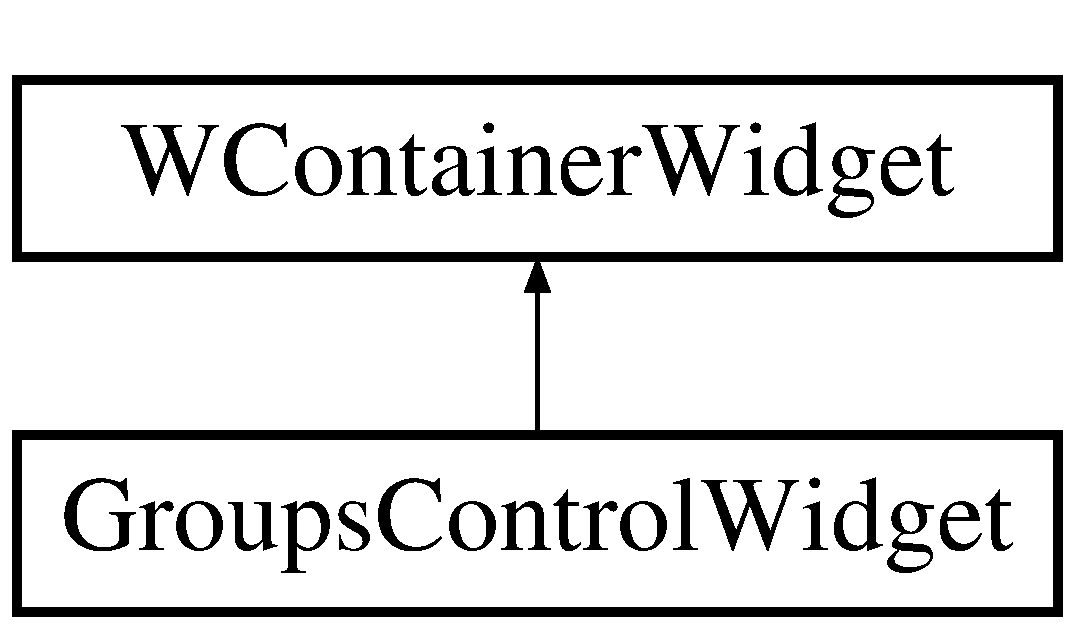
\includegraphics[height=2.000000cm]{class_groups_control_widget}
\end{center}
\end{figure}
\subsection*{Public Member Functions}
\begin{DoxyCompactItemize}
\item 
\hyperlink{class_groups_control_widget_a4d6a0e40f6968c53e163c167612932d4}{Groups\+Control\+Widget} (\hyperlink{class_session}{Session} $\ast$session, Wt\+::\+W\+Container\+Widget $\ast$parent=0)
\begin{DoxyCompactList}\small\item\em creates a \hyperlink{class_groups_control_widget}{Groups\+Control\+Widget} \end{DoxyCompactList}\item 
void \hyperlink{class_groups_control_widget_a6b7f7244d67dcdc7e1e946e0e1959f8d}{update} ()
\begin{DoxyCompactList}\small\item\em loads \hyperlink{class_single_groups_control_widget}{Single\+Groups\+Control\+Widget} page \end{DoxyCompactList}\end{DoxyCompactItemize}
\subsection*{Private Member Functions}
\begin{DoxyCompactItemize}
\item 
Wt\+::\+Http\+::\+Client $\ast$ \hyperlink{class_groups_control_widget_ac6dc70e7eccf6d30701c15d625424c0c}{connect} ()
\begin{DoxyCompactList}\small\item\em creates an H\+T\+TP Client \end{DoxyCompactList}\item 
void \hyperlink{class_groups_control_widget_a801b235a88f796198f1a65fcbe13c725}{light\+One} ()
\begin{DoxyCompactList}\small\item\em selects light 1 to be added to the group \end{DoxyCompactList}\item 
void \hyperlink{class_groups_control_widget_a28fa2a1848d1358587a37651861be081}{light\+Two} ()
\begin{DoxyCompactList}\small\item\em selects light 2 to be added to the group \end{DoxyCompactList}\item 
void \hyperlink{class_groups_control_widget_aaa514da760a67d4bf3e1ab7e51ea08f0}{light\+Three} ()
\begin{DoxyCompactList}\small\item\em selects light 3 to be added to the group \end{DoxyCompactList}\item 
void \hyperlink{class_groups_control_widget_a891bad4ba589f7bd7be8cb09a0910f20}{create\+Group} ()
\begin{DoxyCompactList}\small\item\em creates a new group \end{DoxyCompactList}\item 
void \hyperlink{class_groups_control_widget_a4fd7d26972133feb20b6941dc191535f}{return\+Bridge} ()
\begin{DoxyCompactList}\small\item\em returns user to bridge page \end{DoxyCompactList}\item 
void \hyperlink{class_groups_control_widget_ad5282b45d7e299bdac0813a8a72f6d3a}{handle\+Http\+Response} (boost\+::system\+::error\+\_\+code err, const Wt\+::\+Http\+::\+Message \&response)
\begin{DoxyCompactList}\small\item\em handles response and displays group information \end{DoxyCompactList}\item 
void \hyperlink{class_groups_control_widget_ade80d514e591c307c4cc6c0fbb758896}{handle\+Http\+Response\+V\+O\+ID} (boost\+::system\+::error\+\_\+code err, const Wt\+::\+Http\+::\+Message \&response)
\begin{DoxyCompactList}\small\item\em handles response and does nothing \end{DoxyCompactList}\end{DoxyCompactItemize}
\subsection*{Private Attributes}
\begin{DoxyCompactItemize}
\item 
\hyperlink{class_session}{Session} $\ast$ \hyperlink{class_groups_control_widget_a22dc704f954395ff53d67c51dbec933f}{session\+\_\+}
\item 
std\+::string \hyperlink{class_groups_control_widget_abf7a784bfb01b064e2bb2064c8e3e3a3}{ip} = \char`\"{}\char`\"{}
\item 
std\+::string \hyperlink{class_groups_control_widget_a5254fd01a7e3c5d56515d1161f392b09}{user\+ID} = \char`\"{}\char`\"{}
\item 
std\+::string \hyperlink{class_groups_control_widget_aad63d0d29a731819e47f1cd2974511ed}{port} = \char`\"{}\char`\"{}
\item 
bool \hyperlink{class_groups_control_widget_a83ab8b39f8c267cc46ad79b38e648618}{one} = false
\item 
bool \hyperlink{class_groups_control_widget_a4d0f1619ed1d0976fc48ea38262a5e5c}{two} = false
\item 
bool \hyperlink{class_groups_control_widget_a441299ffc41342f9c91d3d6f319732ed}{three} = false
\item 
Wt\+::\+W\+Line\+Edit $\ast$ \hyperlink{class_groups_control_widget_aecb5c19707326e3ec3c5b140da32e62d}{name\+Edit\+\_\+}
\item 
Wt\+::\+W\+Text $\ast$ \hyperlink{class_groups_control_widget_a66968632cf6001c9aeb5e227d9d06177}{light1\+\_\+}
\item 
Wt\+::\+W\+Text $\ast$ \hyperlink{class_groups_control_widget_aadce8705e32e8559e28feb2cfdae23e8}{light2\+\_\+}
\item 
Wt\+::\+W\+Text $\ast$ \hyperlink{class_groups_control_widget_a9846da1c58d8430074935daeea6b385b}{light3\+\_\+}
\item 
Wt\+::\+W\+Text $\ast$ \hyperlink{class_groups_control_widget_aa20f4ee341f245754611fa4494b38ecd}{status\+\_\+}
\end{DoxyCompactItemize}


\subsection{Constructor \& Destructor Documentation}
\mbox{\Hypertarget{class_groups_control_widget_a4d6a0e40f6968c53e163c167612932d4}\label{class_groups_control_widget_a4d6a0e40f6968c53e163c167612932d4}} 
\index{Groups\+Control\+Widget@{Groups\+Control\+Widget}!Groups\+Control\+Widget@{Groups\+Control\+Widget}}
\index{Groups\+Control\+Widget@{Groups\+Control\+Widget}!Groups\+Control\+Widget@{Groups\+Control\+Widget}}
\subsubsection{\texorpdfstring{Groups\+Control\+Widget()}{GroupsControlWidget()}}
{\footnotesize\ttfamily Groups\+Control\+Widget\+::\+Groups\+Control\+Widget (\begin{DoxyParamCaption}\item[{\hyperlink{class_session}{Session} $\ast$}]{session,  }\item[{Wt\+::\+W\+Container\+Widget $\ast$}]{parent = {\ttfamily 0} }\end{DoxyParamCaption})}



creates a \hyperlink{class_groups_control_widget}{Groups\+Control\+Widget} 


\begin{DoxyParams}{Parameters}
{\em session} & the database session \\
\hline
{\em parent} & the parent Widget Container \\
\hline
\end{DoxyParams}
\begin{DoxyReturn}{Returns}
\hyperlink{class_groups_control_widget}{Groups\+Control\+Widget} 
\end{DoxyReturn}


\subsection{Member Function Documentation}
\mbox{\Hypertarget{class_groups_control_widget_ac6dc70e7eccf6d30701c15d625424c0c}\label{class_groups_control_widget_ac6dc70e7eccf6d30701c15d625424c0c}} 
\index{Groups\+Control\+Widget@{Groups\+Control\+Widget}!connect@{connect}}
\index{connect@{connect}!Groups\+Control\+Widget@{Groups\+Control\+Widget}}
\subsubsection{\texorpdfstring{connect()}{connect()}}
{\footnotesize\ttfamily Http\+::\+Client $\ast$ Groups\+Control\+Widget\+::connect (\begin{DoxyParamCaption}{ }\end{DoxyParamCaption})\hspace{0.3cm}{\ttfamily [private]}}



creates an H\+T\+TP Client 

\begin{DoxyReturn}{Returns}
Http\+::\+Client 
\end{DoxyReturn}
\mbox{\Hypertarget{class_groups_control_widget_a891bad4ba589f7bd7be8cb09a0910f20}\label{class_groups_control_widget_a891bad4ba589f7bd7be8cb09a0910f20}} 
\index{Groups\+Control\+Widget@{Groups\+Control\+Widget}!create\+Group@{create\+Group}}
\index{create\+Group@{create\+Group}!Groups\+Control\+Widget@{Groups\+Control\+Widget}}
\subsubsection{\texorpdfstring{create\+Group()}{createGroup()}}
{\footnotesize\ttfamily void Groups\+Control\+Widget\+::create\+Group (\begin{DoxyParamCaption}{ }\end{DoxyParamCaption})\hspace{0.3cm}{\ttfamily [private]}}



creates a new group 

\begin{DoxyReturn}{Returns}
Void 
\end{DoxyReturn}
\mbox{\Hypertarget{class_groups_control_widget_ad5282b45d7e299bdac0813a8a72f6d3a}\label{class_groups_control_widget_ad5282b45d7e299bdac0813a8a72f6d3a}} 
\index{Groups\+Control\+Widget@{Groups\+Control\+Widget}!handle\+Http\+Response@{handle\+Http\+Response}}
\index{handle\+Http\+Response@{handle\+Http\+Response}!Groups\+Control\+Widget@{Groups\+Control\+Widget}}
\subsubsection{\texorpdfstring{handle\+Http\+Response()}{handleHttpResponse()}}
{\footnotesize\ttfamily void Groups\+Control\+Widget\+::handle\+Http\+Response (\begin{DoxyParamCaption}\item[{boost\+::system\+::error\+\_\+code}]{err,  }\item[{const Wt\+::\+Http\+::\+Message \&}]{response }\end{DoxyParamCaption})\hspace{0.3cm}{\ttfamily [private]}}



handles response and displays group information 


\begin{DoxyParams}{Parameters}
{\em err} & the response\textquotesingle{}s error code \\
\hline
{\em response} & the response \\
\hline
\end{DoxyParams}
\begin{DoxyReturn}{Returns}
Void 
\end{DoxyReturn}
\mbox{\Hypertarget{class_groups_control_widget_ade80d514e591c307c4cc6c0fbb758896}\label{class_groups_control_widget_ade80d514e591c307c4cc6c0fbb758896}} 
\index{Groups\+Control\+Widget@{Groups\+Control\+Widget}!handle\+Http\+Response\+V\+O\+ID@{handle\+Http\+Response\+V\+O\+ID}}
\index{handle\+Http\+Response\+V\+O\+ID@{handle\+Http\+Response\+V\+O\+ID}!Groups\+Control\+Widget@{Groups\+Control\+Widget}}
\subsubsection{\texorpdfstring{handle\+Http\+Response\+V\+O\+I\+D()}{handleHttpResponseVOID()}}
{\footnotesize\ttfamily void Groups\+Control\+Widget\+::handle\+Http\+Response\+V\+O\+ID (\begin{DoxyParamCaption}\item[{boost\+::system\+::error\+\_\+code}]{err,  }\item[{const Wt\+::\+Http\+::\+Message \&}]{response }\end{DoxyParamCaption})\hspace{0.3cm}{\ttfamily [private]}}



handles response and does nothing 


\begin{DoxyParams}{Parameters}
{\em err} & the response\textquotesingle{}s error code \\
\hline
{\em response} & the response \\
\hline
\end{DoxyParams}
\begin{DoxyReturn}{Returns}
Void 
\end{DoxyReturn}
\mbox{\Hypertarget{class_groups_control_widget_a801b235a88f796198f1a65fcbe13c725}\label{class_groups_control_widget_a801b235a88f796198f1a65fcbe13c725}} 
\index{Groups\+Control\+Widget@{Groups\+Control\+Widget}!light\+One@{light\+One}}
\index{light\+One@{light\+One}!Groups\+Control\+Widget@{Groups\+Control\+Widget}}
\subsubsection{\texorpdfstring{light\+One()}{lightOne()}}
{\footnotesize\ttfamily void Groups\+Control\+Widget\+::light\+One (\begin{DoxyParamCaption}{ }\end{DoxyParamCaption})\hspace{0.3cm}{\ttfamily [private]}}



selects light 1 to be added to the group 

\begin{DoxyReturn}{Returns}
Void 
\end{DoxyReturn}
\mbox{\Hypertarget{class_groups_control_widget_aaa514da760a67d4bf3e1ab7e51ea08f0}\label{class_groups_control_widget_aaa514da760a67d4bf3e1ab7e51ea08f0}} 
\index{Groups\+Control\+Widget@{Groups\+Control\+Widget}!light\+Three@{light\+Three}}
\index{light\+Three@{light\+Three}!Groups\+Control\+Widget@{Groups\+Control\+Widget}}
\subsubsection{\texorpdfstring{light\+Three()}{lightThree()}}
{\footnotesize\ttfamily void Groups\+Control\+Widget\+::light\+Three (\begin{DoxyParamCaption}{ }\end{DoxyParamCaption})\hspace{0.3cm}{\ttfamily [private]}}



selects light 3 to be added to the group 

\begin{DoxyReturn}{Returns}
Void 
\end{DoxyReturn}
\mbox{\Hypertarget{class_groups_control_widget_a28fa2a1848d1358587a37651861be081}\label{class_groups_control_widget_a28fa2a1848d1358587a37651861be081}} 
\index{Groups\+Control\+Widget@{Groups\+Control\+Widget}!light\+Two@{light\+Two}}
\index{light\+Two@{light\+Two}!Groups\+Control\+Widget@{Groups\+Control\+Widget}}
\subsubsection{\texorpdfstring{light\+Two()}{lightTwo()}}
{\footnotesize\ttfamily void Groups\+Control\+Widget\+::light\+Two (\begin{DoxyParamCaption}{ }\end{DoxyParamCaption})\hspace{0.3cm}{\ttfamily [private]}}



selects light 2 to be added to the group 

\begin{DoxyReturn}{Returns}
Void 
\end{DoxyReturn}
\mbox{\Hypertarget{class_groups_control_widget_a4fd7d26972133feb20b6941dc191535f}\label{class_groups_control_widget_a4fd7d26972133feb20b6941dc191535f}} 
\index{Groups\+Control\+Widget@{Groups\+Control\+Widget}!return\+Bridge@{return\+Bridge}}
\index{return\+Bridge@{return\+Bridge}!Groups\+Control\+Widget@{Groups\+Control\+Widget}}
\subsubsection{\texorpdfstring{return\+Bridge()}{returnBridge()}}
{\footnotesize\ttfamily void Groups\+Control\+Widget\+::return\+Bridge (\begin{DoxyParamCaption}{ }\end{DoxyParamCaption})\hspace{0.3cm}{\ttfamily [private]}}



returns user to bridge page 

\begin{DoxyReturn}{Returns}
Void 
\end{DoxyReturn}
\mbox{\Hypertarget{class_groups_control_widget_a6b7f7244d67dcdc7e1e946e0e1959f8d}\label{class_groups_control_widget_a6b7f7244d67dcdc7e1e946e0e1959f8d}} 
\index{Groups\+Control\+Widget@{Groups\+Control\+Widget}!update@{update}}
\index{update@{update}!Groups\+Control\+Widget@{Groups\+Control\+Widget}}
\subsubsection{\texorpdfstring{update()}{update()}}
{\footnotesize\ttfamily void Groups\+Control\+Widget\+::update (\begin{DoxyParamCaption}{ }\end{DoxyParamCaption})}



loads \hyperlink{class_single_groups_control_widget}{Single\+Groups\+Control\+Widget} page 

\begin{DoxyReturn}{Returns}
Void 
\end{DoxyReturn}


\subsection{Member Data Documentation}
\mbox{\Hypertarget{class_groups_control_widget_abf7a784bfb01b064e2bb2064c8e3e3a3}\label{class_groups_control_widget_abf7a784bfb01b064e2bb2064c8e3e3a3}} 
\index{Groups\+Control\+Widget@{Groups\+Control\+Widget}!ip@{ip}}
\index{ip@{ip}!Groups\+Control\+Widget@{Groups\+Control\+Widget}}
\subsubsection{\texorpdfstring{ip}{ip}}
{\footnotesize\ttfamily std\+::string Groups\+Control\+Widget\+::ip = \char`\"{}\char`\"{}\hspace{0.3cm}{\ttfamily [private]}}

bridge\textquotesingle{}s IP address \mbox{\Hypertarget{class_groups_control_widget_a66968632cf6001c9aeb5e227d9d06177}\label{class_groups_control_widget_a66968632cf6001c9aeb5e227d9d06177}} 
\index{Groups\+Control\+Widget@{Groups\+Control\+Widget}!light1\+\_\+@{light1\+\_\+}}
\index{light1\+\_\+@{light1\+\_\+}!Groups\+Control\+Widget@{Groups\+Control\+Widget}}
\subsubsection{\texorpdfstring{light1\+\_\+}{light1\_}}
{\footnotesize\ttfamily Wt\+::\+W\+Text$\ast$ Groups\+Control\+Widget\+::light1\+\_\+\hspace{0.3cm}{\ttfamily [private]}}

displays whether light 1 is part of the new group \mbox{\Hypertarget{class_groups_control_widget_aadce8705e32e8559e28feb2cfdae23e8}\label{class_groups_control_widget_aadce8705e32e8559e28feb2cfdae23e8}} 
\index{Groups\+Control\+Widget@{Groups\+Control\+Widget}!light2\+\_\+@{light2\+\_\+}}
\index{light2\+\_\+@{light2\+\_\+}!Groups\+Control\+Widget@{Groups\+Control\+Widget}}
\subsubsection{\texorpdfstring{light2\+\_\+}{light2\_}}
{\footnotesize\ttfamily Wt\+::\+W\+Text$\ast$ Groups\+Control\+Widget\+::light2\+\_\+\hspace{0.3cm}{\ttfamily [private]}}

displays whether light 2 is part of the new group \mbox{\Hypertarget{class_groups_control_widget_a9846da1c58d8430074935daeea6b385b}\label{class_groups_control_widget_a9846da1c58d8430074935daeea6b385b}} 
\index{Groups\+Control\+Widget@{Groups\+Control\+Widget}!light3\+\_\+@{light3\+\_\+}}
\index{light3\+\_\+@{light3\+\_\+}!Groups\+Control\+Widget@{Groups\+Control\+Widget}}
\subsubsection{\texorpdfstring{light3\+\_\+}{light3\_}}
{\footnotesize\ttfamily Wt\+::\+W\+Text$\ast$ Groups\+Control\+Widget\+::light3\+\_\+\hspace{0.3cm}{\ttfamily [private]}}

displays whether light 3 is part of the new group \mbox{\Hypertarget{class_groups_control_widget_aecb5c19707326e3ec3c5b140da32e62d}\label{class_groups_control_widget_aecb5c19707326e3ec3c5b140da32e62d}} 
\index{Groups\+Control\+Widget@{Groups\+Control\+Widget}!name\+Edit\+\_\+@{name\+Edit\+\_\+}}
\index{name\+Edit\+\_\+@{name\+Edit\+\_\+}!Groups\+Control\+Widget@{Groups\+Control\+Widget}}
\subsubsection{\texorpdfstring{name\+Edit\+\_\+}{nameEdit\_}}
{\footnotesize\ttfamily Wt\+::\+W\+Line\+Edit$\ast$ Groups\+Control\+Widget\+::name\+Edit\+\_\+\hspace{0.3cm}{\ttfamily [private]}}

new group\textquotesingle{}s name \mbox{\Hypertarget{class_groups_control_widget_a83ab8b39f8c267cc46ad79b38e648618}\label{class_groups_control_widget_a83ab8b39f8c267cc46ad79b38e648618}} 
\index{Groups\+Control\+Widget@{Groups\+Control\+Widget}!one@{one}}
\index{one@{one}!Groups\+Control\+Widget@{Groups\+Control\+Widget}}
\subsubsection{\texorpdfstring{one}{one}}
{\footnotesize\ttfamily bool Groups\+Control\+Widget\+::one = false\hspace{0.3cm}{\ttfamily [private]}}

status of light 1\textquotesingle{}s membership in the new group \mbox{\Hypertarget{class_groups_control_widget_aad63d0d29a731819e47f1cd2974511ed}\label{class_groups_control_widget_aad63d0d29a731819e47f1cd2974511ed}} 
\index{Groups\+Control\+Widget@{Groups\+Control\+Widget}!port@{port}}
\index{port@{port}!Groups\+Control\+Widget@{Groups\+Control\+Widget}}
\subsubsection{\texorpdfstring{port}{port}}
{\footnotesize\ttfamily std\+::string Groups\+Control\+Widget\+::port = \char`\"{}\char`\"{}\hspace{0.3cm}{\ttfamily [private]}}

bridge\textquotesingle{}s port number \mbox{\Hypertarget{class_groups_control_widget_a22dc704f954395ff53d67c51dbec933f}\label{class_groups_control_widget_a22dc704f954395ff53d67c51dbec933f}} 
\index{Groups\+Control\+Widget@{Groups\+Control\+Widget}!session\+\_\+@{session\+\_\+}}
\index{session\+\_\+@{session\+\_\+}!Groups\+Control\+Widget@{Groups\+Control\+Widget}}
\subsubsection{\texorpdfstring{session\+\_\+}{session\_}}
{\footnotesize\ttfamily \hyperlink{class_session}{Session}$\ast$ Groups\+Control\+Widget\+::session\+\_\+\hspace{0.3cm}{\ttfamily [private]}}

keeps track of group status \mbox{\Hypertarget{class_groups_control_widget_aa20f4ee341f245754611fa4494b38ecd}\label{class_groups_control_widget_aa20f4ee341f245754611fa4494b38ecd}} 
\index{Groups\+Control\+Widget@{Groups\+Control\+Widget}!status\+\_\+@{status\+\_\+}}
\index{status\+\_\+@{status\+\_\+}!Groups\+Control\+Widget@{Groups\+Control\+Widget}}
\subsubsection{\texorpdfstring{status\+\_\+}{status\_}}
{\footnotesize\ttfamily Wt\+::\+W\+Text$\ast$ Groups\+Control\+Widget\+::status\+\_\+\hspace{0.3cm}{\ttfamily [private]}}

status of creating a group \mbox{\Hypertarget{class_groups_control_widget_a441299ffc41342f9c91d3d6f319732ed}\label{class_groups_control_widget_a441299ffc41342f9c91d3d6f319732ed}} 
\index{Groups\+Control\+Widget@{Groups\+Control\+Widget}!three@{three}}
\index{three@{three}!Groups\+Control\+Widget@{Groups\+Control\+Widget}}
\subsubsection{\texorpdfstring{three}{three}}
{\footnotesize\ttfamily bool Groups\+Control\+Widget\+::three = false\hspace{0.3cm}{\ttfamily [private]}}

status of light 3\textquotesingle{}s membership in the new group \mbox{\Hypertarget{class_groups_control_widget_a4d0f1619ed1d0976fc48ea38262a5e5c}\label{class_groups_control_widget_a4d0f1619ed1d0976fc48ea38262a5e5c}} 
\index{Groups\+Control\+Widget@{Groups\+Control\+Widget}!two@{two}}
\index{two@{two}!Groups\+Control\+Widget@{Groups\+Control\+Widget}}
\subsubsection{\texorpdfstring{two}{two}}
{\footnotesize\ttfamily bool Groups\+Control\+Widget\+::two = false\hspace{0.3cm}{\ttfamily [private]}}

status of light 2\textquotesingle{}s membership in the new group \mbox{\Hypertarget{class_groups_control_widget_a5254fd01a7e3c5d56515d1161f392b09}\label{class_groups_control_widget_a5254fd01a7e3c5d56515d1161f392b09}} 
\index{Groups\+Control\+Widget@{Groups\+Control\+Widget}!user\+ID@{user\+ID}}
\index{user\+ID@{user\+ID}!Groups\+Control\+Widget@{Groups\+Control\+Widget}}
\subsubsection{\texorpdfstring{user\+ID}{userID}}
{\footnotesize\ttfamily std\+::string Groups\+Control\+Widget\+::user\+ID = \char`\"{}\char`\"{}\hspace{0.3cm}{\ttfamily [private]}}

user\textquotesingle{}s bridge ID 

The documentation for this class was generated from the following files\+:\begin{DoxyCompactItemize}
\item 
\hyperlink{_groups_control_8h}{Groups\+Control.\+h}\item 
\hyperlink{_groups_control_8_c}{Groups\+Control.\+C}\end{DoxyCompactItemize}

\hypertarget{class_hue_app}{}\section{Hue\+App Class Reference}
\label{class_hue_app}\index{Hue\+App@{Hue\+App}}


{\ttfamily \#include $<$Hue\+App.\+h$>$}

Inheritance diagram for Hue\+App\+:\begin{figure}[H]
\begin{center}
\leavevmode
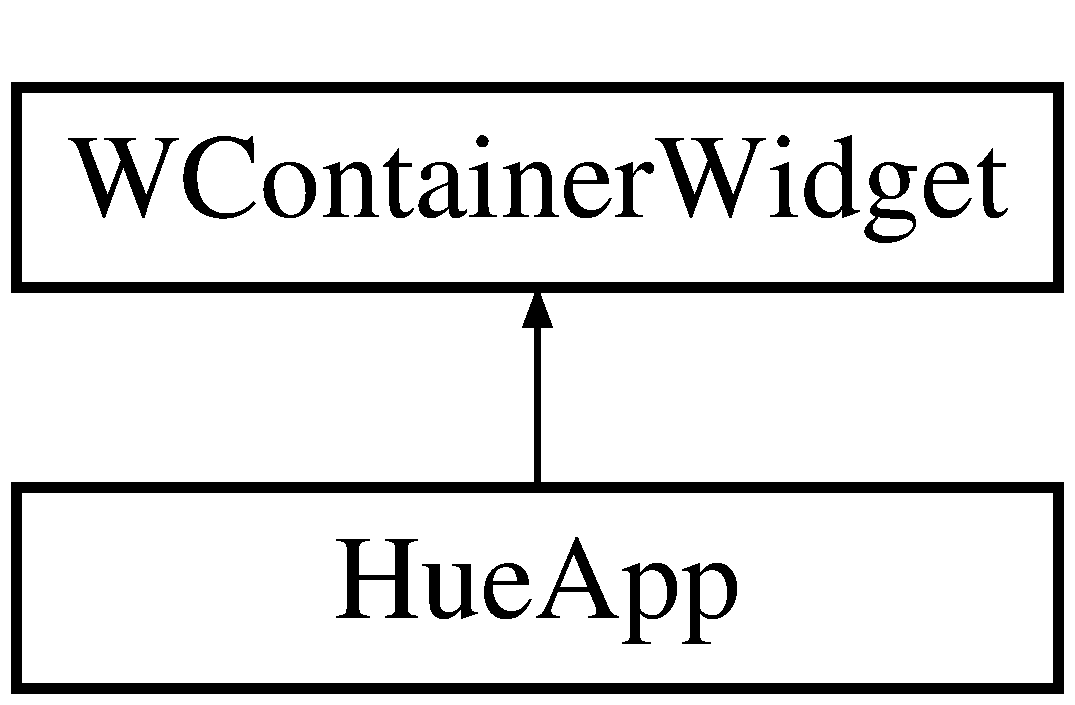
\includegraphics[height=2.000000cm]{class_hue_app}
\end{center}
\end{figure}
\subsection*{Public Member Functions}
\begin{DoxyCompactItemize}
\item 
\hyperlink{class_hue_app_a34bbbd56837e397473a85d9d6adc99fa}{Hue\+App} (Wt\+::\+W\+Container\+Widget $\ast$parent=0)
\item 
void \hyperlink{class_hue_app_a434baacf5c3e79b09cbedf8057060cbb}{handle\+Internal\+Path} (const std\+::string \&internal\+Path)
\end{DoxyCompactItemize}
\subsection*{Private Member Functions}
\begin{DoxyCompactItemize}
\item 
void \hyperlink{class_hue_app_af349923ea5d293c0226efd3ef71f4616}{on\+Auth\+Event} ()
\item 
void \hyperlink{class_hue_app_a3f5ea7541b2a416acd0b9f4e94073e72}{show\+Lights} ()
\item 
void \hyperlink{class_hue_app_a9e30cb9f84bfdc63261c6273cf07d5b1}{show\+Bridge} ()
\item 
void \hyperlink{class_hue_app_a05c48b318d651f27237ab6fc3c66c33b}{show\+Groups} ()
\item 
void \hyperlink{class_hue_app_a096902db63e23b1efb5756010af69209}{show\+Single\+Groups} ()
\item 
void \hyperlink{class_hue_app_a889374816e88dddf42d7dc44732dbc3a}{show\+Schedulers} ()
\end{DoxyCompactItemize}
\subsection*{Private Attributes}
\begin{DoxyCompactItemize}
\item 
Wt\+::\+W\+Stacked\+Widget $\ast$ \hyperlink{class_hue_app_a9ed5493a6b9a1651c8ad035c656d15e5}{main\+Stack\+\_\+}
\item 
\hyperlink{class_lights_control_widget}{Lights\+Control\+Widget} $\ast$ \hyperlink{class_hue_app_af56dcc0d22552d50417533c087816599}{the\+\_\+\+Lights}
\item 
\hyperlink{class_bridge_control_widget}{Bridge\+Control\+Widget} $\ast$ \hyperlink{class_hue_app_a6ec8432c5f76ef8c5799da130d39965c}{the\+\_\+\+Bridge}
\item 
\hyperlink{class_groups_control_widget}{Groups\+Control\+Widget} $\ast$ \hyperlink{class_hue_app_ae8a1698036628944f71e6bb985de7335}{the\+\_\+\+Groups}
\item 
\hyperlink{class_single_groups_control_widget}{Single\+Groups\+Control\+Widget} $\ast$ \hyperlink{class_hue_app_aa13e55cb1398a69aa97a8848d0981637}{the\+\_\+\+Single\+Groups}
\item 
\hyperlink{class_scheduler_control_widget}{Scheduler\+Control\+Widget} $\ast$ \hyperlink{class_hue_app_ae31f2868c0c0123f27ca4d60f7d63c0b}{the\+\_\+\+Schedulers}
\item 
Wt\+::\+W\+Anchor $\ast$ \hyperlink{class_hue_app_a76a68ad13aca8a4d13558ce355f02278}{back\+To\+Game\+Anchor\+\_\+}
\item 
\hyperlink{class_session}{Session} \hyperlink{class_hue_app_a38aedace7f2be9252275e24d8e09f46f}{session\+\_\+}
\end{DoxyCompactItemize}


\subsection{Constructor \& Destructor Documentation}
\mbox{\Hypertarget{class_hue_app_a34bbbd56837e397473a85d9d6adc99fa}\label{class_hue_app_a34bbbd56837e397473a85d9d6adc99fa}} 
\index{Hue\+App@{Hue\+App}!Hue\+App@{Hue\+App}}
\index{Hue\+App@{Hue\+App}!Hue\+App@{Hue\+App}}
\subsubsection{\texorpdfstring{Hue\+App()}{HueApp()}}
{\footnotesize\ttfamily Hue\+App\+::\+Hue\+App (\begin{DoxyParamCaption}\item[{Wt\+::\+W\+Container\+Widget $\ast$}]{parent = {\ttfamily 0} }\end{DoxyParamCaption})}



\subsection{Member Function Documentation}
\mbox{\Hypertarget{class_hue_app_a434baacf5c3e79b09cbedf8057060cbb}\label{class_hue_app_a434baacf5c3e79b09cbedf8057060cbb}} 
\index{Hue\+App@{Hue\+App}!handle\+Internal\+Path@{handle\+Internal\+Path}}
\index{handle\+Internal\+Path@{handle\+Internal\+Path}!Hue\+App@{Hue\+App}}
\subsubsection{\texorpdfstring{handle\+Internal\+Path()}{handleInternalPath()}}
{\footnotesize\ttfamily void Hue\+App\+::handle\+Internal\+Path (\begin{DoxyParamCaption}\item[{const std\+::string \&}]{internal\+Path }\end{DoxyParamCaption})}

\mbox{\Hypertarget{class_hue_app_af349923ea5d293c0226efd3ef71f4616}\label{class_hue_app_af349923ea5d293c0226efd3ef71f4616}} 
\index{Hue\+App@{Hue\+App}!on\+Auth\+Event@{on\+Auth\+Event}}
\index{on\+Auth\+Event@{on\+Auth\+Event}!Hue\+App@{Hue\+App}}
\subsubsection{\texorpdfstring{on\+Auth\+Event()}{onAuthEvent()}}
{\footnotesize\ttfamily void Hue\+App\+::on\+Auth\+Event (\begin{DoxyParamCaption}{ }\end{DoxyParamCaption})\hspace{0.3cm}{\ttfamily [private]}}

\mbox{\Hypertarget{class_hue_app_a9e30cb9f84bfdc63261c6273cf07d5b1}\label{class_hue_app_a9e30cb9f84bfdc63261c6273cf07d5b1}} 
\index{Hue\+App@{Hue\+App}!show\+Bridge@{show\+Bridge}}
\index{show\+Bridge@{show\+Bridge}!Hue\+App@{Hue\+App}}
\subsubsection{\texorpdfstring{show\+Bridge()}{showBridge()}}
{\footnotesize\ttfamily void Hue\+App\+::show\+Bridge (\begin{DoxyParamCaption}{ }\end{DoxyParamCaption})\hspace{0.3cm}{\ttfamily [private]}}

\mbox{\Hypertarget{class_hue_app_a05c48b318d651f27237ab6fc3c66c33b}\label{class_hue_app_a05c48b318d651f27237ab6fc3c66c33b}} 
\index{Hue\+App@{Hue\+App}!show\+Groups@{show\+Groups}}
\index{show\+Groups@{show\+Groups}!Hue\+App@{Hue\+App}}
\subsubsection{\texorpdfstring{show\+Groups()}{showGroups()}}
{\footnotesize\ttfamily void Hue\+App\+::show\+Groups (\begin{DoxyParamCaption}{ }\end{DoxyParamCaption})\hspace{0.3cm}{\ttfamily [private]}}

\mbox{\Hypertarget{class_hue_app_a3f5ea7541b2a416acd0b9f4e94073e72}\label{class_hue_app_a3f5ea7541b2a416acd0b9f4e94073e72}} 
\index{Hue\+App@{Hue\+App}!show\+Lights@{show\+Lights}}
\index{show\+Lights@{show\+Lights}!Hue\+App@{Hue\+App}}
\subsubsection{\texorpdfstring{show\+Lights()}{showLights()}}
{\footnotesize\ttfamily void Hue\+App\+::show\+Lights (\begin{DoxyParamCaption}{ }\end{DoxyParamCaption})\hspace{0.3cm}{\ttfamily [private]}}

\mbox{\Hypertarget{class_hue_app_a889374816e88dddf42d7dc44732dbc3a}\label{class_hue_app_a889374816e88dddf42d7dc44732dbc3a}} 
\index{Hue\+App@{Hue\+App}!show\+Schedulers@{show\+Schedulers}}
\index{show\+Schedulers@{show\+Schedulers}!Hue\+App@{Hue\+App}}
\subsubsection{\texorpdfstring{show\+Schedulers()}{showSchedulers()}}
{\footnotesize\ttfamily void Hue\+App\+::show\+Schedulers (\begin{DoxyParamCaption}{ }\end{DoxyParamCaption})\hspace{0.3cm}{\ttfamily [private]}}

\mbox{\Hypertarget{class_hue_app_a096902db63e23b1efb5756010af69209}\label{class_hue_app_a096902db63e23b1efb5756010af69209}} 
\index{Hue\+App@{Hue\+App}!show\+Single\+Groups@{show\+Single\+Groups}}
\index{show\+Single\+Groups@{show\+Single\+Groups}!Hue\+App@{Hue\+App}}
\subsubsection{\texorpdfstring{show\+Single\+Groups()}{showSingleGroups()}}
{\footnotesize\ttfamily void Hue\+App\+::show\+Single\+Groups (\begin{DoxyParamCaption}{ }\end{DoxyParamCaption})\hspace{0.3cm}{\ttfamily [private]}}



\subsection{Member Data Documentation}
\mbox{\Hypertarget{class_hue_app_a76a68ad13aca8a4d13558ce355f02278}\label{class_hue_app_a76a68ad13aca8a4d13558ce355f02278}} 
\index{Hue\+App@{Hue\+App}!back\+To\+Game\+Anchor\+\_\+@{back\+To\+Game\+Anchor\+\_\+}}
\index{back\+To\+Game\+Anchor\+\_\+@{back\+To\+Game\+Anchor\+\_\+}!Hue\+App@{Hue\+App}}
\subsubsection{\texorpdfstring{back\+To\+Game\+Anchor\+\_\+}{backToGameAnchor\_}}
{\footnotesize\ttfamily Wt\+::\+W\+Anchor$\ast$ Hue\+App\+::back\+To\+Game\+Anchor\+\_\+\hspace{0.3cm}{\ttfamily [private]}}

\mbox{\Hypertarget{class_hue_app_a9ed5493a6b9a1651c8ad035c656d15e5}\label{class_hue_app_a9ed5493a6b9a1651c8ad035c656d15e5}} 
\index{Hue\+App@{Hue\+App}!main\+Stack\+\_\+@{main\+Stack\+\_\+}}
\index{main\+Stack\+\_\+@{main\+Stack\+\_\+}!Hue\+App@{Hue\+App}}
\subsubsection{\texorpdfstring{main\+Stack\+\_\+}{mainStack\_}}
{\footnotesize\ttfamily Wt\+::\+W\+Stacked\+Widget$\ast$ Hue\+App\+::main\+Stack\+\_\+\hspace{0.3cm}{\ttfamily [private]}}

\mbox{\Hypertarget{class_hue_app_a38aedace7f2be9252275e24d8e09f46f}\label{class_hue_app_a38aedace7f2be9252275e24d8e09f46f}} 
\index{Hue\+App@{Hue\+App}!session\+\_\+@{session\+\_\+}}
\index{session\+\_\+@{session\+\_\+}!Hue\+App@{Hue\+App}}
\subsubsection{\texorpdfstring{session\+\_\+}{session\_}}
{\footnotesize\ttfamily \hyperlink{class_session}{Session} Hue\+App\+::session\+\_\+\hspace{0.3cm}{\ttfamily [private]}}

\mbox{\Hypertarget{class_hue_app_a6ec8432c5f76ef8c5799da130d39965c}\label{class_hue_app_a6ec8432c5f76ef8c5799da130d39965c}} 
\index{Hue\+App@{Hue\+App}!the\+\_\+\+Bridge@{the\+\_\+\+Bridge}}
\index{the\+\_\+\+Bridge@{the\+\_\+\+Bridge}!Hue\+App@{Hue\+App}}
\subsubsection{\texorpdfstring{the\+\_\+\+Bridge}{the\_Bridge}}
{\footnotesize\ttfamily \hyperlink{class_bridge_control_widget}{Bridge\+Control\+Widget}$\ast$ Hue\+App\+::the\+\_\+\+Bridge\hspace{0.3cm}{\ttfamily [private]}}

\mbox{\Hypertarget{class_hue_app_ae8a1698036628944f71e6bb985de7335}\label{class_hue_app_ae8a1698036628944f71e6bb985de7335}} 
\index{Hue\+App@{Hue\+App}!the\+\_\+\+Groups@{the\+\_\+\+Groups}}
\index{the\+\_\+\+Groups@{the\+\_\+\+Groups}!Hue\+App@{Hue\+App}}
\subsubsection{\texorpdfstring{the\+\_\+\+Groups}{the\_Groups}}
{\footnotesize\ttfamily \hyperlink{class_groups_control_widget}{Groups\+Control\+Widget}$\ast$ Hue\+App\+::the\+\_\+\+Groups\hspace{0.3cm}{\ttfamily [private]}}

\mbox{\Hypertarget{class_hue_app_af56dcc0d22552d50417533c087816599}\label{class_hue_app_af56dcc0d22552d50417533c087816599}} 
\index{Hue\+App@{Hue\+App}!the\+\_\+\+Lights@{the\+\_\+\+Lights}}
\index{the\+\_\+\+Lights@{the\+\_\+\+Lights}!Hue\+App@{Hue\+App}}
\subsubsection{\texorpdfstring{the\+\_\+\+Lights}{the\_Lights}}
{\footnotesize\ttfamily \hyperlink{class_lights_control_widget}{Lights\+Control\+Widget}$\ast$ Hue\+App\+::the\+\_\+\+Lights\hspace{0.3cm}{\ttfamily [private]}}

\mbox{\Hypertarget{class_hue_app_ae31f2868c0c0123f27ca4d60f7d63c0b}\label{class_hue_app_ae31f2868c0c0123f27ca4d60f7d63c0b}} 
\index{Hue\+App@{Hue\+App}!the\+\_\+\+Schedulers@{the\+\_\+\+Schedulers}}
\index{the\+\_\+\+Schedulers@{the\+\_\+\+Schedulers}!Hue\+App@{Hue\+App}}
\subsubsection{\texorpdfstring{the\+\_\+\+Schedulers}{the\_Schedulers}}
{\footnotesize\ttfamily \hyperlink{class_scheduler_control_widget}{Scheduler\+Control\+Widget}$\ast$ Hue\+App\+::the\+\_\+\+Schedulers\hspace{0.3cm}{\ttfamily [private]}}

\mbox{\Hypertarget{class_hue_app_aa13e55cb1398a69aa97a8848d0981637}\label{class_hue_app_aa13e55cb1398a69aa97a8848d0981637}} 
\index{Hue\+App@{Hue\+App}!the\+\_\+\+Single\+Groups@{the\+\_\+\+Single\+Groups}}
\index{the\+\_\+\+Single\+Groups@{the\+\_\+\+Single\+Groups}!Hue\+App@{Hue\+App}}
\subsubsection{\texorpdfstring{the\+\_\+\+Single\+Groups}{the\_SingleGroups}}
{\footnotesize\ttfamily \hyperlink{class_single_groups_control_widget}{Single\+Groups\+Control\+Widget}$\ast$ Hue\+App\+::the\+\_\+\+Single\+Groups\hspace{0.3cm}{\ttfamily [private]}}



The documentation for this class was generated from the following files\+:\begin{DoxyCompactItemize}
\item 
\hyperlink{_hue_app_8h}{Hue\+App.\+h}\item 
\hyperlink{_hue_app_8_c}{Hue\+App.\+C}\end{DoxyCompactItemize}

\hypertarget{class_light}{}\section{Light Class Reference}
\label{class_light}\index{Light@{Light}}


{\ttfamily \#include $<$Light.\+h$>$}

\subsection*{Public Member Functions}
\begin{DoxyCompactItemize}
\item 
\hyperlink{class_light_aaeb13d35d2c08e223ca32e8382e83452}{Light} (std\+::string n\+Name, std\+::string n\+Type, int n\+Bri, int n\+Hue, int n\+Sat, bool n\+On, int n\+Trans)
\item 
\hyperlink{class_light_aeb5df09a25a32f19fdffa761268ba24f}{Light} ()
\item 
\hyperlink{class_light_ad0e59fad13bb6cfadc25b2c477e9ddc7}{$\sim$\+Light} ()
\item 
std\+::string \hyperlink{class_light_a768a0219abfdc1684e90513995280b08}{get\+Name} (void)
\item 
std\+::string \hyperlink{class_light_a8dfd61470ed66935ef3ea2de76d7049a}{get\+Type} (void)
\item 
int \hyperlink{class_light_ad512a50c53993d50ef98731d7b1d6653}{get\+Brightness} (void)
\item 
int \hyperlink{class_light_abc39a64bfcc5b43088cefcd662956cb8}{get\+Hue} (void)
\item 
int \hyperlink{class_light_ab654f1c6ffbc3f79fc88d487449dd744}{get\+Saturation} (void)
\item 
bool \hyperlink{class_light_a4145a367202562504ccf4314f489d0eb}{get\+On} (void)
\item 
int \hyperlink{class_light_ab38069befb7f7ba10b8ee0cffaf89d57}{get\+Transition} (void)
\item 
void \hyperlink{class_light_acbb28a74fceea5fc98568b315e328eac}{set\+Name} (std\+::string new\+Name)
\item 
void \hyperlink{class_light_a9bc02e6694d481e938e2b9710fd3ff9f}{set\+Type} (std\+::string new\+Type)
\item 
void \hyperlink{class_light_a26ebe8e6574a11c2e2a50c00378a3cea}{set\+Brightness} (int new\+Bri)
\item 
void \hyperlink{class_light_a1120d4aff3fcb5a1df425f7d08224691}{set\+Hue} (int new\+Hue)
\item 
void \hyperlink{class_light_a81c65b7b6a3cb135a69591c0640cd5e9}{set\+Saturation} (int new\+Sat)
\item 
void \hyperlink{class_light_abebbcc06640fed324f219f97bbe9ebc8}{set\+On} (bool new\+On)
\item 
void \hyperlink{class_light_a2daccaa69755e4397a85a830c7caaba1}{set\+Transition} (int new\+Trans)
\item 
{\footnotesize template$<$class Action $>$ }\\void \hyperlink{class_light_a2c527298bf267abdca3b30d3ebbf785e}{persist} (Action \&a)
\end{DoxyCompactItemize}
\subsection*{Private Attributes}
\begin{DoxyCompactItemize}
\item 
std\+::string \hyperlink{class_light_aed2e518d1e739c50c31ae77a865f51ed}{name}
\item 
std\+::string \hyperlink{class_light_a2825ae88a1158e927a6d16bea9175e56}{type}
\item 
bool \hyperlink{class_light_a37ee0b241dbdaff4a13cc269de33a8bf}{on}
\item 
int \hyperlink{class_light_a34001347a7ae6d2b3e0b12cfedc9aadf}{bri}
\item 
int \hyperlink{class_light_ae488614d58a7f0dec6ed59b59c6c37e9}{hue}
\item 
int \hyperlink{class_light_afbfb00988ab1c1e0a07fa20941c6f2bf}{sat}
\item 
int \hyperlink{class_light_abd73358fde9001da39f147d878f9dab8}{transition\+Time}
\item 
Wt\+::\+Dbo\+::ptr$<$ \hyperlink{class_bridge}{Bridge} $>$ \hyperlink{class_light_ab1491281b58c62b7031fc668e9e5b506}{bridge}
\end{DoxyCompactItemize}


\subsection{Constructor \& Destructor Documentation}
\mbox{\Hypertarget{class_light_aaeb13d35d2c08e223ca32e8382e83452}\label{class_light_aaeb13d35d2c08e223ca32e8382e83452}} 
\index{Light@{Light}!Light@{Light}}
\index{Light@{Light}!Light@{Light}}
\subsubsection{\texorpdfstring{Light()}{Light()}\hspace{0.1cm}{\footnotesize\ttfamily [1/2]}}
{\footnotesize\ttfamily Light\+::\+Light (\begin{DoxyParamCaption}\item[{std\+::string}]{n\+Name,  }\item[{std\+::string}]{n\+Type,  }\item[{int}]{n\+Bri,  }\item[{int}]{n\+Hue,  }\item[{int}]{n\+Sat,  }\item[{bool}]{n\+On,  }\item[{int}]{n\+Trans }\end{DoxyParamCaption})\hspace{0.3cm}{\ttfamily [inline]}}

\mbox{\Hypertarget{class_light_aeb5df09a25a32f19fdffa761268ba24f}\label{class_light_aeb5df09a25a32f19fdffa761268ba24f}} 
\index{Light@{Light}!Light@{Light}}
\index{Light@{Light}!Light@{Light}}
\subsubsection{\texorpdfstring{Light()}{Light()}\hspace{0.1cm}{\footnotesize\ttfamily [2/2]}}
{\footnotesize\ttfamily Light\+::\+Light (\begin{DoxyParamCaption}{ }\end{DoxyParamCaption})\hspace{0.3cm}{\ttfamily [inline]}}

\mbox{\Hypertarget{class_light_ad0e59fad13bb6cfadc25b2c477e9ddc7}\label{class_light_ad0e59fad13bb6cfadc25b2c477e9ddc7}} 
\index{Light@{Light}!````~Light@{$\sim$\+Light}}
\index{````~Light@{$\sim$\+Light}!Light@{Light}}
\subsubsection{\texorpdfstring{$\sim$\+Light()}{~Light()}}
{\footnotesize\ttfamily Light\+::$\sim$\+Light (\begin{DoxyParamCaption}{ }\end{DoxyParamCaption})\hspace{0.3cm}{\ttfamily [inline]}}



\subsection{Member Function Documentation}
\mbox{\Hypertarget{class_light_ad512a50c53993d50ef98731d7b1d6653}\label{class_light_ad512a50c53993d50ef98731d7b1d6653}} 
\index{Light@{Light}!get\+Brightness@{get\+Brightness}}
\index{get\+Brightness@{get\+Brightness}!Light@{Light}}
\subsubsection{\texorpdfstring{get\+Brightness()}{getBrightness()}}
{\footnotesize\ttfamily int Light\+::get\+Brightness (\begin{DoxyParamCaption}\item[{void}]{ }\end{DoxyParamCaption})\hspace{0.3cm}{\ttfamily [inline]}}

\mbox{\Hypertarget{class_light_abc39a64bfcc5b43088cefcd662956cb8}\label{class_light_abc39a64bfcc5b43088cefcd662956cb8}} 
\index{Light@{Light}!get\+Hue@{get\+Hue}}
\index{get\+Hue@{get\+Hue}!Light@{Light}}
\subsubsection{\texorpdfstring{get\+Hue()}{getHue()}}
{\footnotesize\ttfamily int Light\+::get\+Hue (\begin{DoxyParamCaption}\item[{void}]{ }\end{DoxyParamCaption})\hspace{0.3cm}{\ttfamily [inline]}}

\mbox{\Hypertarget{class_light_a768a0219abfdc1684e90513995280b08}\label{class_light_a768a0219abfdc1684e90513995280b08}} 
\index{Light@{Light}!get\+Name@{get\+Name}}
\index{get\+Name@{get\+Name}!Light@{Light}}
\subsubsection{\texorpdfstring{get\+Name()}{getName()}}
{\footnotesize\ttfamily std\+::string Light\+::get\+Name (\begin{DoxyParamCaption}\item[{void}]{ }\end{DoxyParamCaption})\hspace{0.3cm}{\ttfamily [inline]}}

\mbox{\Hypertarget{class_light_a4145a367202562504ccf4314f489d0eb}\label{class_light_a4145a367202562504ccf4314f489d0eb}} 
\index{Light@{Light}!get\+On@{get\+On}}
\index{get\+On@{get\+On}!Light@{Light}}
\subsubsection{\texorpdfstring{get\+On()}{getOn()}}
{\footnotesize\ttfamily bool Light\+::get\+On (\begin{DoxyParamCaption}\item[{void}]{ }\end{DoxyParamCaption})\hspace{0.3cm}{\ttfamily [inline]}}

\mbox{\Hypertarget{class_light_ab654f1c6ffbc3f79fc88d487449dd744}\label{class_light_ab654f1c6ffbc3f79fc88d487449dd744}} 
\index{Light@{Light}!get\+Saturation@{get\+Saturation}}
\index{get\+Saturation@{get\+Saturation}!Light@{Light}}
\subsubsection{\texorpdfstring{get\+Saturation()}{getSaturation()}}
{\footnotesize\ttfamily int Light\+::get\+Saturation (\begin{DoxyParamCaption}\item[{void}]{ }\end{DoxyParamCaption})\hspace{0.3cm}{\ttfamily [inline]}}

\mbox{\Hypertarget{class_light_ab38069befb7f7ba10b8ee0cffaf89d57}\label{class_light_ab38069befb7f7ba10b8ee0cffaf89d57}} 
\index{Light@{Light}!get\+Transition@{get\+Transition}}
\index{get\+Transition@{get\+Transition}!Light@{Light}}
\subsubsection{\texorpdfstring{get\+Transition()}{getTransition()}}
{\footnotesize\ttfamily int Light\+::get\+Transition (\begin{DoxyParamCaption}\item[{void}]{ }\end{DoxyParamCaption})\hspace{0.3cm}{\ttfamily [inline]}}

\mbox{\Hypertarget{class_light_a8dfd61470ed66935ef3ea2de76d7049a}\label{class_light_a8dfd61470ed66935ef3ea2de76d7049a}} 
\index{Light@{Light}!get\+Type@{get\+Type}}
\index{get\+Type@{get\+Type}!Light@{Light}}
\subsubsection{\texorpdfstring{get\+Type()}{getType()}}
{\footnotesize\ttfamily std\+::string Light\+::get\+Type (\begin{DoxyParamCaption}\item[{void}]{ }\end{DoxyParamCaption})\hspace{0.3cm}{\ttfamily [inline]}}

\mbox{\Hypertarget{class_light_a2c527298bf267abdca3b30d3ebbf785e}\label{class_light_a2c527298bf267abdca3b30d3ebbf785e}} 
\index{Light@{Light}!persist@{persist}}
\index{persist@{persist}!Light@{Light}}
\subsubsection{\texorpdfstring{persist()}{persist()}}
{\footnotesize\ttfamily template$<$class Action $>$ \\
void Light\+::persist (\begin{DoxyParamCaption}\item[{Action \&}]{a }\end{DoxyParamCaption})\hspace{0.3cm}{\ttfamily [inline]}}

\mbox{\Hypertarget{class_light_a26ebe8e6574a11c2e2a50c00378a3cea}\label{class_light_a26ebe8e6574a11c2e2a50c00378a3cea}} 
\index{Light@{Light}!set\+Brightness@{set\+Brightness}}
\index{set\+Brightness@{set\+Brightness}!Light@{Light}}
\subsubsection{\texorpdfstring{set\+Brightness()}{setBrightness()}}
{\footnotesize\ttfamily void Light\+::set\+Brightness (\begin{DoxyParamCaption}\item[{int}]{new\+Bri }\end{DoxyParamCaption})\hspace{0.3cm}{\ttfamily [inline]}}

\mbox{\Hypertarget{class_light_a1120d4aff3fcb5a1df425f7d08224691}\label{class_light_a1120d4aff3fcb5a1df425f7d08224691}} 
\index{Light@{Light}!set\+Hue@{set\+Hue}}
\index{set\+Hue@{set\+Hue}!Light@{Light}}
\subsubsection{\texorpdfstring{set\+Hue()}{setHue()}}
{\footnotesize\ttfamily void Light\+::set\+Hue (\begin{DoxyParamCaption}\item[{int}]{new\+Hue }\end{DoxyParamCaption})\hspace{0.3cm}{\ttfamily [inline]}}

\mbox{\Hypertarget{class_light_acbb28a74fceea5fc98568b315e328eac}\label{class_light_acbb28a74fceea5fc98568b315e328eac}} 
\index{Light@{Light}!set\+Name@{set\+Name}}
\index{set\+Name@{set\+Name}!Light@{Light}}
\subsubsection{\texorpdfstring{set\+Name()}{setName()}}
{\footnotesize\ttfamily void Light\+::set\+Name (\begin{DoxyParamCaption}\item[{std\+::string}]{new\+Name }\end{DoxyParamCaption})\hspace{0.3cm}{\ttfamily [inline]}}

\mbox{\Hypertarget{class_light_abebbcc06640fed324f219f97bbe9ebc8}\label{class_light_abebbcc06640fed324f219f97bbe9ebc8}} 
\index{Light@{Light}!set\+On@{set\+On}}
\index{set\+On@{set\+On}!Light@{Light}}
\subsubsection{\texorpdfstring{set\+On()}{setOn()}}
{\footnotesize\ttfamily void Light\+::set\+On (\begin{DoxyParamCaption}\item[{bool}]{new\+On }\end{DoxyParamCaption})\hspace{0.3cm}{\ttfamily [inline]}}

\mbox{\Hypertarget{class_light_a81c65b7b6a3cb135a69591c0640cd5e9}\label{class_light_a81c65b7b6a3cb135a69591c0640cd5e9}} 
\index{Light@{Light}!set\+Saturation@{set\+Saturation}}
\index{set\+Saturation@{set\+Saturation}!Light@{Light}}
\subsubsection{\texorpdfstring{set\+Saturation()}{setSaturation()}}
{\footnotesize\ttfamily void Light\+::set\+Saturation (\begin{DoxyParamCaption}\item[{int}]{new\+Sat }\end{DoxyParamCaption})\hspace{0.3cm}{\ttfamily [inline]}}

\mbox{\Hypertarget{class_light_a2daccaa69755e4397a85a830c7caaba1}\label{class_light_a2daccaa69755e4397a85a830c7caaba1}} 
\index{Light@{Light}!set\+Transition@{set\+Transition}}
\index{set\+Transition@{set\+Transition}!Light@{Light}}
\subsubsection{\texorpdfstring{set\+Transition()}{setTransition()}}
{\footnotesize\ttfamily void Light\+::set\+Transition (\begin{DoxyParamCaption}\item[{int}]{new\+Trans }\end{DoxyParamCaption})\hspace{0.3cm}{\ttfamily [inline]}}

\mbox{\Hypertarget{class_light_a9bc02e6694d481e938e2b9710fd3ff9f}\label{class_light_a9bc02e6694d481e938e2b9710fd3ff9f}} 
\index{Light@{Light}!set\+Type@{set\+Type}}
\index{set\+Type@{set\+Type}!Light@{Light}}
\subsubsection{\texorpdfstring{set\+Type()}{setType()}}
{\footnotesize\ttfamily void Light\+::set\+Type (\begin{DoxyParamCaption}\item[{std\+::string}]{new\+Type }\end{DoxyParamCaption})\hspace{0.3cm}{\ttfamily [inline]}}



\subsection{Member Data Documentation}
\mbox{\Hypertarget{class_light_a34001347a7ae6d2b3e0b12cfedc9aadf}\label{class_light_a34001347a7ae6d2b3e0b12cfedc9aadf}} 
\index{Light@{Light}!bri@{bri}}
\index{bri@{bri}!Light@{Light}}
\subsubsection{\texorpdfstring{bri}{bri}}
{\footnotesize\ttfamily int Light\+::bri\hspace{0.3cm}{\ttfamily [private]}}

\mbox{\Hypertarget{class_light_ab1491281b58c62b7031fc668e9e5b506}\label{class_light_ab1491281b58c62b7031fc668e9e5b506}} 
\index{Light@{Light}!bridge@{bridge}}
\index{bridge@{bridge}!Light@{Light}}
\subsubsection{\texorpdfstring{bridge}{bridge}}
{\footnotesize\ttfamily Wt\+::\+Dbo\+::ptr$<$\hyperlink{class_bridge}{Bridge}$>$ Light\+::bridge\hspace{0.3cm}{\ttfamily [private]}}

\mbox{\Hypertarget{class_light_ae488614d58a7f0dec6ed59b59c6c37e9}\label{class_light_ae488614d58a7f0dec6ed59b59c6c37e9}} 
\index{Light@{Light}!hue@{hue}}
\index{hue@{hue}!Light@{Light}}
\subsubsection{\texorpdfstring{hue}{hue}}
{\footnotesize\ttfamily int Light\+::hue\hspace{0.3cm}{\ttfamily [private]}}

\mbox{\Hypertarget{class_light_aed2e518d1e739c50c31ae77a865f51ed}\label{class_light_aed2e518d1e739c50c31ae77a865f51ed}} 
\index{Light@{Light}!name@{name}}
\index{name@{name}!Light@{Light}}
\subsubsection{\texorpdfstring{name}{name}}
{\footnotesize\ttfamily std\+::string Light\+::name\hspace{0.3cm}{\ttfamily [private]}}

\mbox{\Hypertarget{class_light_a37ee0b241dbdaff4a13cc269de33a8bf}\label{class_light_a37ee0b241dbdaff4a13cc269de33a8bf}} 
\index{Light@{Light}!on@{on}}
\index{on@{on}!Light@{Light}}
\subsubsection{\texorpdfstring{on}{on}}
{\footnotesize\ttfamily bool Light\+::on\hspace{0.3cm}{\ttfamily [private]}}

\mbox{\Hypertarget{class_light_afbfb00988ab1c1e0a07fa20941c6f2bf}\label{class_light_afbfb00988ab1c1e0a07fa20941c6f2bf}} 
\index{Light@{Light}!sat@{sat}}
\index{sat@{sat}!Light@{Light}}
\subsubsection{\texorpdfstring{sat}{sat}}
{\footnotesize\ttfamily int Light\+::sat\hspace{0.3cm}{\ttfamily [private]}}

\mbox{\Hypertarget{class_light_abd73358fde9001da39f147d878f9dab8}\label{class_light_abd73358fde9001da39f147d878f9dab8}} 
\index{Light@{Light}!transition\+Time@{transition\+Time}}
\index{transition\+Time@{transition\+Time}!Light@{Light}}
\subsubsection{\texorpdfstring{transition\+Time}{transitionTime}}
{\footnotesize\ttfamily int Light\+::transition\+Time\hspace{0.3cm}{\ttfamily [private]}}

\mbox{\Hypertarget{class_light_a2825ae88a1158e927a6d16bea9175e56}\label{class_light_a2825ae88a1158e927a6d16bea9175e56}} 
\index{Light@{Light}!type@{type}}
\index{type@{type}!Light@{Light}}
\subsubsection{\texorpdfstring{type}{type}}
{\footnotesize\ttfamily std\+::string Light\+::type\hspace{0.3cm}{\ttfamily [private]}}



The documentation for this class was generated from the following file\+:\begin{DoxyCompactItemize}
\item 
\hyperlink{_light_8h}{Light.\+h}\end{DoxyCompactItemize}

\hypertarget{class_lights_control_widget}{}\section{Lights\+Control\+Widget Class Reference}
\label{class_lights_control_widget}\index{Lights\+Control\+Widget@{Lights\+Control\+Widget}}


{\ttfamily \#include $<$Lights\+Control.\+h$>$}

Inheritance diagram for Lights\+Control\+Widget\+:\begin{figure}[H]
\begin{center}
\leavevmode
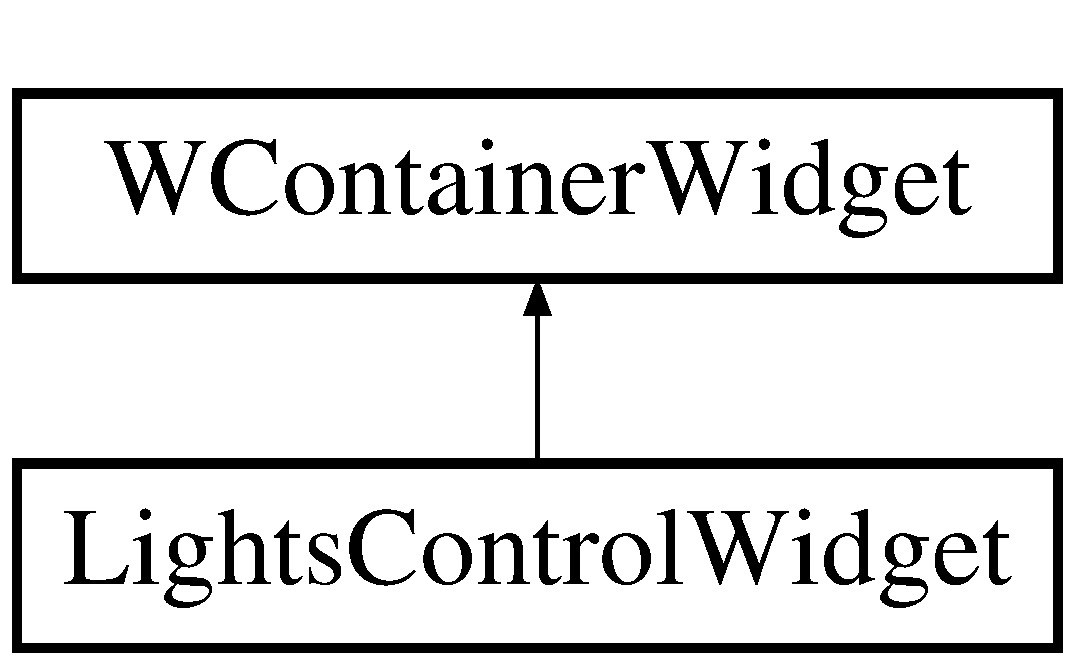
\includegraphics[height=2.000000cm]{class_lights_control_widget}
\end{center}
\end{figure}
\subsection*{Public Member Functions}
\begin{DoxyCompactItemize}
\item 
\hyperlink{class_lights_control_widget_a15e1439f70466b481134b8eba8f3cd5d}{Lights\+Control\+Widget} (\hyperlink{class_session}{Session} $\ast$session, Wt\+::\+W\+Container\+Widget $\ast$parent=0)
\begin{DoxyCompactList}\small\item\em creates a \hyperlink{class_lights_control_widget}{Lights\+Control\+Widget} \end{DoxyCompactList}\item 
void \hyperlink{class_lights_control_widget_a595489c5a7076eeaf32fee9d48bbd1fe}{update} ()
\begin{DoxyCompactList}\small\item\em loads \hyperlink{class_lights_control_widget}{Lights\+Control\+Widget} page \end{DoxyCompactList}\end{DoxyCompactItemize}
\subsection*{Private Member Functions}
\begin{DoxyCompactItemize}
\item 
Wt\+::\+Http\+::\+Client $\ast$ \hyperlink{class_lights_control_widget_a4a43f535b11a174e2f9a5b9ffe773557}{connect} ()
\begin{DoxyCompactList}\small\item\em creates an H\+T\+TP client \end{DoxyCompactList}\item 
void \hyperlink{class_lights_control_widget_ad5e2249e08c869e8bd9b190937b93f3c}{on} ()
\begin{DoxyCompactList}\small\item\em turns a light on \end{DoxyCompactList}\item 
void \hyperlink{class_lights_control_widget_a5d39b8ccaa59c8a8f0c8669b45cf0eb2}{off} ()
\begin{DoxyCompactList}\small\item\em turns a light off \end{DoxyCompactList}\item 
void \hyperlink{class_lights_control_widget_a9d7e8c4b0f0549a9a7c3ef96c4d5eef0}{hue} ()
\begin{DoxyCompactList}\small\item\em changes a light\textquotesingle{}s hue \end{DoxyCompactList}\item 
void \hyperlink{class_lights_control_widget_a05224e6a3f891fb29bbf85548aad4684}{bright} ()
\begin{DoxyCompactList}\small\item\em changes a light\textquotesingle{}s brightness \end{DoxyCompactList}\item 
void \hyperlink{class_lights_control_widget_a154f0a2b37fbbd67c920b392086ec60c}{sat} ()
\begin{DoxyCompactList}\small\item\em changes a light\textquotesingle{}s saturation \end{DoxyCompactList}\item 
void \hyperlink{class_lights_control_widget_aa0b663545779e7dd38fa61e456b158ec}{name} ()
\begin{DoxyCompactList}\small\item\em changes a light\textquotesingle{}s name \end{DoxyCompactList}\item 
void \hyperlink{class_lights_control_widget_a10fad17f0722f34402a906c77c1711bb}{transition} ()
\begin{DoxyCompactList}\small\item\em changes a light\textquotesingle{}s transition time \end{DoxyCompactList}\item 
void \hyperlink{class_lights_control_widget_aedb19ca01377b31ba326bd0e0f82138d}{light\+One} ()
\begin{DoxyCompactList}\small\item\em selects light 1 to change \end{DoxyCompactList}\item 
void \hyperlink{class_lights_control_widget_a8606dd33428f5c5cd7a1e686053b296d}{light\+Two} ()
\begin{DoxyCompactList}\small\item\em selects light 2 to change \end{DoxyCompactList}\item 
void \hyperlink{class_lights_control_widget_a670eae4637f1cc78febb3a751e4272dc}{light\+Three} ()
\begin{DoxyCompactList}\small\item\em selects light 3 to change \end{DoxyCompactList}\item 
void \hyperlink{class_lights_control_widget_a4b17ac832e826eb5665a8f69fe73c5f4}{return\+Bridge} ()
\begin{DoxyCompactList}\small\item\em returns user to the bridge page \end{DoxyCompactList}\item 
void \hyperlink{class_lights_control_widget_a0fd696e3500ca64cfeddd08738e5b6cf}{handle\+Http\+Response} (boost\+::system\+::error\+\_\+code err, const Wt\+::\+Http\+::\+Message \&response)
\begin{DoxyCompactList}\small\item\em handles response and displays light information \end{DoxyCompactList}\item 
void \hyperlink{class_lights_control_widget_ace0f0ce6387f25f695ac83a46a765a74}{handle\+Http\+Response\+Name} (boost\+::system\+::error\+\_\+code err, const Wt\+::\+Http\+::\+Message \&response)
\begin{DoxyCompactList}\small\item\em handles response for light name changes \end{DoxyCompactList}\item 
void \hyperlink{class_lights_control_widget_a9cc86543ee2df1d0bb09c35b0e2fac90}{handle\+Http\+Response\+V\+O\+ID} (boost\+::system\+::error\+\_\+code err, const Wt\+::\+Http\+::\+Message \&response)
\begin{DoxyCompactList}\small\item\em handles response and does nothing \end{DoxyCompactList}\end{DoxyCompactItemize}
\subsection*{Private Attributes}
\begin{DoxyCompactItemize}
\item 
\hyperlink{class_session}{Session} $\ast$session\+\_\+ std\+::string \hyperlink{class_lights_control_widget_a16eddbe64dce6b5fda5f52f5c35f41c0}{current\+Light} = \char`\"{}0\char`\"{}
\item 
std\+::string \hyperlink{class_lights_control_widget_aa2855e24d3d1afbcf6fcd2992abc47af}{ip} = \char`\"{}\char`\"{}
\item 
std\+::string \hyperlink{class_lights_control_widget_aa26d4553e677dec57b64575a6d6d8558}{user\+ID} = \char`\"{}\char`\"{}
\item 
std\+::string \hyperlink{class_lights_control_widget_a5760f7ec7c3c36e8faf00ae6b2633ab5}{port} = \char`\"{}\char`\"{}
\item 
Wt\+::\+W\+Line\+Edit $\ast$ \hyperlink{class_lights_control_widget_aff7b495c562df75a6006ad6bef43f96f}{name\+Edit\+\_\+}
\item 
Wt\+::\+W\+Slider $\ast$ \hyperlink{class_lights_control_widget_af957447fbfc39f4f0c87081be5cf2bf5}{sat\+Scale\+Slider\+\_\+}
\item 
Wt\+::\+W\+Slider $\ast$ \hyperlink{class_lights_control_widget_aafc30b2cc242d6ac2575128a491298d3}{bri\+Scale\+Slider\+\_\+}
\item 
Wt\+::\+W\+Slider $\ast$ \hyperlink{class_lights_control_widget_a71c03598de2481409316e7d1ca51fda0}{hue\+Scale\+Slider\+\_\+}
\item 
Wt\+::\+W\+Slider $\ast$ \hyperlink{class_lights_control_widget_af4bd66ddc5244ab9cf62dea9e5ffb1cf}{transition\+Scale\+Slider\+\_\+}
\item 
Wt\+::\+W\+Text $\ast$ \hyperlink{class_lights_control_widget_a5d33dac9a47a7862e6cc060e1e0fb335}{one\+Light\+\_\+}
\item 
Wt\+::\+W\+Text $\ast$two\+Light\+\_\+ Wt\+::\+W\+Text $\ast$ \hyperlink{class_lights_control_widget_adc837ede17eaef54ccd4b0a7e8749ebc}{three\+Light\+\_\+}
\item 
Wt\+::\+W\+Text $\ast$ \hyperlink{class_lights_control_widget_a27b0c91e6a4776c8b03dfc5324e3e365}{change\+\_\+}
\item 
Wt\+::\+W\+Text $\ast$ \hyperlink{class_lights_control_widget_a071eae068aef8f47a36e728ae3ad6378}{light\+\_\+}
\end{DoxyCompactItemize}


\subsection{Constructor \& Destructor Documentation}
\mbox{\Hypertarget{class_lights_control_widget_a15e1439f70466b481134b8eba8f3cd5d}\label{class_lights_control_widget_a15e1439f70466b481134b8eba8f3cd5d}} 
\index{Lights\+Control\+Widget@{Lights\+Control\+Widget}!Lights\+Control\+Widget@{Lights\+Control\+Widget}}
\index{Lights\+Control\+Widget@{Lights\+Control\+Widget}!Lights\+Control\+Widget@{Lights\+Control\+Widget}}
\subsubsection{\texorpdfstring{Lights\+Control\+Widget()}{LightsControlWidget()}}
{\footnotesize\ttfamily Lights\+Control\+Widget\+::\+Lights\+Control\+Widget (\begin{DoxyParamCaption}\item[{\hyperlink{class_session}{Session} $\ast$}]{session,  }\item[{Wt\+::\+W\+Container\+Widget $\ast$}]{parent = {\ttfamily 0} }\end{DoxyParamCaption})}



creates a \hyperlink{class_lights_control_widget}{Lights\+Control\+Widget} 


\begin{DoxyParams}{Parameters}
{\em session} & the database session \\
\hline
{\em parent} & the parent Widget Container \\
\hline
\end{DoxyParams}
\begin{DoxyReturn}{Returns}
\hyperlink{class_lights_control_widget}{Lights\+Control\+Widget} 
\end{DoxyReturn}

\begin{DoxyParams}{Parameters}
{\em session} & database session \\
\hline
{\em parent} & parent Widget Container \\
\hline
\end{DoxyParams}


\subsection{Member Function Documentation}
\mbox{\Hypertarget{class_lights_control_widget_a05224e6a3f891fb29bbf85548aad4684}\label{class_lights_control_widget_a05224e6a3f891fb29bbf85548aad4684}} 
\index{Lights\+Control\+Widget@{Lights\+Control\+Widget}!bright@{bright}}
\index{bright@{bright}!Lights\+Control\+Widget@{Lights\+Control\+Widget}}
\subsubsection{\texorpdfstring{bright()}{bright()}}
{\footnotesize\ttfamily void Lights\+Control\+Widget\+::bright (\begin{DoxyParamCaption}{ }\end{DoxyParamCaption})\hspace{0.3cm}{\ttfamily [private]}}



changes a light\textquotesingle{}s brightness 

\begin{DoxyReturn}{Returns}
Void 
\end{DoxyReturn}
\mbox{\Hypertarget{class_lights_control_widget_a4a43f535b11a174e2f9a5b9ffe773557}\label{class_lights_control_widget_a4a43f535b11a174e2f9a5b9ffe773557}} 
\index{Lights\+Control\+Widget@{Lights\+Control\+Widget}!connect@{connect}}
\index{connect@{connect}!Lights\+Control\+Widget@{Lights\+Control\+Widget}}
\subsubsection{\texorpdfstring{connect()}{connect()}}
{\footnotesize\ttfamily Http\+::\+Client $\ast$ Lights\+Control\+Widget\+::connect (\begin{DoxyParamCaption}{ }\end{DoxyParamCaption})\hspace{0.3cm}{\ttfamily [private]}}



creates an H\+T\+TP client 

\begin{DoxyReturn}{Returns}
Http\+::\+Client 
\end{DoxyReturn}
\mbox{\Hypertarget{class_lights_control_widget_a0fd696e3500ca64cfeddd08738e5b6cf}\label{class_lights_control_widget_a0fd696e3500ca64cfeddd08738e5b6cf}} 
\index{Lights\+Control\+Widget@{Lights\+Control\+Widget}!handle\+Http\+Response@{handle\+Http\+Response}}
\index{handle\+Http\+Response@{handle\+Http\+Response}!Lights\+Control\+Widget@{Lights\+Control\+Widget}}
\subsubsection{\texorpdfstring{handle\+Http\+Response()}{handleHttpResponse()}}
{\footnotesize\ttfamily void Lights\+Control\+Widget\+::handle\+Http\+Response (\begin{DoxyParamCaption}\item[{boost\+::system\+::error\+\_\+code}]{err,  }\item[{const Wt\+::\+Http\+::\+Message \&}]{response }\end{DoxyParamCaption})\hspace{0.3cm}{\ttfamily [private]}}



handles response and displays light information 


\begin{DoxyParams}{Parameters}
{\em err} & the response\textquotesingle{}s error code \\
\hline
{\em response} & the response \\
\hline
\end{DoxyParams}
\begin{DoxyReturn}{Returns}
Void 
\end{DoxyReturn}

\begin{DoxyParams}{Parameters}
{\em err} & error code \\
\hline
{\em response} & response \\
\hline
\end{DoxyParams}
\mbox{\Hypertarget{class_lights_control_widget_ace0f0ce6387f25f695ac83a46a765a74}\label{class_lights_control_widget_ace0f0ce6387f25f695ac83a46a765a74}} 
\index{Lights\+Control\+Widget@{Lights\+Control\+Widget}!handle\+Http\+Response\+Name@{handle\+Http\+Response\+Name}}
\index{handle\+Http\+Response\+Name@{handle\+Http\+Response\+Name}!Lights\+Control\+Widget@{Lights\+Control\+Widget}}
\subsubsection{\texorpdfstring{handle\+Http\+Response\+Name()}{handleHttpResponseName()}}
{\footnotesize\ttfamily void Lights\+Control\+Widget\+::handle\+Http\+Response\+Name (\begin{DoxyParamCaption}\item[{boost\+::system\+::error\+\_\+code}]{err,  }\item[{const Wt\+::\+Http\+::\+Message \&}]{response }\end{DoxyParamCaption})\hspace{0.3cm}{\ttfamily [private]}}



handles response for light name changes 


\begin{DoxyParams}{Parameters}
{\em err} & the response\textquotesingle{}s error code \\
\hline
{\em response} & the response \\
\hline
\end{DoxyParams}
\begin{DoxyReturn}{Returns}
Void 
\end{DoxyReturn}

\begin{DoxyParams}{Parameters}
{\em err} & error code \\
\hline
{\em response} & response \\
\hline
\end{DoxyParams}
\mbox{\Hypertarget{class_lights_control_widget_a9cc86543ee2df1d0bb09c35b0e2fac90}\label{class_lights_control_widget_a9cc86543ee2df1d0bb09c35b0e2fac90}} 
\index{Lights\+Control\+Widget@{Lights\+Control\+Widget}!handle\+Http\+Response\+V\+O\+ID@{handle\+Http\+Response\+V\+O\+ID}}
\index{handle\+Http\+Response\+V\+O\+ID@{handle\+Http\+Response\+V\+O\+ID}!Lights\+Control\+Widget@{Lights\+Control\+Widget}}
\subsubsection{\texorpdfstring{handle\+Http\+Response\+V\+O\+I\+D()}{handleHttpResponseVOID()}}
{\footnotesize\ttfamily void Lights\+Control\+Widget\+::handle\+Http\+Response\+V\+O\+ID (\begin{DoxyParamCaption}\item[{boost\+::system\+::error\+\_\+code}]{err,  }\item[{const Wt\+::\+Http\+::\+Message \&}]{response }\end{DoxyParamCaption})\hspace{0.3cm}{\ttfamily [private]}}



handles response and does nothing 


\begin{DoxyParams}{Parameters}
{\em err} & the response\textquotesingle{}s error code \\
\hline
{\em response} & the response \\
\hline
\end{DoxyParams}
\begin{DoxyReturn}{Returns}
Void 
\end{DoxyReturn}

\begin{DoxyParams}{Parameters}
{\em err} & error code \\
\hline
{\em response} & response \\
\hline
\end{DoxyParams}
\mbox{\Hypertarget{class_lights_control_widget_a9d7e8c4b0f0549a9a7c3ef96c4d5eef0}\label{class_lights_control_widget_a9d7e8c4b0f0549a9a7c3ef96c4d5eef0}} 
\index{Lights\+Control\+Widget@{Lights\+Control\+Widget}!hue@{hue}}
\index{hue@{hue}!Lights\+Control\+Widget@{Lights\+Control\+Widget}}
\subsubsection{\texorpdfstring{hue()}{hue()}}
{\footnotesize\ttfamily void Lights\+Control\+Widget\+::hue (\begin{DoxyParamCaption}{ }\end{DoxyParamCaption})\hspace{0.3cm}{\ttfamily [private]}}



changes a light\textquotesingle{}s hue 

\begin{DoxyReturn}{Returns}
Void 
\end{DoxyReturn}
\mbox{\Hypertarget{class_lights_control_widget_aedb19ca01377b31ba326bd0e0f82138d}\label{class_lights_control_widget_aedb19ca01377b31ba326bd0e0f82138d}} 
\index{Lights\+Control\+Widget@{Lights\+Control\+Widget}!light\+One@{light\+One}}
\index{light\+One@{light\+One}!Lights\+Control\+Widget@{Lights\+Control\+Widget}}
\subsubsection{\texorpdfstring{light\+One()}{lightOne()}}
{\footnotesize\ttfamily void Lights\+Control\+Widget\+::light\+One (\begin{DoxyParamCaption}{ }\end{DoxyParamCaption})\hspace{0.3cm}{\ttfamily [private]}}



selects light 1 to change 

\begin{DoxyReturn}{Returns}
Void 
\end{DoxyReturn}
\mbox{\Hypertarget{class_lights_control_widget_a670eae4637f1cc78febb3a751e4272dc}\label{class_lights_control_widget_a670eae4637f1cc78febb3a751e4272dc}} 
\index{Lights\+Control\+Widget@{Lights\+Control\+Widget}!light\+Three@{light\+Three}}
\index{light\+Three@{light\+Three}!Lights\+Control\+Widget@{Lights\+Control\+Widget}}
\subsubsection{\texorpdfstring{light\+Three()}{lightThree()}}
{\footnotesize\ttfamily void Lights\+Control\+Widget\+::light\+Three (\begin{DoxyParamCaption}{ }\end{DoxyParamCaption})\hspace{0.3cm}{\ttfamily [private]}}



selects light 3 to change 

\begin{DoxyReturn}{Returns}
Void 
\end{DoxyReturn}
\mbox{\Hypertarget{class_lights_control_widget_a8606dd33428f5c5cd7a1e686053b296d}\label{class_lights_control_widget_a8606dd33428f5c5cd7a1e686053b296d}} 
\index{Lights\+Control\+Widget@{Lights\+Control\+Widget}!light\+Two@{light\+Two}}
\index{light\+Two@{light\+Two}!Lights\+Control\+Widget@{Lights\+Control\+Widget}}
\subsubsection{\texorpdfstring{light\+Two()}{lightTwo()}}
{\footnotesize\ttfamily void Lights\+Control\+Widget\+::light\+Two (\begin{DoxyParamCaption}{ }\end{DoxyParamCaption})\hspace{0.3cm}{\ttfamily [private]}}



selects light 2 to change 

\begin{DoxyReturn}{Returns}
Void 
\end{DoxyReturn}
\mbox{\Hypertarget{class_lights_control_widget_aa0b663545779e7dd38fa61e456b158ec}\label{class_lights_control_widget_aa0b663545779e7dd38fa61e456b158ec}} 
\index{Lights\+Control\+Widget@{Lights\+Control\+Widget}!name@{name}}
\index{name@{name}!Lights\+Control\+Widget@{Lights\+Control\+Widget}}
\subsubsection{\texorpdfstring{name()}{name()}}
{\footnotesize\ttfamily void Lights\+Control\+Widget\+::name (\begin{DoxyParamCaption}{ }\end{DoxyParamCaption})\hspace{0.3cm}{\ttfamily [private]}}



changes a light\textquotesingle{}s name 

\begin{DoxyReturn}{Returns}
Void 
\end{DoxyReturn}
\mbox{\Hypertarget{class_lights_control_widget_a5d39b8ccaa59c8a8f0c8669b45cf0eb2}\label{class_lights_control_widget_a5d39b8ccaa59c8a8f0c8669b45cf0eb2}} 
\index{Lights\+Control\+Widget@{Lights\+Control\+Widget}!off@{off}}
\index{off@{off}!Lights\+Control\+Widget@{Lights\+Control\+Widget}}
\subsubsection{\texorpdfstring{off()}{off()}}
{\footnotesize\ttfamily void Lights\+Control\+Widget\+::off (\begin{DoxyParamCaption}{ }\end{DoxyParamCaption})\hspace{0.3cm}{\ttfamily [private]}}



turns a light off 

\begin{DoxyReturn}{Returns}
Void 
\end{DoxyReturn}
\mbox{\Hypertarget{class_lights_control_widget_ad5e2249e08c869e8bd9b190937b93f3c}\label{class_lights_control_widget_ad5e2249e08c869e8bd9b190937b93f3c}} 
\index{Lights\+Control\+Widget@{Lights\+Control\+Widget}!on@{on}}
\index{on@{on}!Lights\+Control\+Widget@{Lights\+Control\+Widget}}
\subsubsection{\texorpdfstring{on()}{on()}}
{\footnotesize\ttfamily void Lights\+Control\+Widget\+::on (\begin{DoxyParamCaption}{ }\end{DoxyParamCaption})\hspace{0.3cm}{\ttfamily [private]}}



turns a light on 

\begin{DoxyReturn}{Returns}
Void 
\end{DoxyReturn}
\mbox{\Hypertarget{class_lights_control_widget_a4b17ac832e826eb5665a8f69fe73c5f4}\label{class_lights_control_widget_a4b17ac832e826eb5665a8f69fe73c5f4}} 
\index{Lights\+Control\+Widget@{Lights\+Control\+Widget}!return\+Bridge@{return\+Bridge}}
\index{return\+Bridge@{return\+Bridge}!Lights\+Control\+Widget@{Lights\+Control\+Widget}}
\subsubsection{\texorpdfstring{return\+Bridge()}{returnBridge()}}
{\footnotesize\ttfamily void Lights\+Control\+Widget\+::return\+Bridge (\begin{DoxyParamCaption}{ }\end{DoxyParamCaption})\hspace{0.3cm}{\ttfamily [private]}}



returns user to the bridge page 

\begin{DoxyReturn}{Returns}
Void 
\end{DoxyReturn}
\mbox{\Hypertarget{class_lights_control_widget_a154f0a2b37fbbd67c920b392086ec60c}\label{class_lights_control_widget_a154f0a2b37fbbd67c920b392086ec60c}} 
\index{Lights\+Control\+Widget@{Lights\+Control\+Widget}!sat@{sat}}
\index{sat@{sat}!Lights\+Control\+Widget@{Lights\+Control\+Widget}}
\subsubsection{\texorpdfstring{sat()}{sat()}}
{\footnotesize\ttfamily void Lights\+Control\+Widget\+::sat (\begin{DoxyParamCaption}{ }\end{DoxyParamCaption})\hspace{0.3cm}{\ttfamily [private]}}



changes a light\textquotesingle{}s saturation 

\begin{DoxyReturn}{Returns}
Void 
\end{DoxyReturn}
\mbox{\Hypertarget{class_lights_control_widget_a10fad17f0722f34402a906c77c1711bb}\label{class_lights_control_widget_a10fad17f0722f34402a906c77c1711bb}} 
\index{Lights\+Control\+Widget@{Lights\+Control\+Widget}!transition@{transition}}
\index{transition@{transition}!Lights\+Control\+Widget@{Lights\+Control\+Widget}}
\subsubsection{\texorpdfstring{transition()}{transition()}}
{\footnotesize\ttfamily void Lights\+Control\+Widget\+::transition (\begin{DoxyParamCaption}{ }\end{DoxyParamCaption})\hspace{0.3cm}{\ttfamily [private]}}



changes a light\textquotesingle{}s transition time 

\begin{DoxyReturn}{Returns}
Void 
\end{DoxyReturn}
\mbox{\Hypertarget{class_lights_control_widget_a595489c5a7076eeaf32fee9d48bbd1fe}\label{class_lights_control_widget_a595489c5a7076eeaf32fee9d48bbd1fe}} 
\index{Lights\+Control\+Widget@{Lights\+Control\+Widget}!update@{update}}
\index{update@{update}!Lights\+Control\+Widget@{Lights\+Control\+Widget}}
\subsubsection{\texorpdfstring{update()}{update()}}
{\footnotesize\ttfamily void Lights\+Control\+Widget\+::update (\begin{DoxyParamCaption}{ }\end{DoxyParamCaption})}



loads \hyperlink{class_lights_control_widget}{Lights\+Control\+Widget} page 

\begin{DoxyReturn}{Returns}
Void 
\end{DoxyReturn}


\subsection{Member Data Documentation}
\mbox{\Hypertarget{class_lights_control_widget_aafc30b2cc242d6ac2575128a491298d3}\label{class_lights_control_widget_aafc30b2cc242d6ac2575128a491298d3}} 
\index{Lights\+Control\+Widget@{Lights\+Control\+Widget}!bri\+Scale\+Slider\+\_\+@{bri\+Scale\+Slider\+\_\+}}
\index{bri\+Scale\+Slider\+\_\+@{bri\+Scale\+Slider\+\_\+}!Lights\+Control\+Widget@{Lights\+Control\+Widget}}
\subsubsection{\texorpdfstring{bri\+Scale\+Slider\+\_\+}{briScaleSlider\_}}
{\footnotesize\ttfamily Wt\+::\+W\+Slider$\ast$ Lights\+Control\+Widget\+::bri\+Scale\+Slider\+\_\+\hspace{0.3cm}{\ttfamily [private]}}

light\textquotesingle{}s brightness selection \mbox{\Hypertarget{class_lights_control_widget_a27b0c91e6a4776c8b03dfc5324e3e365}\label{class_lights_control_widget_a27b0c91e6a4776c8b03dfc5324e3e365}} 
\index{Lights\+Control\+Widget@{Lights\+Control\+Widget}!change\+\_\+@{change\+\_\+}}
\index{change\+\_\+@{change\+\_\+}!Lights\+Control\+Widget@{Lights\+Control\+Widget}}
\subsubsection{\texorpdfstring{change\+\_\+}{change\_}}
{\footnotesize\ttfamily Wt\+::\+W\+Text$\ast$ Lights\+Control\+Widget\+::change\+\_\+\hspace{0.3cm}{\ttfamily [private]}}

status of a light change \mbox{\Hypertarget{class_lights_control_widget_a16eddbe64dce6b5fda5f52f5c35f41c0}\label{class_lights_control_widget_a16eddbe64dce6b5fda5f52f5c35f41c0}} 
\index{Lights\+Control\+Widget@{Lights\+Control\+Widget}!current\+Light@{current\+Light}}
\index{current\+Light@{current\+Light}!Lights\+Control\+Widget@{Lights\+Control\+Widget}}
\subsubsection{\texorpdfstring{current\+Light}{currentLight}}
{\footnotesize\ttfamily \hyperlink{class_session}{Session}$\ast$ session\+\_\+ std\+::string Lights\+Control\+Widget\+::current\+Light = \char`\"{}0\char`\"{}\hspace{0.3cm}{\ttfamily [private]}}

$<$ keeps track of light status the light that is currently being changed \mbox{\Hypertarget{class_lights_control_widget_a71c03598de2481409316e7d1ca51fda0}\label{class_lights_control_widget_a71c03598de2481409316e7d1ca51fda0}} 
\index{Lights\+Control\+Widget@{Lights\+Control\+Widget}!hue\+Scale\+Slider\+\_\+@{hue\+Scale\+Slider\+\_\+}}
\index{hue\+Scale\+Slider\+\_\+@{hue\+Scale\+Slider\+\_\+}!Lights\+Control\+Widget@{Lights\+Control\+Widget}}
\subsubsection{\texorpdfstring{hue\+Scale\+Slider\+\_\+}{hueScaleSlider\_}}
{\footnotesize\ttfamily Wt\+::\+W\+Slider$\ast$ Lights\+Control\+Widget\+::hue\+Scale\+Slider\+\_\+\hspace{0.3cm}{\ttfamily [private]}}

light\textquotesingle{}s hue selection \mbox{\Hypertarget{class_lights_control_widget_aa2855e24d3d1afbcf6fcd2992abc47af}\label{class_lights_control_widget_aa2855e24d3d1afbcf6fcd2992abc47af}} 
\index{Lights\+Control\+Widget@{Lights\+Control\+Widget}!ip@{ip}}
\index{ip@{ip}!Lights\+Control\+Widget@{Lights\+Control\+Widget}}
\subsubsection{\texorpdfstring{ip}{ip}}
{\footnotesize\ttfamily std\+::string Lights\+Control\+Widget\+::ip = \char`\"{}\char`\"{}\hspace{0.3cm}{\ttfamily [private]}}

bridge\textquotesingle{}s IP address \mbox{\Hypertarget{class_lights_control_widget_a071eae068aef8f47a36e728ae3ad6378}\label{class_lights_control_widget_a071eae068aef8f47a36e728ae3ad6378}} 
\index{Lights\+Control\+Widget@{Lights\+Control\+Widget}!light\+\_\+@{light\+\_\+}}
\index{light\+\_\+@{light\+\_\+}!Lights\+Control\+Widget@{Lights\+Control\+Widget}}
\subsubsection{\texorpdfstring{light\+\_\+}{light\_}}
{\footnotesize\ttfamily Wt\+::\+W\+Text$\ast$ Lights\+Control\+Widget\+::light\+\_\+\hspace{0.3cm}{\ttfamily [private]}}

displays the light being changed \mbox{\Hypertarget{class_lights_control_widget_aff7b495c562df75a6006ad6bef43f96f}\label{class_lights_control_widget_aff7b495c562df75a6006ad6bef43f96f}} 
\index{Lights\+Control\+Widget@{Lights\+Control\+Widget}!name\+Edit\+\_\+@{name\+Edit\+\_\+}}
\index{name\+Edit\+\_\+@{name\+Edit\+\_\+}!Lights\+Control\+Widget@{Lights\+Control\+Widget}}
\subsubsection{\texorpdfstring{name\+Edit\+\_\+}{nameEdit\_}}
{\footnotesize\ttfamily Wt\+::\+W\+Line\+Edit$\ast$ Lights\+Control\+Widget\+::name\+Edit\+\_\+\hspace{0.3cm}{\ttfamily [private]}}

light\textquotesingle{}s name to be changed \mbox{\Hypertarget{class_lights_control_widget_a5d33dac9a47a7862e6cc060e1e0fb335}\label{class_lights_control_widget_a5d33dac9a47a7862e6cc060e1e0fb335}} 
\index{Lights\+Control\+Widget@{Lights\+Control\+Widget}!one\+Light\+\_\+@{one\+Light\+\_\+}}
\index{one\+Light\+\_\+@{one\+Light\+\_\+}!Lights\+Control\+Widget@{Lights\+Control\+Widget}}
\subsubsection{\texorpdfstring{one\+Light\+\_\+}{oneLight\_}}
{\footnotesize\ttfamily Wt\+::\+W\+Text$\ast$ Lights\+Control\+Widget\+::one\+Light\+\_\+\hspace{0.3cm}{\ttfamily [private]}}

light 1\textquotesingle{}s name \mbox{\Hypertarget{class_lights_control_widget_a5760f7ec7c3c36e8faf00ae6b2633ab5}\label{class_lights_control_widget_a5760f7ec7c3c36e8faf00ae6b2633ab5}} 
\index{Lights\+Control\+Widget@{Lights\+Control\+Widget}!port@{port}}
\index{port@{port}!Lights\+Control\+Widget@{Lights\+Control\+Widget}}
\subsubsection{\texorpdfstring{port}{port}}
{\footnotesize\ttfamily std\+::string Lights\+Control\+Widget\+::port = \char`\"{}\char`\"{}\hspace{0.3cm}{\ttfamily [private]}}

bridge\textquotesingle{}s port number \mbox{\Hypertarget{class_lights_control_widget_af957447fbfc39f4f0c87081be5cf2bf5}\label{class_lights_control_widget_af957447fbfc39f4f0c87081be5cf2bf5}} 
\index{Lights\+Control\+Widget@{Lights\+Control\+Widget}!sat\+Scale\+Slider\+\_\+@{sat\+Scale\+Slider\+\_\+}}
\index{sat\+Scale\+Slider\+\_\+@{sat\+Scale\+Slider\+\_\+}!Lights\+Control\+Widget@{Lights\+Control\+Widget}}
\subsubsection{\texorpdfstring{sat\+Scale\+Slider\+\_\+}{satScaleSlider\_}}
{\footnotesize\ttfamily Wt\+::\+W\+Slider$\ast$ Lights\+Control\+Widget\+::sat\+Scale\+Slider\+\_\+\hspace{0.3cm}{\ttfamily [private]}}

light\textquotesingle{}s saturation selection \mbox{\Hypertarget{class_lights_control_widget_adc837ede17eaef54ccd4b0a7e8749ebc}\label{class_lights_control_widget_adc837ede17eaef54ccd4b0a7e8749ebc}} 
\index{Lights\+Control\+Widget@{Lights\+Control\+Widget}!three\+Light\+\_\+@{three\+Light\+\_\+}}
\index{three\+Light\+\_\+@{three\+Light\+\_\+}!Lights\+Control\+Widget@{Lights\+Control\+Widget}}
\subsubsection{\texorpdfstring{three\+Light\+\_\+}{threeLight\_}}
{\footnotesize\ttfamily Wt\+::\+W\+Text$\ast$ two\+Light\+\_\+ Wt\+::\+W\+Text$\ast$ Lights\+Control\+Widget\+::three\+Light\+\_\+\hspace{0.3cm}{\ttfamily [private]}}

$<$ light 2\textquotesingle{}s name light 3\textquotesingle{}s name \mbox{\Hypertarget{class_lights_control_widget_af4bd66ddc5244ab9cf62dea9e5ffb1cf}\label{class_lights_control_widget_af4bd66ddc5244ab9cf62dea9e5ffb1cf}} 
\index{Lights\+Control\+Widget@{Lights\+Control\+Widget}!transition\+Scale\+Slider\+\_\+@{transition\+Scale\+Slider\+\_\+}}
\index{transition\+Scale\+Slider\+\_\+@{transition\+Scale\+Slider\+\_\+}!Lights\+Control\+Widget@{Lights\+Control\+Widget}}
\subsubsection{\texorpdfstring{transition\+Scale\+Slider\+\_\+}{transitionScaleSlider\_}}
{\footnotesize\ttfamily Wt\+::\+W\+Slider$\ast$ Lights\+Control\+Widget\+::transition\+Scale\+Slider\+\_\+\hspace{0.3cm}{\ttfamily [private]}}

light\textquotesingle{}s transition time selection \mbox{\Hypertarget{class_lights_control_widget_aa26d4553e677dec57b64575a6d6d8558}\label{class_lights_control_widget_aa26d4553e677dec57b64575a6d6d8558}} 
\index{Lights\+Control\+Widget@{Lights\+Control\+Widget}!user\+ID@{user\+ID}}
\index{user\+ID@{user\+ID}!Lights\+Control\+Widget@{Lights\+Control\+Widget}}
\subsubsection{\texorpdfstring{user\+ID}{userID}}
{\footnotesize\ttfamily std\+::string Lights\+Control\+Widget\+::user\+ID = \char`\"{}\char`\"{}\hspace{0.3cm}{\ttfamily [private]}}

user\textquotesingle{}s bridge ID 

The documentation for this class was generated from the following files\+:\begin{DoxyCompactItemize}
\item 
\hyperlink{_lights_control_8h}{Lights\+Control.\+h}\item 
\hyperlink{_lights_control_8_c}{Lights\+Control.\+C}\end{DoxyCompactItemize}

\hypertarget{class_registration_view}{}\section{Registration\+View Class Reference}
\label{class_registration_view}\index{Registration\+View@{Registration\+View}}


{\ttfamily \#include $<$Registration\+View.\+h$>$}

Inheritance diagram for Registration\+View\+:\begin{figure}[H]
\begin{center}
\leavevmode
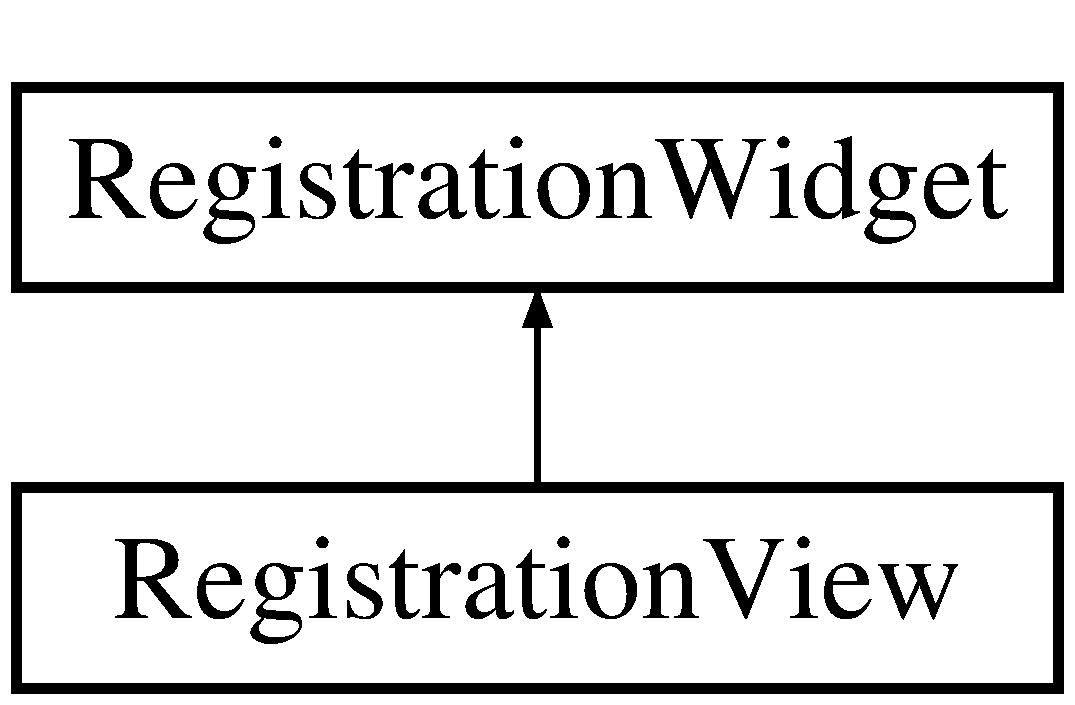
\includegraphics[height=2.000000cm]{class_registration_view}
\end{center}
\end{figure}
\subsection*{Public Member Functions}
\begin{DoxyCompactItemize}
\item 
\hyperlink{class_registration_view_a3848c621b2e4176060293f6f80c16fa7}{Registration\+View} (\hyperlink{class_session}{Session} \&session, Wt\+::\+Auth\+::\+Auth\+Widget $\ast$auth\+Widget=0)
\item 
virtual Wt\+::\+W\+Widget $\ast$ \hyperlink{class_registration_view_ae2a0695f816ba4d0f9845b5da6539b34}{create\+Form\+Widget} (Wt\+::\+W\+Form\+Model\+::\+Field field)
\end{DoxyCompactItemize}
\subsection*{Protected Member Functions}
\begin{DoxyCompactItemize}
\item 
virtual bool \hyperlink{class_registration_view_abff4da7c898c36d81a8af6718840d27e}{validate} ()
\item 
virtual void \hyperlink{class_registration_view_a2e048b6c3103bedacd90a33f6664512b}{register\+User\+Details} (Wt\+::\+Auth\+::\+User \&user)
\end{DoxyCompactItemize}
\subsection*{Private Attributes}
\begin{DoxyCompactItemize}
\item 
\hyperlink{class_session}{Session} \& \hyperlink{class_registration_view_aef6dd993c0249d9fe34d6a32f12a4694}{session\+\_\+}
\item 
\hyperlink{class_user_details_model}{User\+Details\+Model} $\ast$ \hyperlink{class_registration_view_a95789059816b6c1cabe07b683ad51f61}{details\+Model\+\_\+}
\end{DoxyCompactItemize}


\subsection{Constructor \& Destructor Documentation}
\mbox{\Hypertarget{class_registration_view_a3848c621b2e4176060293f6f80c16fa7}\label{class_registration_view_a3848c621b2e4176060293f6f80c16fa7}} 
\index{Registration\+View@{Registration\+View}!Registration\+View@{Registration\+View}}
\index{Registration\+View@{Registration\+View}!Registration\+View@{Registration\+View}}
\subsubsection{\texorpdfstring{Registration\+View()}{RegistrationView()}}
{\footnotesize\ttfamily Registration\+View\+::\+Registration\+View (\begin{DoxyParamCaption}\item[{\hyperlink{class_session}{Session} \&}]{session,  }\item[{Wt\+::\+Auth\+::\+Auth\+Widget $\ast$}]{auth\+Widget = {\ttfamily 0} }\end{DoxyParamCaption})}



\subsection{Member Function Documentation}
\mbox{\Hypertarget{class_registration_view_ae2a0695f816ba4d0f9845b5da6539b34}\label{class_registration_view_ae2a0695f816ba4d0f9845b5da6539b34}} 
\index{Registration\+View@{Registration\+View}!create\+Form\+Widget@{create\+Form\+Widget}}
\index{create\+Form\+Widget@{create\+Form\+Widget}!Registration\+View@{Registration\+View}}
\subsubsection{\texorpdfstring{create\+Form\+Widget()}{createFormWidget()}}
{\footnotesize\ttfamily Wt\+::\+W\+Widget $\ast$ Registration\+View\+::create\+Form\+Widget (\begin{DoxyParamCaption}\item[{Wt\+::\+W\+Form\+Model\+::\+Field}]{field }\end{DoxyParamCaption})\hspace{0.3cm}{\ttfamily [virtual]}}

\mbox{\Hypertarget{class_registration_view_a2e048b6c3103bedacd90a33f6664512b}\label{class_registration_view_a2e048b6c3103bedacd90a33f6664512b}} 
\index{Registration\+View@{Registration\+View}!register\+User\+Details@{register\+User\+Details}}
\index{register\+User\+Details@{register\+User\+Details}!Registration\+View@{Registration\+View}}
\subsubsection{\texorpdfstring{register\+User\+Details()}{registerUserDetails()}}
{\footnotesize\ttfamily void Registration\+View\+::register\+User\+Details (\begin{DoxyParamCaption}\item[{Wt\+::\+Auth\+::\+User \&}]{user }\end{DoxyParamCaption})\hspace{0.3cm}{\ttfamily [protected]}, {\ttfamily [virtual]}}

\mbox{\Hypertarget{class_registration_view_abff4da7c898c36d81a8af6718840d27e}\label{class_registration_view_abff4da7c898c36d81a8af6718840d27e}} 
\index{Registration\+View@{Registration\+View}!validate@{validate}}
\index{validate@{validate}!Registration\+View@{Registration\+View}}
\subsubsection{\texorpdfstring{validate()}{validate()}}
{\footnotesize\ttfamily bool Registration\+View\+::validate (\begin{DoxyParamCaption}{ }\end{DoxyParamCaption})\hspace{0.3cm}{\ttfamily [protected]}, {\ttfamily [virtual]}}



\subsection{Member Data Documentation}
\mbox{\Hypertarget{class_registration_view_a95789059816b6c1cabe07b683ad51f61}\label{class_registration_view_a95789059816b6c1cabe07b683ad51f61}} 
\index{Registration\+View@{Registration\+View}!details\+Model\+\_\+@{details\+Model\+\_\+}}
\index{details\+Model\+\_\+@{details\+Model\+\_\+}!Registration\+View@{Registration\+View}}
\subsubsection{\texorpdfstring{details\+Model\+\_\+}{detailsModel\_}}
{\footnotesize\ttfamily \hyperlink{class_user_details_model}{User\+Details\+Model}$\ast$ Registration\+View\+::details\+Model\+\_\+\hspace{0.3cm}{\ttfamily [private]}}

\mbox{\Hypertarget{class_registration_view_aef6dd993c0249d9fe34d6a32f12a4694}\label{class_registration_view_aef6dd993c0249d9fe34d6a32f12a4694}} 
\index{Registration\+View@{Registration\+View}!session\+\_\+@{session\+\_\+}}
\index{session\+\_\+@{session\+\_\+}!Registration\+View@{Registration\+View}}
\subsubsection{\texorpdfstring{session\+\_\+}{session\_}}
{\footnotesize\ttfamily \hyperlink{class_session}{Session}\& Registration\+View\+::session\+\_\+\hspace{0.3cm}{\ttfamily [private]}}



The documentation for this class was generated from the following files\+:\begin{DoxyCompactItemize}
\item 
\hyperlink{_registration_view_8h}{Registration\+View.\+h}\item 
\hyperlink{_registration_view_8_c}{Registration\+View.\+C}\end{DoxyCompactItemize}

\hypertarget{class_scheduler_control_widget}{}\section{Scheduler\+Control\+Widget Class Reference}
\label{class_scheduler_control_widget}\index{Scheduler\+Control\+Widget@{Scheduler\+Control\+Widget}}


{\ttfamily \#include $<$Scheduler\+Control.\+h$>$}

Inheritance diagram for Scheduler\+Control\+Widget\+:\begin{figure}[H]
\begin{center}
\leavevmode
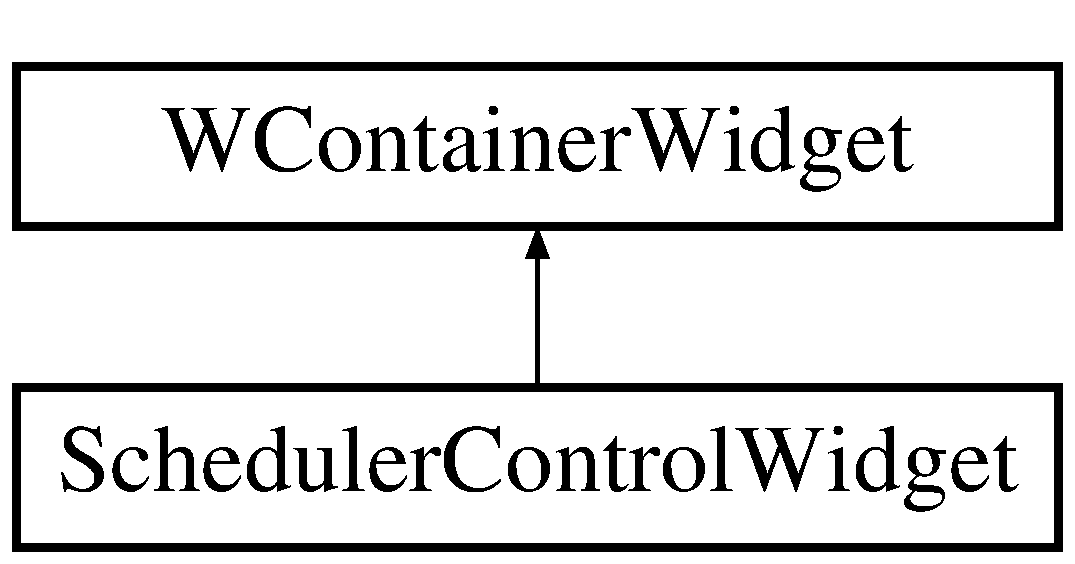
\includegraphics[height=2.000000cm]{class_scheduler_control_widget}
\end{center}
\end{figure}
\subsection*{Public Member Functions}
\begin{DoxyCompactItemize}
\item 
\hyperlink{class_scheduler_control_widget_a88824ef71ef84e9e5bdb85ab3f4f9952}{Scheduler\+Control\+Widget} (\hyperlink{class_session}{Session} $\ast$session, Wt\+::\+W\+Container\+Widget $\ast$parent=0)
\item 
void \hyperlink{class_scheduler_control_widget_acca1c74b4dc6fa16c079da6b2e946f4b}{update} ()
\end{DoxyCompactItemize}
\subsection*{Private Member Functions}
\begin{DoxyCompactItemize}
\item 
void \hyperlink{class_scheduler_control_widget_ad703c8e5f15d4ebaaeeed55450d984f4}{on} ()
\item 
void \hyperlink{class_scheduler_control_widget_a4a88b0dd02bde7d3b77f6dc1b907dd46}{off} ()
\item 
void \hyperlink{class_scheduler_control_widget_ac94a6b7fffc3ad41f47d4f3055278a9f}{hue} ()
\item 
void \hyperlink{class_scheduler_control_widget_abfb0dd8c7d7ef3a7bef6f291cfcf5bdd}{bright} ()
\item 
void \hyperlink{class_scheduler_control_widget_a43834db378ceb523fa8c0ee7defea951}{sat} ()
\item 
void \hyperlink{class_scheduler_control_widget_aafbad4eb5ff9cf0d0d311dc805df49c1}{name} ()
\item 
void \hyperlink{class_scheduler_control_widget_a469057104fb5ce001a248a210fb90878}{transition} ()
\item 
void \hyperlink{class_scheduler_control_widget_a9b2cb5e76ca840104928a5016741cd4c}{handle\+Http\+Response} (boost\+::system\+::error\+\_\+code err, const Wt\+::\+Http\+::\+Message \&response)
\item 
void \hyperlink{class_scheduler_control_widget_a6adf770a92a199b5557ffabc0a6dc6a8}{handle\+Http\+Response\+Name} (boost\+::system\+::error\+\_\+code err, const Wt\+::\+Http\+::\+Message \&response)
\item 
void \hyperlink{class_scheduler_control_widget_a608cf1aa0348a5a9db24b199136beff6}{handle\+Http\+Response\+V\+O\+ID} (boost\+::system\+::error\+\_\+code err, const Wt\+::\+Http\+::\+Message \&response)
\item 
Wt\+::\+Http\+::\+Client $\ast$ \hyperlink{class_scheduler_control_widget_ace95dce867b19128d2ac1d9b7f6af2df}{connect} ()
\item 
void \hyperlink{class_scheduler_control_widget_ad7c66eaaf55c7ca61126e85681288f10}{light\+One} ()
\item 
void \hyperlink{class_scheduler_control_widget_a952c792697ead97f959faaef2f9344cd}{light\+Two} ()
\item 
void \hyperlink{class_scheduler_control_widget_a818b2e33f2e9cfc0fa466a6681d581fc}{light\+Three} ()
\item 
void \hyperlink{class_scheduler_control_widget_a3f4447117c1338a01e90c582f2666713}{return\+Bridge} ()
\item 
void \hyperlink{class_scheduler_control_widget_ad6aba10b47fa2f8c57c08bc4171a2a94}{change\+Date} ()
\item 
void \hyperlink{class_scheduler_control_widget_afbf344c96240de973c3f4bdc2f49c23c}{create\+Schedule} ()
\item 
void \hyperlink{class_scheduler_control_widget_ab0d3185086154680e558a7a9eaa978aa}{change\+Hour} ()
\item 
void \hyperlink{class_scheduler_control_widget_a9cdf27c0acc6d8f84c400b1ac8b29995}{change\+Min} ()
\item 
void \hyperlink{class_scheduler_control_widget_a5d24965e21d773cf4013f1af9438b990}{change\+Sec} ()
\item 
std\+::string \hyperlink{class_scheduler_control_widget_a59d6549a621edc590f321292a1946ee2}{create\+Body\+Message} ()
\item 
std\+::string \hyperlink{class_scheduler_control_widget_aa5aa766921972a9d00818deccddfff33}{create\+Post\+Message} ()
\item 
std\+::string \hyperlink{class_scheduler_control_widget_afeebc21f1fc76100e475b6c75bb97034}{create\+Date\+Time} ()
\end{DoxyCompactItemize}
\subsection*{Private Attributes}
\begin{DoxyCompactItemize}
\item 
\hyperlink{class_session}{Session} $\ast$ \hyperlink{class_scheduler_control_widget_a288a93234db52da45170f791c9014459}{session\+\_\+}
\item 
Wt\+::\+W\+Line\+Edit $\ast$ \hyperlink{class_scheduler_control_widget_afb6d2313419723521e39ee1d778efc3c}{name\+Edit\+\_\+}
\item 
Wt\+::\+W\+Line\+Edit $\ast$ \hyperlink{class_scheduler_control_widget_aeaf9ad2492fe9fcbf2133d589a86c0a3}{hue\+Edit\+\_\+}
\item 
Wt\+::\+W\+Slider $\ast$ \hyperlink{class_scheduler_control_widget_a7d6fcaadf1b4c1b5dc2463ed83aed2e3}{sat\+Scale\+Slider\+\_\+}
\item 
Wt\+::\+W\+Slider $\ast$ \hyperlink{class_scheduler_control_widget_af20be6b36f21400890eb6f09169bc3ac}{bri\+Scale\+Slider\+\_\+}
\item 
Wt\+::\+W\+Slider $\ast$ \hyperlink{class_scheduler_control_widget_a51a54fca3870348a0de577e7a10841c2}{hue\+Scale\+Slider\+\_\+}
\item 
Wt\+::\+W\+Slider $\ast$ \hyperlink{class_scheduler_control_widget_af33baa9348cda84a1b330fa098304801}{transition\+Scale\+Slider\+\_\+}
\item 
Wt\+::\+W\+Calendar $\ast$ \hyperlink{class_scheduler_control_widget_a09cb3b1c1b563ac1f93ffe6f7d562d1d}{calendar\+\_\+}
\item 
Wt\+::\+W\+Combo\+Box $\ast$ \hyperlink{class_scheduler_control_widget_a23c3048a8008ec1296b8fbc660c7b956}{hour\+Input\+\_\+}
\item 
Wt\+::\+W\+Combo\+Box $\ast$ \hyperlink{class_scheduler_control_widget_a254d87a1ab315532cc13c179ab8ea8e2}{min\+Input\+\_\+}
\item 
Wt\+::\+W\+Combo\+Box $\ast$ \hyperlink{class_scheduler_control_widget_a3f522e0b3b6e3c2dee44230dcec56f03}{sec\+Input\+\_\+}
\item 
Wt\+::\+W\+Combo\+Box $\ast$ \hyperlink{class_scheduler_control_widget_a962a04d3d4638fce987915b227301ad6}{am\+Selector\+\_\+}
\item 
Wt\+::\+W\+Text $\ast$ \hyperlink{class_scheduler_control_widget_a0ab7ae0a5695085094ddb2da0f80ca83}{one\+Light\+\_\+}
\item 
Wt\+::\+W\+Text $\ast$ \hyperlink{class_scheduler_control_widget_a3811f8b85a16cae05f9ec9630f395349}{two\+Light\+\_\+}
\item 
Wt\+::\+W\+Text $\ast$ \hyperlink{class_scheduler_control_widget_a9cba1fa625c734f4dbbf11d8a0218004}{three\+Light\+\_\+}
\item 
Wt\+::\+W\+Text $\ast$ \hyperlink{class_scheduler_control_widget_a9e38298e1acc9bcee2052d62b9aad527}{change\+\_\+}
\item 
Wt\+::\+W\+Text $\ast$ \hyperlink{class_scheduler_control_widget_af92e4f56cb39cd45150c947babd5c0a7}{light\+\_\+}
\item 
Wt\+::\+W\+Text $\ast$ \hyperlink{class_scheduler_control_widget_a156653c34485d3435d079593968e3dba}{date\+Select\+\_\+}
\item 
std\+::string \hyperlink{class_scheduler_control_widget_a1623869aaefe631dba02f2533033d2a2}{current\+Light} = \char`\"{}0\char`\"{}
\item 
std\+::string \hyperlink{class_scheduler_control_widget_a320557ef7428e36682b21d9ad3b877ba}{ip} = \char`\"{}\char`\"{}
\item 
std\+::string \hyperlink{class_scheduler_control_widget_af73ee1b98fb7944ae193d5e880a59f31}{user\+ID} = \char`\"{}\char`\"{}
\item 
std\+::string \hyperlink{class_scheduler_control_widget_add76e052c3bbb0bedfef92ff5121e8b0}{port} = \char`\"{}\char`\"{}
\item 
\hyperlink{structdate_time}{date\+Time} \hyperlink{class_scheduler_control_widget_a79515f4694dac8b92af2582498654ec4}{input\+Data}
\end{DoxyCompactItemize}


\subsection{Constructor \& Destructor Documentation}
\mbox{\Hypertarget{class_scheduler_control_widget_a88824ef71ef84e9e5bdb85ab3f4f9952}\label{class_scheduler_control_widget_a88824ef71ef84e9e5bdb85ab3f4f9952}} 
\index{Scheduler\+Control\+Widget@{Scheduler\+Control\+Widget}!Scheduler\+Control\+Widget@{Scheduler\+Control\+Widget}}
\index{Scheduler\+Control\+Widget@{Scheduler\+Control\+Widget}!Scheduler\+Control\+Widget@{Scheduler\+Control\+Widget}}
\subsubsection{\texorpdfstring{Scheduler\+Control\+Widget()}{SchedulerControlWidget()}}
{\footnotesize\ttfamily Scheduler\+Control\+Widget\+::\+Scheduler\+Control\+Widget (\begin{DoxyParamCaption}\item[{\hyperlink{class_session}{Session} $\ast$}]{session,  }\item[{Wt\+::\+W\+Container\+Widget $\ast$}]{parent = {\ttfamily 0} }\end{DoxyParamCaption})}



\subsection{Member Function Documentation}
\mbox{\Hypertarget{class_scheduler_control_widget_abfb0dd8c7d7ef3a7bef6f291cfcf5bdd}\label{class_scheduler_control_widget_abfb0dd8c7d7ef3a7bef6f291cfcf5bdd}} 
\index{Scheduler\+Control\+Widget@{Scheduler\+Control\+Widget}!bright@{bright}}
\index{bright@{bright}!Scheduler\+Control\+Widget@{Scheduler\+Control\+Widget}}
\subsubsection{\texorpdfstring{bright()}{bright()}}
{\footnotesize\ttfamily void Scheduler\+Control\+Widget\+::bright (\begin{DoxyParamCaption}{ }\end{DoxyParamCaption})\hspace{0.3cm}{\ttfamily [private]}}

\mbox{\Hypertarget{class_scheduler_control_widget_ad6aba10b47fa2f8c57c08bc4171a2a94}\label{class_scheduler_control_widget_ad6aba10b47fa2f8c57c08bc4171a2a94}} 
\index{Scheduler\+Control\+Widget@{Scheduler\+Control\+Widget}!change\+Date@{change\+Date}}
\index{change\+Date@{change\+Date}!Scheduler\+Control\+Widget@{Scheduler\+Control\+Widget}}
\subsubsection{\texorpdfstring{change\+Date()}{changeDate()}}
{\footnotesize\ttfamily void Scheduler\+Control\+Widget\+::change\+Date (\begin{DoxyParamCaption}{ }\end{DoxyParamCaption})\hspace{0.3cm}{\ttfamily [private]}}

\mbox{\Hypertarget{class_scheduler_control_widget_ab0d3185086154680e558a7a9eaa978aa}\label{class_scheduler_control_widget_ab0d3185086154680e558a7a9eaa978aa}} 
\index{Scheduler\+Control\+Widget@{Scheduler\+Control\+Widget}!change\+Hour@{change\+Hour}}
\index{change\+Hour@{change\+Hour}!Scheduler\+Control\+Widget@{Scheduler\+Control\+Widget}}
\subsubsection{\texorpdfstring{change\+Hour()}{changeHour()}}
{\footnotesize\ttfamily void Scheduler\+Control\+Widget\+::change\+Hour (\begin{DoxyParamCaption}{ }\end{DoxyParamCaption})\hspace{0.3cm}{\ttfamily [private]}}

\mbox{\Hypertarget{class_scheduler_control_widget_a9cdf27c0acc6d8f84c400b1ac8b29995}\label{class_scheduler_control_widget_a9cdf27c0acc6d8f84c400b1ac8b29995}} 
\index{Scheduler\+Control\+Widget@{Scheduler\+Control\+Widget}!change\+Min@{change\+Min}}
\index{change\+Min@{change\+Min}!Scheduler\+Control\+Widget@{Scheduler\+Control\+Widget}}
\subsubsection{\texorpdfstring{change\+Min()}{changeMin()}}
{\footnotesize\ttfamily void Scheduler\+Control\+Widget\+::change\+Min (\begin{DoxyParamCaption}{ }\end{DoxyParamCaption})\hspace{0.3cm}{\ttfamily [private]}}

\mbox{\Hypertarget{class_scheduler_control_widget_a5d24965e21d773cf4013f1af9438b990}\label{class_scheduler_control_widget_a5d24965e21d773cf4013f1af9438b990}} 
\index{Scheduler\+Control\+Widget@{Scheduler\+Control\+Widget}!change\+Sec@{change\+Sec}}
\index{change\+Sec@{change\+Sec}!Scheduler\+Control\+Widget@{Scheduler\+Control\+Widget}}
\subsubsection{\texorpdfstring{change\+Sec()}{changeSec()}}
{\footnotesize\ttfamily void Scheduler\+Control\+Widget\+::change\+Sec (\begin{DoxyParamCaption}{ }\end{DoxyParamCaption})\hspace{0.3cm}{\ttfamily [private]}}

\mbox{\Hypertarget{class_scheduler_control_widget_ace95dce867b19128d2ac1d9b7f6af2df}\label{class_scheduler_control_widget_ace95dce867b19128d2ac1d9b7f6af2df}} 
\index{Scheduler\+Control\+Widget@{Scheduler\+Control\+Widget}!connect@{connect}}
\index{connect@{connect}!Scheduler\+Control\+Widget@{Scheduler\+Control\+Widget}}
\subsubsection{\texorpdfstring{connect()}{connect()}}
{\footnotesize\ttfamily Http\+::\+Client $\ast$ Scheduler\+Control\+Widget\+::connect (\begin{DoxyParamCaption}{ }\end{DoxyParamCaption})\hspace{0.3cm}{\ttfamily [private]}}

\mbox{\Hypertarget{class_scheduler_control_widget_a59d6549a621edc590f321292a1946ee2}\label{class_scheduler_control_widget_a59d6549a621edc590f321292a1946ee2}} 
\index{Scheduler\+Control\+Widget@{Scheduler\+Control\+Widget}!create\+Body\+Message@{create\+Body\+Message}}
\index{create\+Body\+Message@{create\+Body\+Message}!Scheduler\+Control\+Widget@{Scheduler\+Control\+Widget}}
\subsubsection{\texorpdfstring{create\+Body\+Message()}{createBodyMessage()}}
{\footnotesize\ttfamily std\+::string Scheduler\+Control\+Widget\+::create\+Body\+Message (\begin{DoxyParamCaption}{ }\end{DoxyParamCaption})\hspace{0.3cm}{\ttfamily [private]}}

\mbox{\Hypertarget{class_scheduler_control_widget_afeebc21f1fc76100e475b6c75bb97034}\label{class_scheduler_control_widget_afeebc21f1fc76100e475b6c75bb97034}} 
\index{Scheduler\+Control\+Widget@{Scheduler\+Control\+Widget}!create\+Date\+Time@{create\+Date\+Time}}
\index{create\+Date\+Time@{create\+Date\+Time}!Scheduler\+Control\+Widget@{Scheduler\+Control\+Widget}}
\subsubsection{\texorpdfstring{create\+Date\+Time()}{createDateTime()}}
{\footnotesize\ttfamily std\+::string Scheduler\+Control\+Widget\+::create\+Date\+Time (\begin{DoxyParamCaption}{ }\end{DoxyParamCaption})\hspace{0.3cm}{\ttfamily [private]}}

\mbox{\Hypertarget{class_scheduler_control_widget_aa5aa766921972a9d00818deccddfff33}\label{class_scheduler_control_widget_aa5aa766921972a9d00818deccddfff33}} 
\index{Scheduler\+Control\+Widget@{Scheduler\+Control\+Widget}!create\+Post\+Message@{create\+Post\+Message}}
\index{create\+Post\+Message@{create\+Post\+Message}!Scheduler\+Control\+Widget@{Scheduler\+Control\+Widget}}
\subsubsection{\texorpdfstring{create\+Post\+Message()}{createPostMessage()}}
{\footnotesize\ttfamily std\+::string Scheduler\+Control\+Widget\+::create\+Post\+Message (\begin{DoxyParamCaption}{ }\end{DoxyParamCaption})\hspace{0.3cm}{\ttfamily [private]}}

\mbox{\Hypertarget{class_scheduler_control_widget_afbf344c96240de973c3f4bdc2f49c23c}\label{class_scheduler_control_widget_afbf344c96240de973c3f4bdc2f49c23c}} 
\index{Scheduler\+Control\+Widget@{Scheduler\+Control\+Widget}!create\+Schedule@{create\+Schedule}}
\index{create\+Schedule@{create\+Schedule}!Scheduler\+Control\+Widget@{Scheduler\+Control\+Widget}}
\subsubsection{\texorpdfstring{create\+Schedule()}{createSchedule()}}
{\footnotesize\ttfamily void Scheduler\+Control\+Widget\+::create\+Schedule (\begin{DoxyParamCaption}{ }\end{DoxyParamCaption})\hspace{0.3cm}{\ttfamily [private]}}

\mbox{\Hypertarget{class_scheduler_control_widget_a9b2cb5e76ca840104928a5016741cd4c}\label{class_scheduler_control_widget_a9b2cb5e76ca840104928a5016741cd4c}} 
\index{Scheduler\+Control\+Widget@{Scheduler\+Control\+Widget}!handle\+Http\+Response@{handle\+Http\+Response}}
\index{handle\+Http\+Response@{handle\+Http\+Response}!Scheduler\+Control\+Widget@{Scheduler\+Control\+Widget}}
\subsubsection{\texorpdfstring{handle\+Http\+Response()}{handleHttpResponse()}}
{\footnotesize\ttfamily void Scheduler\+Control\+Widget\+::handle\+Http\+Response (\begin{DoxyParamCaption}\item[{boost\+::system\+::error\+\_\+code}]{err,  }\item[{const Wt\+::\+Http\+::\+Message \&}]{response }\end{DoxyParamCaption})\hspace{0.3cm}{\ttfamily [private]}}

\mbox{\Hypertarget{class_scheduler_control_widget_a6adf770a92a199b5557ffabc0a6dc6a8}\label{class_scheduler_control_widget_a6adf770a92a199b5557ffabc0a6dc6a8}} 
\index{Scheduler\+Control\+Widget@{Scheduler\+Control\+Widget}!handle\+Http\+Response\+Name@{handle\+Http\+Response\+Name}}
\index{handle\+Http\+Response\+Name@{handle\+Http\+Response\+Name}!Scheduler\+Control\+Widget@{Scheduler\+Control\+Widget}}
\subsubsection{\texorpdfstring{handle\+Http\+Response\+Name()}{handleHttpResponseName()}}
{\footnotesize\ttfamily void Scheduler\+Control\+Widget\+::handle\+Http\+Response\+Name (\begin{DoxyParamCaption}\item[{boost\+::system\+::error\+\_\+code}]{err,  }\item[{const Wt\+::\+Http\+::\+Message \&}]{response }\end{DoxyParamCaption})\hspace{0.3cm}{\ttfamily [private]}}

\mbox{\Hypertarget{class_scheduler_control_widget_a608cf1aa0348a5a9db24b199136beff6}\label{class_scheduler_control_widget_a608cf1aa0348a5a9db24b199136beff6}} 
\index{Scheduler\+Control\+Widget@{Scheduler\+Control\+Widget}!handle\+Http\+Response\+V\+O\+ID@{handle\+Http\+Response\+V\+O\+ID}}
\index{handle\+Http\+Response\+V\+O\+ID@{handle\+Http\+Response\+V\+O\+ID}!Scheduler\+Control\+Widget@{Scheduler\+Control\+Widget}}
\subsubsection{\texorpdfstring{handle\+Http\+Response\+V\+O\+I\+D()}{handleHttpResponseVOID()}}
{\footnotesize\ttfamily void Scheduler\+Control\+Widget\+::handle\+Http\+Response\+V\+O\+ID (\begin{DoxyParamCaption}\item[{boost\+::system\+::error\+\_\+code}]{err,  }\item[{const Wt\+::\+Http\+::\+Message \&}]{response }\end{DoxyParamCaption})\hspace{0.3cm}{\ttfamily [private]}}

\mbox{\Hypertarget{class_scheduler_control_widget_ac94a6b7fffc3ad41f47d4f3055278a9f}\label{class_scheduler_control_widget_ac94a6b7fffc3ad41f47d4f3055278a9f}} 
\index{Scheduler\+Control\+Widget@{Scheduler\+Control\+Widget}!hue@{hue}}
\index{hue@{hue}!Scheduler\+Control\+Widget@{Scheduler\+Control\+Widget}}
\subsubsection{\texorpdfstring{hue()}{hue()}}
{\footnotesize\ttfamily void Scheduler\+Control\+Widget\+::hue (\begin{DoxyParamCaption}{ }\end{DoxyParamCaption})\hspace{0.3cm}{\ttfamily [private]}}

\mbox{\Hypertarget{class_scheduler_control_widget_ad7c66eaaf55c7ca61126e85681288f10}\label{class_scheduler_control_widget_ad7c66eaaf55c7ca61126e85681288f10}} 
\index{Scheduler\+Control\+Widget@{Scheduler\+Control\+Widget}!light\+One@{light\+One}}
\index{light\+One@{light\+One}!Scheduler\+Control\+Widget@{Scheduler\+Control\+Widget}}
\subsubsection{\texorpdfstring{light\+One()}{lightOne()}}
{\footnotesize\ttfamily void Scheduler\+Control\+Widget\+::light\+One (\begin{DoxyParamCaption}{ }\end{DoxyParamCaption})\hspace{0.3cm}{\ttfamily [private]}}

\mbox{\Hypertarget{class_scheduler_control_widget_a818b2e33f2e9cfc0fa466a6681d581fc}\label{class_scheduler_control_widget_a818b2e33f2e9cfc0fa466a6681d581fc}} 
\index{Scheduler\+Control\+Widget@{Scheduler\+Control\+Widget}!light\+Three@{light\+Three}}
\index{light\+Three@{light\+Three}!Scheduler\+Control\+Widget@{Scheduler\+Control\+Widget}}
\subsubsection{\texorpdfstring{light\+Three()}{lightThree()}}
{\footnotesize\ttfamily void Scheduler\+Control\+Widget\+::light\+Three (\begin{DoxyParamCaption}{ }\end{DoxyParamCaption})\hspace{0.3cm}{\ttfamily [private]}}

\mbox{\Hypertarget{class_scheduler_control_widget_a952c792697ead97f959faaef2f9344cd}\label{class_scheduler_control_widget_a952c792697ead97f959faaef2f9344cd}} 
\index{Scheduler\+Control\+Widget@{Scheduler\+Control\+Widget}!light\+Two@{light\+Two}}
\index{light\+Two@{light\+Two}!Scheduler\+Control\+Widget@{Scheduler\+Control\+Widget}}
\subsubsection{\texorpdfstring{light\+Two()}{lightTwo()}}
{\footnotesize\ttfamily void Scheduler\+Control\+Widget\+::light\+Two (\begin{DoxyParamCaption}{ }\end{DoxyParamCaption})\hspace{0.3cm}{\ttfamily [private]}}

\mbox{\Hypertarget{class_scheduler_control_widget_aafbad4eb5ff9cf0d0d311dc805df49c1}\label{class_scheduler_control_widget_aafbad4eb5ff9cf0d0d311dc805df49c1}} 
\index{Scheduler\+Control\+Widget@{Scheduler\+Control\+Widget}!name@{name}}
\index{name@{name}!Scheduler\+Control\+Widget@{Scheduler\+Control\+Widget}}
\subsubsection{\texorpdfstring{name()}{name()}}
{\footnotesize\ttfamily void Scheduler\+Control\+Widget\+::name (\begin{DoxyParamCaption}{ }\end{DoxyParamCaption})\hspace{0.3cm}{\ttfamily [private]}}

\mbox{\Hypertarget{class_scheduler_control_widget_a4a88b0dd02bde7d3b77f6dc1b907dd46}\label{class_scheduler_control_widget_a4a88b0dd02bde7d3b77f6dc1b907dd46}} 
\index{Scheduler\+Control\+Widget@{Scheduler\+Control\+Widget}!off@{off}}
\index{off@{off}!Scheduler\+Control\+Widget@{Scheduler\+Control\+Widget}}
\subsubsection{\texorpdfstring{off()}{off()}}
{\footnotesize\ttfamily void Scheduler\+Control\+Widget\+::off (\begin{DoxyParamCaption}{ }\end{DoxyParamCaption})\hspace{0.3cm}{\ttfamily [private]}}

\mbox{\Hypertarget{class_scheduler_control_widget_ad703c8e5f15d4ebaaeeed55450d984f4}\label{class_scheduler_control_widget_ad703c8e5f15d4ebaaeeed55450d984f4}} 
\index{Scheduler\+Control\+Widget@{Scheduler\+Control\+Widget}!on@{on}}
\index{on@{on}!Scheduler\+Control\+Widget@{Scheduler\+Control\+Widget}}
\subsubsection{\texorpdfstring{on()}{on()}}
{\footnotesize\ttfamily void Scheduler\+Control\+Widget\+::on (\begin{DoxyParamCaption}{ }\end{DoxyParamCaption})\hspace{0.3cm}{\ttfamily [private]}}

\mbox{\Hypertarget{class_scheduler_control_widget_a3f4447117c1338a01e90c582f2666713}\label{class_scheduler_control_widget_a3f4447117c1338a01e90c582f2666713}} 
\index{Scheduler\+Control\+Widget@{Scheduler\+Control\+Widget}!return\+Bridge@{return\+Bridge}}
\index{return\+Bridge@{return\+Bridge}!Scheduler\+Control\+Widget@{Scheduler\+Control\+Widget}}
\subsubsection{\texorpdfstring{return\+Bridge()}{returnBridge()}}
{\footnotesize\ttfamily void Scheduler\+Control\+Widget\+::return\+Bridge (\begin{DoxyParamCaption}{ }\end{DoxyParamCaption})\hspace{0.3cm}{\ttfamily [private]}}

\mbox{\Hypertarget{class_scheduler_control_widget_a43834db378ceb523fa8c0ee7defea951}\label{class_scheduler_control_widget_a43834db378ceb523fa8c0ee7defea951}} 
\index{Scheduler\+Control\+Widget@{Scheduler\+Control\+Widget}!sat@{sat}}
\index{sat@{sat}!Scheduler\+Control\+Widget@{Scheduler\+Control\+Widget}}
\subsubsection{\texorpdfstring{sat()}{sat()}}
{\footnotesize\ttfamily void Scheduler\+Control\+Widget\+::sat (\begin{DoxyParamCaption}{ }\end{DoxyParamCaption})\hspace{0.3cm}{\ttfamily [private]}}

\mbox{\Hypertarget{class_scheduler_control_widget_a469057104fb5ce001a248a210fb90878}\label{class_scheduler_control_widget_a469057104fb5ce001a248a210fb90878}} 
\index{Scheduler\+Control\+Widget@{Scheduler\+Control\+Widget}!transition@{transition}}
\index{transition@{transition}!Scheduler\+Control\+Widget@{Scheduler\+Control\+Widget}}
\subsubsection{\texorpdfstring{transition()}{transition()}}
{\footnotesize\ttfamily void Scheduler\+Control\+Widget\+::transition (\begin{DoxyParamCaption}{ }\end{DoxyParamCaption})\hspace{0.3cm}{\ttfamily [private]}}

\mbox{\Hypertarget{class_scheduler_control_widget_acca1c74b4dc6fa16c079da6b2e946f4b}\label{class_scheduler_control_widget_acca1c74b4dc6fa16c079da6b2e946f4b}} 
\index{Scheduler\+Control\+Widget@{Scheduler\+Control\+Widget}!update@{update}}
\index{update@{update}!Scheduler\+Control\+Widget@{Scheduler\+Control\+Widget}}
\subsubsection{\texorpdfstring{update()}{update()}}
{\footnotesize\ttfamily void Scheduler\+Control\+Widget\+::update (\begin{DoxyParamCaption}{ }\end{DoxyParamCaption})}



\subsection{Member Data Documentation}
\mbox{\Hypertarget{class_scheduler_control_widget_a962a04d3d4638fce987915b227301ad6}\label{class_scheduler_control_widget_a962a04d3d4638fce987915b227301ad6}} 
\index{Scheduler\+Control\+Widget@{Scheduler\+Control\+Widget}!am\+Selector\+\_\+@{am\+Selector\+\_\+}}
\index{am\+Selector\+\_\+@{am\+Selector\+\_\+}!Scheduler\+Control\+Widget@{Scheduler\+Control\+Widget}}
\subsubsection{\texorpdfstring{am\+Selector\+\_\+}{amSelector\_}}
{\footnotesize\ttfamily Wt\+::\+W\+Combo\+Box$\ast$ Scheduler\+Control\+Widget\+::am\+Selector\+\_\+\hspace{0.3cm}{\ttfamily [private]}}

\mbox{\Hypertarget{class_scheduler_control_widget_af20be6b36f21400890eb6f09169bc3ac}\label{class_scheduler_control_widget_af20be6b36f21400890eb6f09169bc3ac}} 
\index{Scheduler\+Control\+Widget@{Scheduler\+Control\+Widget}!bri\+Scale\+Slider\+\_\+@{bri\+Scale\+Slider\+\_\+}}
\index{bri\+Scale\+Slider\+\_\+@{bri\+Scale\+Slider\+\_\+}!Scheduler\+Control\+Widget@{Scheduler\+Control\+Widget}}
\subsubsection{\texorpdfstring{bri\+Scale\+Slider\+\_\+}{briScaleSlider\_}}
{\footnotesize\ttfamily Wt\+::\+W\+Slider$\ast$ Scheduler\+Control\+Widget\+::bri\+Scale\+Slider\+\_\+\hspace{0.3cm}{\ttfamily [private]}}

\mbox{\Hypertarget{class_scheduler_control_widget_a09cb3b1c1b563ac1f93ffe6f7d562d1d}\label{class_scheduler_control_widget_a09cb3b1c1b563ac1f93ffe6f7d562d1d}} 
\index{Scheduler\+Control\+Widget@{Scheduler\+Control\+Widget}!calendar\+\_\+@{calendar\+\_\+}}
\index{calendar\+\_\+@{calendar\+\_\+}!Scheduler\+Control\+Widget@{Scheduler\+Control\+Widget}}
\subsubsection{\texorpdfstring{calendar\+\_\+}{calendar\_}}
{\footnotesize\ttfamily Wt\+::\+W\+Calendar$\ast$ Scheduler\+Control\+Widget\+::calendar\+\_\+\hspace{0.3cm}{\ttfamily [private]}}

\mbox{\Hypertarget{class_scheduler_control_widget_a9e38298e1acc9bcee2052d62b9aad527}\label{class_scheduler_control_widget_a9e38298e1acc9bcee2052d62b9aad527}} 
\index{Scheduler\+Control\+Widget@{Scheduler\+Control\+Widget}!change\+\_\+@{change\+\_\+}}
\index{change\+\_\+@{change\+\_\+}!Scheduler\+Control\+Widget@{Scheduler\+Control\+Widget}}
\subsubsection{\texorpdfstring{change\+\_\+}{change\_}}
{\footnotesize\ttfamily Wt\+::\+W\+Text$\ast$ Scheduler\+Control\+Widget\+::change\+\_\+\hspace{0.3cm}{\ttfamily [private]}}

\mbox{\Hypertarget{class_scheduler_control_widget_a1623869aaefe631dba02f2533033d2a2}\label{class_scheduler_control_widget_a1623869aaefe631dba02f2533033d2a2}} 
\index{Scheduler\+Control\+Widget@{Scheduler\+Control\+Widget}!current\+Light@{current\+Light}}
\index{current\+Light@{current\+Light}!Scheduler\+Control\+Widget@{Scheduler\+Control\+Widget}}
\subsubsection{\texorpdfstring{current\+Light}{currentLight}}
{\footnotesize\ttfamily std\+::string Scheduler\+Control\+Widget\+::current\+Light = \char`\"{}0\char`\"{}\hspace{0.3cm}{\ttfamily [private]}}

\mbox{\Hypertarget{class_scheduler_control_widget_a156653c34485d3435d079593968e3dba}\label{class_scheduler_control_widget_a156653c34485d3435d079593968e3dba}} 
\index{Scheduler\+Control\+Widget@{Scheduler\+Control\+Widget}!date\+Select\+\_\+@{date\+Select\+\_\+}}
\index{date\+Select\+\_\+@{date\+Select\+\_\+}!Scheduler\+Control\+Widget@{Scheduler\+Control\+Widget}}
\subsubsection{\texorpdfstring{date\+Select\+\_\+}{dateSelect\_}}
{\footnotesize\ttfamily Wt\+::\+W\+Text$\ast$ Scheduler\+Control\+Widget\+::date\+Select\+\_\+\hspace{0.3cm}{\ttfamily [private]}}

\mbox{\Hypertarget{class_scheduler_control_widget_a23c3048a8008ec1296b8fbc660c7b956}\label{class_scheduler_control_widget_a23c3048a8008ec1296b8fbc660c7b956}} 
\index{Scheduler\+Control\+Widget@{Scheduler\+Control\+Widget}!hour\+Input\+\_\+@{hour\+Input\+\_\+}}
\index{hour\+Input\+\_\+@{hour\+Input\+\_\+}!Scheduler\+Control\+Widget@{Scheduler\+Control\+Widget}}
\subsubsection{\texorpdfstring{hour\+Input\+\_\+}{hourInput\_}}
{\footnotesize\ttfamily Wt\+::\+W\+Combo\+Box$\ast$ Scheduler\+Control\+Widget\+::hour\+Input\+\_\+\hspace{0.3cm}{\ttfamily [private]}}

\mbox{\Hypertarget{class_scheduler_control_widget_aeaf9ad2492fe9fcbf2133d589a86c0a3}\label{class_scheduler_control_widget_aeaf9ad2492fe9fcbf2133d589a86c0a3}} 
\index{Scheduler\+Control\+Widget@{Scheduler\+Control\+Widget}!hue\+Edit\+\_\+@{hue\+Edit\+\_\+}}
\index{hue\+Edit\+\_\+@{hue\+Edit\+\_\+}!Scheduler\+Control\+Widget@{Scheduler\+Control\+Widget}}
\subsubsection{\texorpdfstring{hue\+Edit\+\_\+}{hueEdit\_}}
{\footnotesize\ttfamily Wt\+::\+W\+Line\+Edit$\ast$ Scheduler\+Control\+Widget\+::hue\+Edit\+\_\+\hspace{0.3cm}{\ttfamily [private]}}

\mbox{\Hypertarget{class_scheduler_control_widget_a51a54fca3870348a0de577e7a10841c2}\label{class_scheduler_control_widget_a51a54fca3870348a0de577e7a10841c2}} 
\index{Scheduler\+Control\+Widget@{Scheduler\+Control\+Widget}!hue\+Scale\+Slider\+\_\+@{hue\+Scale\+Slider\+\_\+}}
\index{hue\+Scale\+Slider\+\_\+@{hue\+Scale\+Slider\+\_\+}!Scheduler\+Control\+Widget@{Scheduler\+Control\+Widget}}
\subsubsection{\texorpdfstring{hue\+Scale\+Slider\+\_\+}{hueScaleSlider\_}}
{\footnotesize\ttfamily Wt\+::\+W\+Slider$\ast$ Scheduler\+Control\+Widget\+::hue\+Scale\+Slider\+\_\+\hspace{0.3cm}{\ttfamily [private]}}

\mbox{\Hypertarget{class_scheduler_control_widget_a79515f4694dac8b92af2582498654ec4}\label{class_scheduler_control_widget_a79515f4694dac8b92af2582498654ec4}} 
\index{Scheduler\+Control\+Widget@{Scheduler\+Control\+Widget}!input\+Data@{input\+Data}}
\index{input\+Data@{input\+Data}!Scheduler\+Control\+Widget@{Scheduler\+Control\+Widget}}
\subsubsection{\texorpdfstring{input\+Data}{inputData}}
{\footnotesize\ttfamily \hyperlink{structdate_time}{date\+Time} Scheduler\+Control\+Widget\+::input\+Data\hspace{0.3cm}{\ttfamily [private]}}

\mbox{\Hypertarget{class_scheduler_control_widget_a320557ef7428e36682b21d9ad3b877ba}\label{class_scheduler_control_widget_a320557ef7428e36682b21d9ad3b877ba}} 
\index{Scheduler\+Control\+Widget@{Scheduler\+Control\+Widget}!ip@{ip}}
\index{ip@{ip}!Scheduler\+Control\+Widget@{Scheduler\+Control\+Widget}}
\subsubsection{\texorpdfstring{ip}{ip}}
{\footnotesize\ttfamily std\+::string Scheduler\+Control\+Widget\+::ip = \char`\"{}\char`\"{}\hspace{0.3cm}{\ttfamily [private]}}

\mbox{\Hypertarget{class_scheduler_control_widget_af92e4f56cb39cd45150c947babd5c0a7}\label{class_scheduler_control_widget_af92e4f56cb39cd45150c947babd5c0a7}} 
\index{Scheduler\+Control\+Widget@{Scheduler\+Control\+Widget}!light\+\_\+@{light\+\_\+}}
\index{light\+\_\+@{light\+\_\+}!Scheduler\+Control\+Widget@{Scheduler\+Control\+Widget}}
\subsubsection{\texorpdfstring{light\+\_\+}{light\_}}
{\footnotesize\ttfamily Wt\+::\+W\+Text$\ast$ Scheduler\+Control\+Widget\+::light\+\_\+\hspace{0.3cm}{\ttfamily [private]}}

\mbox{\Hypertarget{class_scheduler_control_widget_a254d87a1ab315532cc13c179ab8ea8e2}\label{class_scheduler_control_widget_a254d87a1ab315532cc13c179ab8ea8e2}} 
\index{Scheduler\+Control\+Widget@{Scheduler\+Control\+Widget}!min\+Input\+\_\+@{min\+Input\+\_\+}}
\index{min\+Input\+\_\+@{min\+Input\+\_\+}!Scheduler\+Control\+Widget@{Scheduler\+Control\+Widget}}
\subsubsection{\texorpdfstring{min\+Input\+\_\+}{minInput\_}}
{\footnotesize\ttfamily Wt\+::\+W\+Combo\+Box$\ast$ Scheduler\+Control\+Widget\+::min\+Input\+\_\+\hspace{0.3cm}{\ttfamily [private]}}

\mbox{\Hypertarget{class_scheduler_control_widget_afb6d2313419723521e39ee1d778efc3c}\label{class_scheduler_control_widget_afb6d2313419723521e39ee1d778efc3c}} 
\index{Scheduler\+Control\+Widget@{Scheduler\+Control\+Widget}!name\+Edit\+\_\+@{name\+Edit\+\_\+}}
\index{name\+Edit\+\_\+@{name\+Edit\+\_\+}!Scheduler\+Control\+Widget@{Scheduler\+Control\+Widget}}
\subsubsection{\texorpdfstring{name\+Edit\+\_\+}{nameEdit\_}}
{\footnotesize\ttfamily Wt\+::\+W\+Line\+Edit$\ast$ Scheduler\+Control\+Widget\+::name\+Edit\+\_\+\hspace{0.3cm}{\ttfamily [private]}}

\mbox{\Hypertarget{class_scheduler_control_widget_a0ab7ae0a5695085094ddb2da0f80ca83}\label{class_scheduler_control_widget_a0ab7ae0a5695085094ddb2da0f80ca83}} 
\index{Scheduler\+Control\+Widget@{Scheduler\+Control\+Widget}!one\+Light\+\_\+@{one\+Light\+\_\+}}
\index{one\+Light\+\_\+@{one\+Light\+\_\+}!Scheduler\+Control\+Widget@{Scheduler\+Control\+Widget}}
\subsubsection{\texorpdfstring{one\+Light\+\_\+}{oneLight\_}}
{\footnotesize\ttfamily Wt\+::\+W\+Text$\ast$ Scheduler\+Control\+Widget\+::one\+Light\+\_\+\hspace{0.3cm}{\ttfamily [private]}}

\mbox{\Hypertarget{class_scheduler_control_widget_add76e052c3bbb0bedfef92ff5121e8b0}\label{class_scheduler_control_widget_add76e052c3bbb0bedfef92ff5121e8b0}} 
\index{Scheduler\+Control\+Widget@{Scheduler\+Control\+Widget}!port@{port}}
\index{port@{port}!Scheduler\+Control\+Widget@{Scheduler\+Control\+Widget}}
\subsubsection{\texorpdfstring{port}{port}}
{\footnotesize\ttfamily std\+::string Scheduler\+Control\+Widget\+::port = \char`\"{}\char`\"{}\hspace{0.3cm}{\ttfamily [private]}}

\mbox{\Hypertarget{class_scheduler_control_widget_a7d6fcaadf1b4c1b5dc2463ed83aed2e3}\label{class_scheduler_control_widget_a7d6fcaadf1b4c1b5dc2463ed83aed2e3}} 
\index{Scheduler\+Control\+Widget@{Scheduler\+Control\+Widget}!sat\+Scale\+Slider\+\_\+@{sat\+Scale\+Slider\+\_\+}}
\index{sat\+Scale\+Slider\+\_\+@{sat\+Scale\+Slider\+\_\+}!Scheduler\+Control\+Widget@{Scheduler\+Control\+Widget}}
\subsubsection{\texorpdfstring{sat\+Scale\+Slider\+\_\+}{satScaleSlider\_}}
{\footnotesize\ttfamily Wt\+::\+W\+Slider$\ast$ Scheduler\+Control\+Widget\+::sat\+Scale\+Slider\+\_\+\hspace{0.3cm}{\ttfamily [private]}}

\mbox{\Hypertarget{class_scheduler_control_widget_a3f522e0b3b6e3c2dee44230dcec56f03}\label{class_scheduler_control_widget_a3f522e0b3b6e3c2dee44230dcec56f03}} 
\index{Scheduler\+Control\+Widget@{Scheduler\+Control\+Widget}!sec\+Input\+\_\+@{sec\+Input\+\_\+}}
\index{sec\+Input\+\_\+@{sec\+Input\+\_\+}!Scheduler\+Control\+Widget@{Scheduler\+Control\+Widget}}
\subsubsection{\texorpdfstring{sec\+Input\+\_\+}{secInput\_}}
{\footnotesize\ttfamily Wt\+::\+W\+Combo\+Box$\ast$ Scheduler\+Control\+Widget\+::sec\+Input\+\_\+\hspace{0.3cm}{\ttfamily [private]}}

\mbox{\Hypertarget{class_scheduler_control_widget_a288a93234db52da45170f791c9014459}\label{class_scheduler_control_widget_a288a93234db52da45170f791c9014459}} 
\index{Scheduler\+Control\+Widget@{Scheduler\+Control\+Widget}!session\+\_\+@{session\+\_\+}}
\index{session\+\_\+@{session\+\_\+}!Scheduler\+Control\+Widget@{Scheduler\+Control\+Widget}}
\subsubsection{\texorpdfstring{session\+\_\+}{session\_}}
{\footnotesize\ttfamily \hyperlink{class_session}{Session}$\ast$ Scheduler\+Control\+Widget\+::session\+\_\+\hspace{0.3cm}{\ttfamily [private]}}

\mbox{\Hypertarget{class_scheduler_control_widget_a9cba1fa625c734f4dbbf11d8a0218004}\label{class_scheduler_control_widget_a9cba1fa625c734f4dbbf11d8a0218004}} 
\index{Scheduler\+Control\+Widget@{Scheduler\+Control\+Widget}!three\+Light\+\_\+@{three\+Light\+\_\+}}
\index{three\+Light\+\_\+@{three\+Light\+\_\+}!Scheduler\+Control\+Widget@{Scheduler\+Control\+Widget}}
\subsubsection{\texorpdfstring{three\+Light\+\_\+}{threeLight\_}}
{\footnotesize\ttfamily Wt\+::\+W\+Text$\ast$ Scheduler\+Control\+Widget\+::three\+Light\+\_\+\hspace{0.3cm}{\ttfamily [private]}}

\mbox{\Hypertarget{class_scheduler_control_widget_af33baa9348cda84a1b330fa098304801}\label{class_scheduler_control_widget_af33baa9348cda84a1b330fa098304801}} 
\index{Scheduler\+Control\+Widget@{Scheduler\+Control\+Widget}!transition\+Scale\+Slider\+\_\+@{transition\+Scale\+Slider\+\_\+}}
\index{transition\+Scale\+Slider\+\_\+@{transition\+Scale\+Slider\+\_\+}!Scheduler\+Control\+Widget@{Scheduler\+Control\+Widget}}
\subsubsection{\texorpdfstring{transition\+Scale\+Slider\+\_\+}{transitionScaleSlider\_}}
{\footnotesize\ttfamily Wt\+::\+W\+Slider$\ast$ Scheduler\+Control\+Widget\+::transition\+Scale\+Slider\+\_\+\hspace{0.3cm}{\ttfamily [private]}}

\mbox{\Hypertarget{class_scheduler_control_widget_a3811f8b85a16cae05f9ec9630f395349}\label{class_scheduler_control_widget_a3811f8b85a16cae05f9ec9630f395349}} 
\index{Scheduler\+Control\+Widget@{Scheduler\+Control\+Widget}!two\+Light\+\_\+@{two\+Light\+\_\+}}
\index{two\+Light\+\_\+@{two\+Light\+\_\+}!Scheduler\+Control\+Widget@{Scheduler\+Control\+Widget}}
\subsubsection{\texorpdfstring{two\+Light\+\_\+}{twoLight\_}}
{\footnotesize\ttfamily Wt\+::\+W\+Text$\ast$ Scheduler\+Control\+Widget\+::two\+Light\+\_\+\hspace{0.3cm}{\ttfamily [private]}}

\mbox{\Hypertarget{class_scheduler_control_widget_af73ee1b98fb7944ae193d5e880a59f31}\label{class_scheduler_control_widget_af73ee1b98fb7944ae193d5e880a59f31}} 
\index{Scheduler\+Control\+Widget@{Scheduler\+Control\+Widget}!user\+ID@{user\+ID}}
\index{user\+ID@{user\+ID}!Scheduler\+Control\+Widget@{Scheduler\+Control\+Widget}}
\subsubsection{\texorpdfstring{user\+ID}{userID}}
{\footnotesize\ttfamily std\+::string Scheduler\+Control\+Widget\+::user\+ID = \char`\"{}\char`\"{}\hspace{0.3cm}{\ttfamily [private]}}



The documentation for this class was generated from the following files\+:\begin{DoxyCompactItemize}
\item 
\hyperlink{_scheduler_control_8h}{Scheduler\+Control.\+h}\item 
\hyperlink{_scheduler_control_8_c}{Scheduler\+Control.\+C}\end{DoxyCompactItemize}

\hypertarget{class_session}{}\section{Session Class Reference}
\label{class_session}\index{Session@{Session}}


{\ttfamily \#include $<$Session.\+h$>$}

\subsection*{Public Member Functions}
\begin{DoxyCompactItemize}
\item 
\hyperlink{class_session_ad92ef09b872c9227e38a6efdd4d8a837}{Session} ()
\item 
\hyperlink{class_session_a8753bb9dee966b7d39abc9b7237cd665}{$\sim$\+Session} ()
\item 
Wt\+::\+Auth\+::\+Abstract\+User\+Database \& \hyperlink{class_session_af91c8b22a14acf05e46265698deb8af4}{users} ()
\item 
Wt\+::\+Auth\+::\+Login \& \hyperlink{class_session_ac9b69619756936d8f27bc6702c334b1f}{login} ()
\item 
std\+::string \hyperlink{class_session_a7d11b256732932890d327a477585a85f}{user\+Name} () const
\item 
std\+::string \hyperlink{class_session_a649a79834856c8584935f06ea572ed62}{first\+Name} () const
\item 
std\+::string \hyperlink{class_session_acea6101a22c15bb77c7f30235088fb85}{last\+Name} () const
\item 
void \hyperlink{class_session_a646f3f09d40303c6539c7bbacb93893e}{update\+User} (\hyperlink{class_user}{User} $\ast$new\+User)
\item 
\hyperlink{class_user}{User} $\ast$ \hyperlink{class_session_aa01be017bbea5350214c2ddff5512073}{get\+User} ()
\item 
void \hyperlink{class_session_aeaa52fe80f71a9c299a7fe10a1568568}{add\+Bridge\+User\+Id} (\hyperlink{class_bridge}{Bridge} $\ast$y, std\+::string bridge\+User\+Id)
\item 
std\+::vector$<$ \hyperlink{class_bridge_user_ids}{Bridge\+User\+Ids} $>$ \hyperlink{class_session_a6f9e5ceea5b79487e7c9fdbd9f7b2491}{get\+Bridge\+User\+Id} ()
\item 
\hyperlink{class_bridge_user_ids}{Bridge\+User\+Ids} $\ast$ \hyperlink{class_session_a23fa8d97108b7a713ca7dcf9808cccbe}{get\+Bridge\+User\+Id} (std\+::string ip, std\+::string \hyperlink{_bridge_control_8_c_ae969f7204a7e846b98a88497dd85f672}{port})
\item 
\hyperlink{class_bridge_user_ids}{Bridge\+User\+Ids} $\ast$ \hyperlink{class_session_a9ffa12700d2c5c76d182def0889bb78f}{get\+Bridge\+User\+Id} (\hyperlink{class_bridge}{Bridge} $\ast$bridge\+Obj)
\item 
std\+::vector$<$ \hyperlink{class_bridge_user_ids}{Bridge\+User\+Ids} $>$ \hyperlink{class_session_a38d17c83c95082958506a5879eff7c93}{get\+All\+Bridge\+User\+Id} ()
\item 
std\+::vector$<$ \hyperlink{class_bridge_user_ids}{Bridge\+User\+Ids} $>$ \hyperlink{class_session_a0c60934144d2e92258c33f3560642293}{get\+All\+Bridge\+User\+Id} (std\+::string ip, std\+::string \hyperlink{_bridge_control_8_c_ae969f7204a7e846b98a88497dd85f672}{port})
\item 
std\+::vector$<$ \hyperlink{class_bridge_user_ids}{Bridge\+User\+Ids} $>$ \hyperlink{class_session_aebdcfdb0abc3e0eff515fcf274eec8b7}{get\+All\+Bridge\+User\+Id} (\hyperlink{class_bridge}{Bridge} $\ast$bridge\+Obj)
\item 
void \hyperlink{class_session_a0ce543e30e589f57f424b223e78d7727}{delete\+Bridge\+User\+Id} ()
\item 
void \hyperlink{class_session_ae72de69f3e1a148bc633b348e984bf63}{delete\+Bridge\+User\+Id} (std\+::string ip, std\+::string \hyperlink{_bridge_control_8_c_ae969f7204a7e846b98a88497dd85f672}{port})
\item 
void \hyperlink{class_session_add42d80da3d9dd34278e753ef623a7c8}{delete\+Bridge\+User\+Id} (\hyperlink{class_bridge}{Bridge} $\ast$bridge\+Obj)
\item 
void \hyperlink{class_session_ab7c1c96f6cc41a6f9bbf8915ddd3a171}{delete\+All\+Bridge\+User\+Id} ()
\item 
void \hyperlink{class_session_a6331ee5838df2948eb6d92423ba7f976}{delete\+All\+Bridge\+User\+Id} (std\+::string ip, std\+::string \hyperlink{_bridge_control_8_c_ae969f7204a7e846b98a88497dd85f672}{port})
\item 
void \hyperlink{class_session_ad209a3bf4d24d5f1aff23a011ef25f6f}{delete\+All\+Bridge\+User\+Id} (\hyperlink{class_bridge}{Bridge} $\ast$bridge\+Obj)
\item 
std\+::vector$<$ \hyperlink{class_bridge}{Bridge} $>$ \hyperlink{class_session_a44ef564f39f3b819313e339c0b174f4f}{get\+Bridges} ()
\item 
std\+::vector$<$ \hyperlink{class_bridge}{Bridge} $>$ \hyperlink{class_session_aecaecc666ef5e3344420b36e40d5b0cc}{get\+All\+Bridges} ()
\item 
\hyperlink{class_bridge}{Bridge} $\ast$ \hyperlink{class_session_a5731961d665ab9e0a01f5c95b1114f88}{get\+Bridge} (std\+::string ip, std\+::string \hyperlink{_bridge_control_8_c_ae969f7204a7e846b98a88497dd85f672}{port})
\item 
void \hyperlink{class_session_aa40d013373490cddefcfb4904dfc3e81}{update\+Bridge} (\hyperlink{class_bridge}{Bridge} $\ast$new\+Bridge)
\item 
bool \hyperlink{class_session_af578feecff75f6eabc70d4110d04b04c}{add\+Bridge} (\hyperlink{class_bridge}{Bridge} $\ast$new\+Bridge)
\item 
bool \hyperlink{class_session_ab227752536d56a50a7b54373098dccd3}{delete\+Bridge} (std\+::string ip, std\+::string \hyperlink{_bridge_control_8_c_ae969f7204a7e846b98a88497dd85f672}{port})
\item 
bool \hyperlink{class_session_a4670d4ae1102848d8e64d634f54946d3}{set\+Light\+Belongs\+To} (std\+::string light\+Name, std\+::string bridge\+IP)
\item 
\hyperlink{class_light}{Light} $\ast$ \hyperlink{class_session_acce07120fe6fe2cb3a63f1ba119d27d9}{get\+Light} (std\+::string \hyperlink{_bridge_control_8_c_a8ccf841cb59e451791bcb2e1ac4f1edc}{name})
\item 
void \hyperlink{class_session_af570bdb239adcc1e8b0c4951681cdcf4}{update\+Light} (\hyperlink{class_light}{Light} $\ast$new\+Light)
\item 
bool \hyperlink{class_session_a7cbed13dc3a89c26910c09fb32efc279}{add\+Light} (\hyperlink{class_light}{Light} $\ast$new\+Light)
\item 
Wt\+::\+Dbo\+::ptr$<$ \hyperlink{class_user}{User} $>$ \hyperlink{class_session_a8869e1a43a0131699f9dc234c96b45c9}{user} ()
\item 
Wt\+::\+Dbo\+::ptr$<$ \hyperlink{class_user}{User} $>$ \hyperlink{class_session_af4b107688e55ec0614d8181688c7dee7}{user} (const Wt\+::\+Auth\+::\+User \&auth\+User)
\end{DoxyCompactItemize}
\subsection*{Static Public Member Functions}
\begin{DoxyCompactItemize}
\item 
static void \hyperlink{class_session_a02ee7e0bfcaf6470f35661ec30b8cf8b}{configure\+Auth} ()
\item 
static const Wt\+::\+Auth\+::\+Auth\+Service \& \hyperlink{class_session_a7fe071d1b3aee64cdf9f3601cdeb42fb}{auth} ()
\item 
static const Wt\+::\+Auth\+::\+Abstract\+Password\+Service \& \hyperlink{class_session_a06fdfd453428ecbe0e1cce81470bca69}{password\+Auth} ()
\item 
static const std\+::vector$<$ const Wt\+::\+Auth\+::\+O\+Auth\+Service $\ast$ $>$ \& \hyperlink{class_session_a22252a55fec95eec790ca74ce9559a54}{o\+Auth} ()
\end{DoxyCompactItemize}
\subsection*{Private Attributes}
\begin{DoxyCompactItemize}
\item 
Wt\+::\+Dbo\+::backend\+::\+Sqlite3 \hyperlink{class_session_a15a7b5a56a15bff8eed8cf98c87abcd3}{sqlite3\+\_\+}
\item 
Wt\+::\+Dbo\+::\+Session \hyperlink{class_session_a7de9be5226d297784ae26a79a1267ac2}{session\+\_\+}
\item 
\hyperlink{_session_8h_a34c01062ebe1a5567ef968ff473f0354}{User\+Database} $\ast$ \hyperlink{class_session_a791c538e6bb5214c72b974329c419274}{users\+\_\+}
\item 
Wt\+::\+Auth\+::\+Login \hyperlink{class_session_a71e5966d537785ddec69daeb7f203dd5}{login\+\_\+}
\end{DoxyCompactItemize}


\subsection{Constructor \& Destructor Documentation}
\mbox{\Hypertarget{class_session_ad92ef09b872c9227e38a6efdd4d8a837}\label{class_session_ad92ef09b872c9227e38a6efdd4d8a837}} 
\index{Session@{Session}!Session@{Session}}
\index{Session@{Session}!Session@{Session}}
\subsubsection{\texorpdfstring{Session()}{Session()}}
{\footnotesize\ttfamily Session\+::\+Session (\begin{DoxyParamCaption}{ }\end{DoxyParamCaption})}

\mbox{\Hypertarget{class_session_a8753bb9dee966b7d39abc9b7237cd665}\label{class_session_a8753bb9dee966b7d39abc9b7237cd665}} 
\index{Session@{Session}!````~Session@{$\sim$\+Session}}
\index{````~Session@{$\sim$\+Session}!Session@{Session}}
\subsubsection{\texorpdfstring{$\sim$\+Session()}{~Session()}}
{\footnotesize\ttfamily Session\+::$\sim$\+Session (\begin{DoxyParamCaption}{ }\end{DoxyParamCaption})}



\subsection{Member Function Documentation}
\mbox{\Hypertarget{class_session_af578feecff75f6eabc70d4110d04b04c}\label{class_session_af578feecff75f6eabc70d4110d04b04c}} 
\index{Session@{Session}!add\+Bridge@{add\+Bridge}}
\index{add\+Bridge@{add\+Bridge}!Session@{Session}}
\subsubsection{\texorpdfstring{add\+Bridge()}{addBridge()}}
{\footnotesize\ttfamily bool Session\+::add\+Bridge (\begin{DoxyParamCaption}\item[{\hyperlink{class_bridge}{Bridge} $\ast$}]{new\+Bridge }\end{DoxyParamCaption})}

\mbox{\Hypertarget{class_session_aeaa52fe80f71a9c299a7fe10a1568568}\label{class_session_aeaa52fe80f71a9c299a7fe10a1568568}} 
\index{Session@{Session}!add\+Bridge\+User\+Id@{add\+Bridge\+User\+Id}}
\index{add\+Bridge\+User\+Id@{add\+Bridge\+User\+Id}!Session@{Session}}
\subsubsection{\texorpdfstring{add\+Bridge\+User\+Id()}{addBridgeUserId()}}
{\footnotesize\ttfamily void Session\+::add\+Bridge\+User\+Id (\begin{DoxyParamCaption}\item[{\hyperlink{class_bridge}{Bridge} $\ast$}]{y,  }\item[{std\+::string}]{bridge\+User\+Id }\end{DoxyParamCaption})}

\mbox{\Hypertarget{class_session_a7cbed13dc3a89c26910c09fb32efc279}\label{class_session_a7cbed13dc3a89c26910c09fb32efc279}} 
\index{Session@{Session}!add\+Light@{add\+Light}}
\index{add\+Light@{add\+Light}!Session@{Session}}
\subsubsection{\texorpdfstring{add\+Light()}{addLight()}}
{\footnotesize\ttfamily bool Session\+::add\+Light (\begin{DoxyParamCaption}\item[{\hyperlink{class_light}{Light} $\ast$}]{new\+Light }\end{DoxyParamCaption})}

\mbox{\Hypertarget{class_session_a7fe071d1b3aee64cdf9f3601cdeb42fb}\label{class_session_a7fe071d1b3aee64cdf9f3601cdeb42fb}} 
\index{Session@{Session}!auth@{auth}}
\index{auth@{auth}!Session@{Session}}
\subsubsection{\texorpdfstring{auth()}{auth()}}
{\footnotesize\ttfamily const Auth\+::\+Auth\+Service \& Session\+::auth (\begin{DoxyParamCaption}{ }\end{DoxyParamCaption})\hspace{0.3cm}{\ttfamily [static]}}

\mbox{\Hypertarget{class_session_a02ee7e0bfcaf6470f35661ec30b8cf8b}\label{class_session_a02ee7e0bfcaf6470f35661ec30b8cf8b}} 
\index{Session@{Session}!configure\+Auth@{configure\+Auth}}
\index{configure\+Auth@{configure\+Auth}!Session@{Session}}
\subsubsection{\texorpdfstring{configure\+Auth()}{configureAuth()}}
{\footnotesize\ttfamily void Session\+::configure\+Auth (\begin{DoxyParamCaption}{ }\end{DoxyParamCaption})\hspace{0.3cm}{\ttfamily [static]}}

\mbox{\Hypertarget{class_session_ab7c1c96f6cc41a6f9bbf8915ddd3a171}\label{class_session_ab7c1c96f6cc41a6f9bbf8915ddd3a171}} 
\index{Session@{Session}!delete\+All\+Bridge\+User\+Id@{delete\+All\+Bridge\+User\+Id}}
\index{delete\+All\+Bridge\+User\+Id@{delete\+All\+Bridge\+User\+Id}!Session@{Session}}
\subsubsection{\texorpdfstring{delete\+All\+Bridge\+User\+Id()}{deleteAllBridgeUserId()}\hspace{0.1cm}{\footnotesize\ttfamily [1/3]}}
{\footnotesize\ttfamily void Session\+::delete\+All\+Bridge\+User\+Id (\begin{DoxyParamCaption}{ }\end{DoxyParamCaption})}

\mbox{\Hypertarget{class_session_a6331ee5838df2948eb6d92423ba7f976}\label{class_session_a6331ee5838df2948eb6d92423ba7f976}} 
\index{Session@{Session}!delete\+All\+Bridge\+User\+Id@{delete\+All\+Bridge\+User\+Id}}
\index{delete\+All\+Bridge\+User\+Id@{delete\+All\+Bridge\+User\+Id}!Session@{Session}}
\subsubsection{\texorpdfstring{delete\+All\+Bridge\+User\+Id()}{deleteAllBridgeUserId()}\hspace{0.1cm}{\footnotesize\ttfamily [2/3]}}
{\footnotesize\ttfamily void Session\+::delete\+All\+Bridge\+User\+Id (\begin{DoxyParamCaption}\item[{std\+::string}]{ip,  }\item[{std\+::string}]{port }\end{DoxyParamCaption})}

\mbox{\Hypertarget{class_session_ad209a3bf4d24d5f1aff23a011ef25f6f}\label{class_session_ad209a3bf4d24d5f1aff23a011ef25f6f}} 
\index{Session@{Session}!delete\+All\+Bridge\+User\+Id@{delete\+All\+Bridge\+User\+Id}}
\index{delete\+All\+Bridge\+User\+Id@{delete\+All\+Bridge\+User\+Id}!Session@{Session}}
\subsubsection{\texorpdfstring{delete\+All\+Bridge\+User\+Id()}{deleteAllBridgeUserId()}\hspace{0.1cm}{\footnotesize\ttfamily [3/3]}}
{\footnotesize\ttfamily void Session\+::delete\+All\+Bridge\+User\+Id (\begin{DoxyParamCaption}\item[{\hyperlink{class_bridge}{Bridge} $\ast$}]{bridge\+Obj }\end{DoxyParamCaption})}

\mbox{\Hypertarget{class_session_ab227752536d56a50a7b54373098dccd3}\label{class_session_ab227752536d56a50a7b54373098dccd3}} 
\index{Session@{Session}!delete\+Bridge@{delete\+Bridge}}
\index{delete\+Bridge@{delete\+Bridge}!Session@{Session}}
\subsubsection{\texorpdfstring{delete\+Bridge()}{deleteBridge()}}
{\footnotesize\ttfamily bool Session\+::delete\+Bridge (\begin{DoxyParamCaption}\item[{std\+::string}]{ip,  }\item[{std\+::string}]{port }\end{DoxyParamCaption})}

\mbox{\Hypertarget{class_session_a0ce543e30e589f57f424b223e78d7727}\label{class_session_a0ce543e30e589f57f424b223e78d7727}} 
\index{Session@{Session}!delete\+Bridge\+User\+Id@{delete\+Bridge\+User\+Id}}
\index{delete\+Bridge\+User\+Id@{delete\+Bridge\+User\+Id}!Session@{Session}}
\subsubsection{\texorpdfstring{delete\+Bridge\+User\+Id()}{deleteBridgeUserId()}\hspace{0.1cm}{\footnotesize\ttfamily [1/3]}}
{\footnotesize\ttfamily void Session\+::delete\+Bridge\+User\+Id (\begin{DoxyParamCaption}{ }\end{DoxyParamCaption})}

\mbox{\Hypertarget{class_session_ae72de69f3e1a148bc633b348e984bf63}\label{class_session_ae72de69f3e1a148bc633b348e984bf63}} 
\index{Session@{Session}!delete\+Bridge\+User\+Id@{delete\+Bridge\+User\+Id}}
\index{delete\+Bridge\+User\+Id@{delete\+Bridge\+User\+Id}!Session@{Session}}
\subsubsection{\texorpdfstring{delete\+Bridge\+User\+Id()}{deleteBridgeUserId()}\hspace{0.1cm}{\footnotesize\ttfamily [2/3]}}
{\footnotesize\ttfamily void Session\+::delete\+Bridge\+User\+Id (\begin{DoxyParamCaption}\item[{std\+::string}]{ip,  }\item[{std\+::string}]{port }\end{DoxyParamCaption})}

\mbox{\Hypertarget{class_session_add42d80da3d9dd34278e753ef623a7c8}\label{class_session_add42d80da3d9dd34278e753ef623a7c8}} 
\index{Session@{Session}!delete\+Bridge\+User\+Id@{delete\+Bridge\+User\+Id}}
\index{delete\+Bridge\+User\+Id@{delete\+Bridge\+User\+Id}!Session@{Session}}
\subsubsection{\texorpdfstring{delete\+Bridge\+User\+Id()}{deleteBridgeUserId()}\hspace{0.1cm}{\footnotesize\ttfamily [3/3]}}
{\footnotesize\ttfamily void Session\+::delete\+Bridge\+User\+Id (\begin{DoxyParamCaption}\item[{\hyperlink{class_bridge}{Bridge} $\ast$}]{bridge\+Obj }\end{DoxyParamCaption})}

\mbox{\Hypertarget{class_session_a649a79834856c8584935f06ea572ed62}\label{class_session_a649a79834856c8584935f06ea572ed62}} 
\index{Session@{Session}!first\+Name@{first\+Name}}
\index{first\+Name@{first\+Name}!Session@{Session}}
\subsubsection{\texorpdfstring{first\+Name()}{firstName()}}
{\footnotesize\ttfamily std\+::string Session\+::first\+Name (\begin{DoxyParamCaption}{ }\end{DoxyParamCaption}) const}

\mbox{\Hypertarget{class_session_aecaecc666ef5e3344420b36e40d5b0cc}\label{class_session_aecaecc666ef5e3344420b36e40d5b0cc}} 
\index{Session@{Session}!get\+All\+Bridges@{get\+All\+Bridges}}
\index{get\+All\+Bridges@{get\+All\+Bridges}!Session@{Session}}
\subsubsection{\texorpdfstring{get\+All\+Bridges()}{getAllBridges()}}
{\footnotesize\ttfamily std\+::vector$<$ \hyperlink{class_bridge}{Bridge} $>$ Session\+::get\+All\+Bridges (\begin{DoxyParamCaption}{ }\end{DoxyParamCaption})}

\mbox{\Hypertarget{class_session_a38d17c83c95082958506a5879eff7c93}\label{class_session_a38d17c83c95082958506a5879eff7c93}} 
\index{Session@{Session}!get\+All\+Bridge\+User\+Id@{get\+All\+Bridge\+User\+Id}}
\index{get\+All\+Bridge\+User\+Id@{get\+All\+Bridge\+User\+Id}!Session@{Session}}
\subsubsection{\texorpdfstring{get\+All\+Bridge\+User\+Id()}{getAllBridgeUserId()}\hspace{0.1cm}{\footnotesize\ttfamily [1/3]}}
{\footnotesize\ttfamily std\+::vector$<$ \hyperlink{class_bridge_user_ids}{Bridge\+User\+Ids} $>$ Session\+::get\+All\+Bridge\+User\+Id (\begin{DoxyParamCaption}{ }\end{DoxyParamCaption})}

\mbox{\Hypertarget{class_session_a0c60934144d2e92258c33f3560642293}\label{class_session_a0c60934144d2e92258c33f3560642293}} 
\index{Session@{Session}!get\+All\+Bridge\+User\+Id@{get\+All\+Bridge\+User\+Id}}
\index{get\+All\+Bridge\+User\+Id@{get\+All\+Bridge\+User\+Id}!Session@{Session}}
\subsubsection{\texorpdfstring{get\+All\+Bridge\+User\+Id()}{getAllBridgeUserId()}\hspace{0.1cm}{\footnotesize\ttfamily [2/3]}}
{\footnotesize\ttfamily std\+::vector$<$ \hyperlink{class_bridge_user_ids}{Bridge\+User\+Ids} $>$ Session\+::get\+All\+Bridge\+User\+Id (\begin{DoxyParamCaption}\item[{std\+::string}]{ip,  }\item[{std\+::string}]{port }\end{DoxyParamCaption})}

\mbox{\Hypertarget{class_session_aebdcfdb0abc3e0eff515fcf274eec8b7}\label{class_session_aebdcfdb0abc3e0eff515fcf274eec8b7}} 
\index{Session@{Session}!get\+All\+Bridge\+User\+Id@{get\+All\+Bridge\+User\+Id}}
\index{get\+All\+Bridge\+User\+Id@{get\+All\+Bridge\+User\+Id}!Session@{Session}}
\subsubsection{\texorpdfstring{get\+All\+Bridge\+User\+Id()}{getAllBridgeUserId()}\hspace{0.1cm}{\footnotesize\ttfamily [3/3]}}
{\footnotesize\ttfamily std\+::vector$<$ \hyperlink{class_bridge_user_ids}{Bridge\+User\+Ids} $>$ Session\+::get\+All\+Bridge\+User\+Id (\begin{DoxyParamCaption}\item[{\hyperlink{class_bridge}{Bridge} $\ast$}]{bridge\+Obj }\end{DoxyParamCaption})}

\mbox{\Hypertarget{class_session_a5731961d665ab9e0a01f5c95b1114f88}\label{class_session_a5731961d665ab9e0a01f5c95b1114f88}} 
\index{Session@{Session}!get\+Bridge@{get\+Bridge}}
\index{get\+Bridge@{get\+Bridge}!Session@{Session}}
\subsubsection{\texorpdfstring{get\+Bridge()}{getBridge()}}
{\footnotesize\ttfamily \hyperlink{class_bridge}{Bridge} $\ast$ Session\+::get\+Bridge (\begin{DoxyParamCaption}\item[{std\+::string}]{ip,  }\item[{std\+::string}]{port }\end{DoxyParamCaption})}

\mbox{\Hypertarget{class_session_a44ef564f39f3b819313e339c0b174f4f}\label{class_session_a44ef564f39f3b819313e339c0b174f4f}} 
\index{Session@{Session}!get\+Bridges@{get\+Bridges}}
\index{get\+Bridges@{get\+Bridges}!Session@{Session}}
\subsubsection{\texorpdfstring{get\+Bridges()}{getBridges()}}
{\footnotesize\ttfamily std\+::vector$<$ \hyperlink{class_bridge}{Bridge} $>$ Session\+::get\+Bridges (\begin{DoxyParamCaption}{ }\end{DoxyParamCaption})}

\mbox{\Hypertarget{class_session_a6f9e5ceea5b79487e7c9fdbd9f7b2491}\label{class_session_a6f9e5ceea5b79487e7c9fdbd9f7b2491}} 
\index{Session@{Session}!get\+Bridge\+User\+Id@{get\+Bridge\+User\+Id}}
\index{get\+Bridge\+User\+Id@{get\+Bridge\+User\+Id}!Session@{Session}}
\subsubsection{\texorpdfstring{get\+Bridge\+User\+Id()}{getBridgeUserId()}\hspace{0.1cm}{\footnotesize\ttfamily [1/3]}}
{\footnotesize\ttfamily std\+::vector$<$ \hyperlink{class_bridge_user_ids}{Bridge\+User\+Ids} $>$ Session\+::get\+Bridge\+User\+Id (\begin{DoxyParamCaption}{ }\end{DoxyParamCaption})}

\mbox{\Hypertarget{class_session_a23fa8d97108b7a713ca7dcf9808cccbe}\label{class_session_a23fa8d97108b7a713ca7dcf9808cccbe}} 
\index{Session@{Session}!get\+Bridge\+User\+Id@{get\+Bridge\+User\+Id}}
\index{get\+Bridge\+User\+Id@{get\+Bridge\+User\+Id}!Session@{Session}}
\subsubsection{\texorpdfstring{get\+Bridge\+User\+Id()}{getBridgeUserId()}\hspace{0.1cm}{\footnotesize\ttfamily [2/3]}}
{\footnotesize\ttfamily \hyperlink{class_bridge_user_ids}{Bridge\+User\+Ids} $\ast$ Session\+::get\+Bridge\+User\+Id (\begin{DoxyParamCaption}\item[{std\+::string}]{ip,  }\item[{std\+::string}]{port }\end{DoxyParamCaption})}

\mbox{\Hypertarget{class_session_a9ffa12700d2c5c76d182def0889bb78f}\label{class_session_a9ffa12700d2c5c76d182def0889bb78f}} 
\index{Session@{Session}!get\+Bridge\+User\+Id@{get\+Bridge\+User\+Id}}
\index{get\+Bridge\+User\+Id@{get\+Bridge\+User\+Id}!Session@{Session}}
\subsubsection{\texorpdfstring{get\+Bridge\+User\+Id()}{getBridgeUserId()}\hspace{0.1cm}{\footnotesize\ttfamily [3/3]}}
{\footnotesize\ttfamily \hyperlink{class_bridge_user_ids}{Bridge\+User\+Ids} $\ast$ Session\+::get\+Bridge\+User\+Id (\begin{DoxyParamCaption}\item[{\hyperlink{class_bridge}{Bridge} $\ast$}]{bridge\+Obj }\end{DoxyParamCaption})}

\mbox{\Hypertarget{class_session_acce07120fe6fe2cb3a63f1ba119d27d9}\label{class_session_acce07120fe6fe2cb3a63f1ba119d27d9}} 
\index{Session@{Session}!get\+Light@{get\+Light}}
\index{get\+Light@{get\+Light}!Session@{Session}}
\subsubsection{\texorpdfstring{get\+Light()}{getLight()}}
{\footnotesize\ttfamily \hyperlink{class_light}{Light} $\ast$ Session\+::get\+Light (\begin{DoxyParamCaption}\item[{std\+::string}]{name }\end{DoxyParamCaption})}

\mbox{\Hypertarget{class_session_aa01be017bbea5350214c2ddff5512073}\label{class_session_aa01be017bbea5350214c2ddff5512073}} 
\index{Session@{Session}!get\+User@{get\+User}}
\index{get\+User@{get\+User}!Session@{Session}}
\subsubsection{\texorpdfstring{get\+User()}{getUser()}}
{\footnotesize\ttfamily \hyperlink{class_user}{User} $\ast$ Session\+::get\+User (\begin{DoxyParamCaption}{ }\end{DoxyParamCaption})}

\mbox{\Hypertarget{class_session_acea6101a22c15bb77c7f30235088fb85}\label{class_session_acea6101a22c15bb77c7f30235088fb85}} 
\index{Session@{Session}!last\+Name@{last\+Name}}
\index{last\+Name@{last\+Name}!Session@{Session}}
\subsubsection{\texorpdfstring{last\+Name()}{lastName()}}
{\footnotesize\ttfamily std\+::string Session\+::last\+Name (\begin{DoxyParamCaption}{ }\end{DoxyParamCaption}) const}

\mbox{\Hypertarget{class_session_ac9b69619756936d8f27bc6702c334b1f}\label{class_session_ac9b69619756936d8f27bc6702c334b1f}} 
\index{Session@{Session}!login@{login}}
\index{login@{login}!Session@{Session}}
\subsubsection{\texorpdfstring{login()}{login()}}
{\footnotesize\ttfamily Wt\+::\+Auth\+::\+Login\& Session\+::login (\begin{DoxyParamCaption}{ }\end{DoxyParamCaption})\hspace{0.3cm}{\ttfamily [inline]}}

\mbox{\Hypertarget{class_session_a22252a55fec95eec790ca74ce9559a54}\label{class_session_a22252a55fec95eec790ca74ce9559a54}} 
\index{Session@{Session}!o\+Auth@{o\+Auth}}
\index{o\+Auth@{o\+Auth}!Session@{Session}}
\subsubsection{\texorpdfstring{o\+Auth()}{oAuth()}}
{\footnotesize\ttfamily const std\+::vector$<$ const Auth\+::\+O\+Auth\+Service $\ast$ $>$ \& Session\+::o\+Auth (\begin{DoxyParamCaption}{ }\end{DoxyParamCaption})\hspace{0.3cm}{\ttfamily [static]}}

\mbox{\Hypertarget{class_session_a06fdfd453428ecbe0e1cce81470bca69}\label{class_session_a06fdfd453428ecbe0e1cce81470bca69}} 
\index{Session@{Session}!password\+Auth@{password\+Auth}}
\index{password\+Auth@{password\+Auth}!Session@{Session}}
\subsubsection{\texorpdfstring{password\+Auth()}{passwordAuth()}}
{\footnotesize\ttfamily const Auth\+::\+Abstract\+Password\+Service \& Session\+::password\+Auth (\begin{DoxyParamCaption}{ }\end{DoxyParamCaption})\hspace{0.3cm}{\ttfamily [static]}}

\mbox{\Hypertarget{class_session_a4670d4ae1102848d8e64d634f54946d3}\label{class_session_a4670d4ae1102848d8e64d634f54946d3}} 
\index{Session@{Session}!set\+Light\+Belongs\+To@{set\+Light\+Belongs\+To}}
\index{set\+Light\+Belongs\+To@{set\+Light\+Belongs\+To}!Session@{Session}}
\subsubsection{\texorpdfstring{set\+Light\+Belongs\+To()}{setLightBelongsTo()}}
{\footnotesize\ttfamily bool Session\+::set\+Light\+Belongs\+To (\begin{DoxyParamCaption}\item[{std\+::string}]{light\+Name,  }\item[{std\+::string}]{bridge\+IP }\end{DoxyParamCaption})}

\mbox{\Hypertarget{class_session_aa40d013373490cddefcfb4904dfc3e81}\label{class_session_aa40d013373490cddefcfb4904dfc3e81}} 
\index{Session@{Session}!update\+Bridge@{update\+Bridge}}
\index{update\+Bridge@{update\+Bridge}!Session@{Session}}
\subsubsection{\texorpdfstring{update\+Bridge()}{updateBridge()}}
{\footnotesize\ttfamily void Session\+::update\+Bridge (\begin{DoxyParamCaption}\item[{\hyperlink{class_bridge}{Bridge} $\ast$}]{new\+Bridge }\end{DoxyParamCaption})}

\mbox{\Hypertarget{class_session_af570bdb239adcc1e8b0c4951681cdcf4}\label{class_session_af570bdb239adcc1e8b0c4951681cdcf4}} 
\index{Session@{Session}!update\+Light@{update\+Light}}
\index{update\+Light@{update\+Light}!Session@{Session}}
\subsubsection{\texorpdfstring{update\+Light()}{updateLight()}}
{\footnotesize\ttfamily void Session\+::update\+Light (\begin{DoxyParamCaption}\item[{\hyperlink{class_light}{Light} $\ast$}]{new\+Light }\end{DoxyParamCaption})}

\mbox{\Hypertarget{class_session_a646f3f09d40303c6539c7bbacb93893e}\label{class_session_a646f3f09d40303c6539c7bbacb93893e}} 
\index{Session@{Session}!update\+User@{update\+User}}
\index{update\+User@{update\+User}!Session@{Session}}
\subsubsection{\texorpdfstring{update\+User()}{updateUser()}}
{\footnotesize\ttfamily void Session\+::update\+User (\begin{DoxyParamCaption}\item[{\hyperlink{class_user}{User} $\ast$}]{new\+User }\end{DoxyParamCaption})}

\mbox{\Hypertarget{class_session_a8869e1a43a0131699f9dc234c96b45c9}\label{class_session_a8869e1a43a0131699f9dc234c96b45c9}} 
\index{Session@{Session}!user@{user}}
\index{user@{user}!Session@{Session}}
\subsubsection{\texorpdfstring{user()}{user()}\hspace{0.1cm}{\footnotesize\ttfamily [1/2]}}
{\footnotesize\ttfamily dbo\+::ptr$<$ \hyperlink{class_user}{User} $>$ Session\+::user (\begin{DoxyParamCaption}{ }\end{DoxyParamCaption})}

\mbox{\Hypertarget{class_session_af4b107688e55ec0614d8181688c7dee7}\label{class_session_af4b107688e55ec0614d8181688c7dee7}} 
\index{Session@{Session}!user@{user}}
\index{user@{user}!Session@{Session}}
\subsubsection{\texorpdfstring{user()}{user()}\hspace{0.1cm}{\footnotesize\ttfamily [2/2]}}
{\footnotesize\ttfamily dbo\+::ptr$<$ \hyperlink{class_user}{User} $>$ Session\+::user (\begin{DoxyParamCaption}\item[{const Wt\+::\+Auth\+::\+User \&}]{auth\+User }\end{DoxyParamCaption})}

\mbox{\Hypertarget{class_session_a7d11b256732932890d327a477585a85f}\label{class_session_a7d11b256732932890d327a477585a85f}} 
\index{Session@{Session}!user\+Name@{user\+Name}}
\index{user\+Name@{user\+Name}!Session@{Session}}
\subsubsection{\texorpdfstring{user\+Name()}{userName()}}
{\footnotesize\ttfamily std\+::string Session\+::user\+Name (\begin{DoxyParamCaption}{ }\end{DoxyParamCaption}) const}

\mbox{\Hypertarget{class_session_af91c8b22a14acf05e46265698deb8af4}\label{class_session_af91c8b22a14acf05e46265698deb8af4}} 
\index{Session@{Session}!users@{users}}
\index{users@{users}!Session@{Session}}
\subsubsection{\texorpdfstring{users()}{users()}}
{\footnotesize\ttfamily Auth\+::\+Abstract\+User\+Database \& Session\+::users (\begin{DoxyParamCaption}{ }\end{DoxyParamCaption})}



\subsection{Member Data Documentation}
\mbox{\Hypertarget{class_session_a71e5966d537785ddec69daeb7f203dd5}\label{class_session_a71e5966d537785ddec69daeb7f203dd5}} 
\index{Session@{Session}!login\+\_\+@{login\+\_\+}}
\index{login\+\_\+@{login\+\_\+}!Session@{Session}}
\subsubsection{\texorpdfstring{login\+\_\+}{login\_}}
{\footnotesize\ttfamily Wt\+::\+Auth\+::\+Login Session\+::login\+\_\+\hspace{0.3cm}{\ttfamily [private]}}

\mbox{\Hypertarget{class_session_a7de9be5226d297784ae26a79a1267ac2}\label{class_session_a7de9be5226d297784ae26a79a1267ac2}} 
\index{Session@{Session}!session\+\_\+@{session\+\_\+}}
\index{session\+\_\+@{session\+\_\+}!Session@{Session}}
\subsubsection{\texorpdfstring{session\+\_\+}{session\_}}
{\footnotesize\ttfamily Wt\+::\+Dbo\+::\+Session Session\+::session\+\_\+\hspace{0.3cm}{\ttfamily [mutable]}, {\ttfamily [private]}}

\mbox{\Hypertarget{class_session_a15a7b5a56a15bff8eed8cf98c87abcd3}\label{class_session_a15a7b5a56a15bff8eed8cf98c87abcd3}} 
\index{Session@{Session}!sqlite3\+\_\+@{sqlite3\+\_\+}}
\index{sqlite3\+\_\+@{sqlite3\+\_\+}!Session@{Session}}
\subsubsection{\texorpdfstring{sqlite3\+\_\+}{sqlite3\_}}
{\footnotesize\ttfamily Wt\+::\+Dbo\+::backend\+::\+Sqlite3 Session\+::sqlite3\+\_\+\hspace{0.3cm}{\ttfamily [private]}}

\mbox{\Hypertarget{class_session_a791c538e6bb5214c72b974329c419274}\label{class_session_a791c538e6bb5214c72b974329c419274}} 
\index{Session@{Session}!users\+\_\+@{users\+\_\+}}
\index{users\+\_\+@{users\+\_\+}!Session@{Session}}
\subsubsection{\texorpdfstring{users\+\_\+}{users\_}}
{\footnotesize\ttfamily \hyperlink{_session_8h_a34c01062ebe1a5567ef968ff473f0354}{User\+Database}$\ast$ Session\+::users\+\_\+\hspace{0.3cm}{\ttfamily [private]}}



The documentation for this class was generated from the following files\+:\begin{DoxyCompactItemize}
\item 
\hyperlink{_session_8h}{Session.\+h}\item 
\hyperlink{_session_8_c}{Session.\+C}\end{DoxyCompactItemize}

\hypertarget{class_single_groups_control_widget}{}\section{Single\+Groups\+Control\+Widget Class Reference}
\label{class_single_groups_control_widget}\index{Single\+Groups\+Control\+Widget@{Single\+Groups\+Control\+Widget}}


{\ttfamily \#include $<$Single\+Groups\+Control.\+h$>$}

Inheritance diagram for Single\+Groups\+Control\+Widget\+:\begin{figure}[H]
\begin{center}
\leavevmode
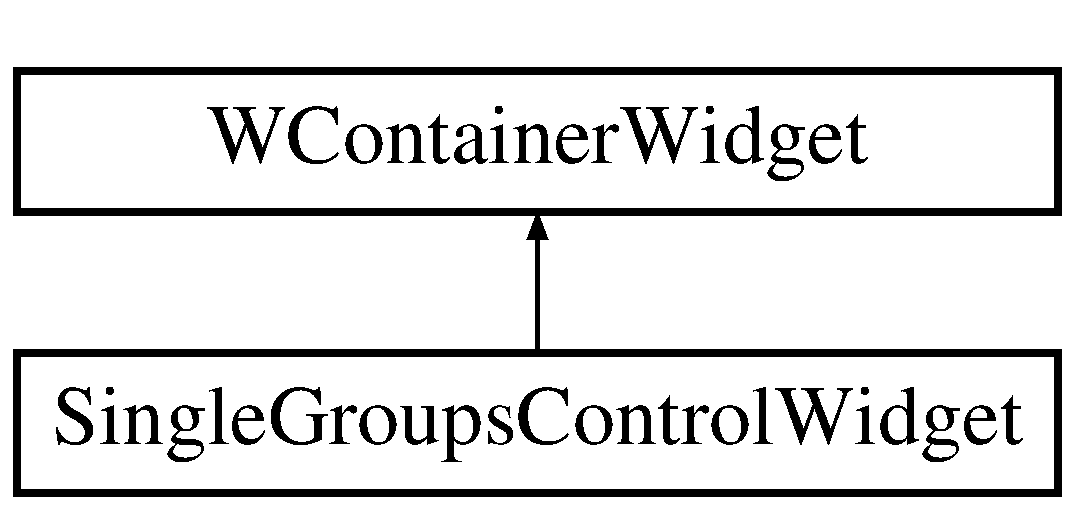
\includegraphics[height=2.000000cm]{class_single_groups_control_widget}
\end{center}
\end{figure}
\subsection*{Public Member Functions}
\begin{DoxyCompactItemize}
\item 
\hyperlink{class_single_groups_control_widget_a49e2f9e4c74289cf0d3167283e14fded}{Single\+Groups\+Control\+Widget} (\hyperlink{class_session}{Session} $\ast$session, Wt\+::\+W\+Container\+Widget $\ast$parent=0)
\begin{DoxyCompactList}\small\item\em creates a \hyperlink{class_single_groups_control_widget}{Single\+Groups\+Control\+Widget} \end{DoxyCompactList}\item 
void \hyperlink{class_single_groups_control_widget_ab6eea77943da3ae94d43764d2a5a4aed}{update} ()
\begin{DoxyCompactList}\small\item\em loads \hyperlink{class_single_groups_control_widget}{Single\+Groups\+Control\+Widget} page \end{DoxyCompactList}\end{DoxyCompactItemize}
\subsection*{Private Member Functions}
\begin{DoxyCompactItemize}
\item 
Wt\+::\+Http\+::\+Client $\ast$ \hyperlink{class_single_groups_control_widget_a36a607a09994c4c2db5ec8e214d2d5bc}{connect} ()
\begin{DoxyCompactList}\small\item\em creates an H\+T\+TP client \end{DoxyCompactList}\item 
void \hyperlink{class_single_groups_control_widget_ae1b39e4fd180f949cc6161a5837b659f}{on} ()
\begin{DoxyCompactList}\small\item\em turns group\textquotesingle{}s lights on \end{DoxyCompactList}\item 
void \hyperlink{class_single_groups_control_widget_a80dc0058c8bf19461f74a2efc6e40bdf}{off} ()
\begin{DoxyCompactList}\small\item\em turns group\textquotesingle{}s lights off \end{DoxyCompactList}\item 
void \hyperlink{class_single_groups_control_widget_a5da8fa2f328e6484b3cc3940ff09dd77}{hue} ()
\begin{DoxyCompactList}\small\item\em changes group\textquotesingle{}s hue \end{DoxyCompactList}\item 
void \hyperlink{class_single_groups_control_widget_abb243f17f45cd2f2d86147764f660b3e}{bright} ()
\begin{DoxyCompactList}\small\item\em changes group\textquotesingle{}s brightness \end{DoxyCompactList}\item 
void \hyperlink{class_single_groups_control_widget_aa1a21d1a2f3eeb2f9f73bb59dfaa7371}{sat} ()
\begin{DoxyCompactList}\small\item\em changes group\textquotesingle{}s saturation \end{DoxyCompactList}\item 
void \hyperlink{class_single_groups_control_widget_af9f44ae5837c9588dc4242e7a1ad4d7a}{name} ()
\begin{DoxyCompactList}\small\item\em changes group\textquotesingle{}s name \end{DoxyCompactList}\item 
void \hyperlink{class_single_groups_control_widget_a7ac224c22be007e2e3d944a5d93a2778}{transition} ()
\begin{DoxyCompactList}\small\item\em changes group\textquotesingle{}s transition time \end{DoxyCompactList}\item 
void \hyperlink{class_single_groups_control_widget_a3d83beb8c90183e11332bba1a4eab77d}{add\+Lights} ()
\begin{DoxyCompactList}\small\item\em adds light to group \end{DoxyCompactList}\item 
void \hyperlink{class_single_groups_control_widget_ab0729c8bad3c8ba43a22ed1af23ac6e7}{remove\+Lights} ()
\begin{DoxyCompactList}\small\item\em removes light from group \end{DoxyCompactList}\item 
void \hyperlink{class_single_groups_control_widget_a558dac00b479b6640de62b4812802250}{party\+Mode} ()
\begin{DoxyCompactList}\small\item\em puts group on party mode for 10s (color looping). Must wait for party mode to finish. \end{DoxyCompactList}\item 
void \hyperlink{class_single_groups_control_widget_a6cb68bd462d888756deba16b4e524470}{sunset\+Mode} ()
\begin{DoxyCompactList}\small\item\em puts group on sunset mode (yellows) \end{DoxyCompactList}\item 
void \hyperlink{class_single_groups_control_widget_a98a8fc3336b6d6a0ab087936c74955cc}{fifty\+Mode} ()
\begin{DoxyCompactList}\small\item\em puts group on fifty mode (greys) \end{DoxyCompactList}\item 
void \hyperlink{class_single_groups_control_widget_ad378bb04e410f93fd50eddc38c47d6d9}{mustang\+Mode} ()
\begin{DoxyCompactList}\small\item\em puts group on mustang mode (purples) \end{DoxyCompactList}\item 
void \hyperlink{class_single_groups_control_widget_a88810651632c7525970a816bdaa47d09}{blood\+Mode} ()
\begin{DoxyCompactList}\small\item\em puts group on blood mode (reds) \end{DoxyCompactList}\item 
void \hyperlink{class_single_groups_control_widget_afa302c84232d4a1fb69ef4da6528f0ec}{ocean\+Mode} ()
\begin{DoxyCompactList}\small\item\em puts group on ocean mode (blues) \end{DoxyCompactList}\item 
void \hyperlink{class_single_groups_control_widget_a41395f061e8d93131b0e8c1b880eab59}{fire\+Mode} ()
\begin{DoxyCompactList}\small\item\em puts group on fire mode (oranges) \end{DoxyCompactList}\item 
void \hyperlink{class_single_groups_control_widget_a6d940daceffefb6e5d17def4c4b24acc}{forest\+Mode} ()
\begin{DoxyCompactList}\small\item\em puts group on forest mode (greens) \end{DoxyCompactList}\item 
void \hyperlink{class_single_groups_control_widget_a1bb02de2f9fcda2cf5ef37c95d341975}{delete\+Group} ()
\begin{DoxyCompactList}\small\item\em deletes a group \end{DoxyCompactList}\item 
void \hyperlink{class_single_groups_control_widget_a25051151a10f35c0e196ccb0fd52f7f8}{return\+Bridge} ()
\begin{DoxyCompactList}\small\item\em returns user to bridge page \end{DoxyCompactList}\item 
void \hyperlink{class_single_groups_control_widget_a4aff4c45ad69e3fc391f89f14ecc1ebb}{handle\+Http\+Response} (boost\+::system\+::error\+\_\+code err, const Wt\+::\+Http\+::\+Message \&response)
\begin{DoxyCompactList}\small\item\em handles response and displays group information \end{DoxyCompactList}\item 
void \hyperlink{class_single_groups_control_widget_a5049556fc39b63323ab534ba65e398e3}{handle\+Http\+Response\+Update} (boost\+::system\+::error\+\_\+code err, const Wt\+::\+Http\+::\+Message \&response)
\begin{DoxyCompactList}\small\item\em handles response reloads page \end{DoxyCompactList}\item 
void \hyperlink{class_single_groups_control_widget_a8f1e4dc31eb242ce4284a1bad9d2fbcb}{handle\+Http\+Response\+V\+O\+ID} (boost\+::system\+::error\+\_\+code err, const Wt\+::\+Http\+::\+Message \&response)
\begin{DoxyCompactList}\small\item\em handles response and does nothing \end{DoxyCompactList}\end{DoxyCompactItemize}
\subsection*{Static Private Member Functions}
\begin{DoxyCompactItemize}
\item 
static void \hyperlink{class_single_groups_control_widget_adba20587e7d7afd7e7ef5d95b242579e}{music} (Wt\+::\+W\+Sound $\ast$sound)
\begin{DoxyCompactList}\small\item\em plays party.\+wav for party mode \end{DoxyCompactList}\end{DoxyCompactItemize}
\subsection*{Private Attributes}
\begin{DoxyCompactItemize}
\item 
\hyperlink{class_session}{Session} $\ast$ \hyperlink{class_single_groups_control_widget_af179b3aceb389ea2b7eb196c0cf2575d}{session\+\_\+}
\item 
std\+::string \hyperlink{class_single_groups_control_widget_a541ddd57077700f7a99ffca17636a771}{ip} = \char`\"{}\char`\"{}
\item 
std\+::string \hyperlink{class_single_groups_control_widget_a8e485f9b17c2934de11f8991a7b38bf6}{user\+ID} = \char`\"{}\char`\"{}
\item 
std\+::string \hyperlink{class_single_groups_control_widget_a6ce38d1d258028fcbefa83436ef49b5f}{port} = \char`\"{}\char`\"{}
\item 
std\+::string \hyperlink{class_single_groups_control_widget_ace03ddb209483e37c7f760fdb73baba7}{group\+ID} = \char`\"{}\char`\"{}
\item 
std\+::string \hyperlink{class_single_groups_control_widget_a0d6cf0bbd169e65cd4de29aea4a2e1b9}{lights}
\item 
bool \hyperlink{class_single_groups_control_widget_ab428d0f6a6c39724b434fc80e39c6b18}{delete\+Confirm}
\item 
Wt\+::\+W\+Line\+Edit $\ast$ \hyperlink{class_single_groups_control_widget_ab0dfc6fa2c8b3d5d2feb1858a1c3a2ef}{name\+Edit\+\_\+}
\item 
Wt\+::\+W\+Text $\ast$ \hyperlink{class_single_groups_control_widget_a2b80c0e1b05f5c1086d89512342d206f}{group\+Info\+Edit\+\_\+}
\item 
Wt\+::\+W\+Text $\ast$ \hyperlink{class_single_groups_control_widget_a0c5cd5692fc7b4be63b7732988021888}{group\+Lights\+Edit\+\_\+}
\item 
Wt\+::\+W\+Slider $\ast$ \hyperlink{class_single_groups_control_widget_ad41ed79fdff6691c6266f1a582b9962e}{sat\+Scale\+Slider\+\_\+}
\item 
Wt\+::\+W\+Slider $\ast$ \hyperlink{class_single_groups_control_widget_a761ff567fbcdc336c2b13ca9b9202478}{bri\+Scale\+Slider\+\_\+}
\item 
Wt\+::\+W\+Slider $\ast$ \hyperlink{class_single_groups_control_widget_adeb7eef1ab64cc98651ece9186e4dd68}{hue\+Scale\+Slider\+\_\+}
\item 
Wt\+::\+W\+Slider $\ast$ \hyperlink{class_single_groups_control_widget_af1811831d7031863931a9baaa97207a0}{transition\+Scale\+Slider\+\_\+}
\item 
Wt\+::\+W\+Text $\ast$ \hyperlink{class_single_groups_control_widget_a02fc84979ad2e0424a78ea3961c06a7d}{change\+\_\+}
\item 
Wt\+::\+W\+Combo\+Box $\ast$ \hyperlink{class_single_groups_control_widget_abd57b2068dc41172791d826f54dea64d}{add\+Choices\+\_\+}
\item 
Wt\+::\+W\+Combo\+Box $\ast$ \hyperlink{class_single_groups_control_widget_ad4558a087cef943d29674ec5ffd66381}{remove\+Choices\+\_\+}
\end{DoxyCompactItemize}


\subsection{Constructor \& Destructor Documentation}
\mbox{\Hypertarget{class_single_groups_control_widget_a49e2f9e4c74289cf0d3167283e14fded}\label{class_single_groups_control_widget_a49e2f9e4c74289cf0d3167283e14fded}} 
\index{Single\+Groups\+Control\+Widget@{Single\+Groups\+Control\+Widget}!Single\+Groups\+Control\+Widget@{Single\+Groups\+Control\+Widget}}
\index{Single\+Groups\+Control\+Widget@{Single\+Groups\+Control\+Widget}!Single\+Groups\+Control\+Widget@{Single\+Groups\+Control\+Widget}}
\subsubsection{\texorpdfstring{Single\+Groups\+Control\+Widget()}{SingleGroupsControlWidget()}}
{\footnotesize\ttfamily Single\+Groups\+Control\+Widget\+::\+Single\+Groups\+Control\+Widget (\begin{DoxyParamCaption}\item[{\hyperlink{class_session}{Session} $\ast$}]{session,  }\item[{Wt\+::\+W\+Container\+Widget $\ast$}]{parent = {\ttfamily 0} }\end{DoxyParamCaption})}



creates a \hyperlink{class_single_groups_control_widget}{Single\+Groups\+Control\+Widget} 


\begin{DoxyParams}{Parameters}
{\em session} & the database session \\
\hline
{\em parent} & the parent Widget Container \\
\hline
\end{DoxyParams}
\begin{DoxyReturn}{Returns}
\hyperlink{class_single_groups_control_widget}{Single\+Groups\+Control\+Widget} 
\end{DoxyReturn}


\subsection{Member Function Documentation}
\mbox{\Hypertarget{class_single_groups_control_widget_a3d83beb8c90183e11332bba1a4eab77d}\label{class_single_groups_control_widget_a3d83beb8c90183e11332bba1a4eab77d}} 
\index{Single\+Groups\+Control\+Widget@{Single\+Groups\+Control\+Widget}!add\+Lights@{add\+Lights}}
\index{add\+Lights@{add\+Lights}!Single\+Groups\+Control\+Widget@{Single\+Groups\+Control\+Widget}}
\subsubsection{\texorpdfstring{add\+Lights()}{addLights()}}
{\footnotesize\ttfamily void Single\+Groups\+Control\+Widget\+::add\+Lights (\begin{DoxyParamCaption}{ }\end{DoxyParamCaption})\hspace{0.3cm}{\ttfamily [private]}}



adds light to group 

\begin{DoxyReturn}{Returns}
Void 
\end{DoxyReturn}
\mbox{\Hypertarget{class_single_groups_control_widget_a88810651632c7525970a816bdaa47d09}\label{class_single_groups_control_widget_a88810651632c7525970a816bdaa47d09}} 
\index{Single\+Groups\+Control\+Widget@{Single\+Groups\+Control\+Widget}!blood\+Mode@{blood\+Mode}}
\index{blood\+Mode@{blood\+Mode}!Single\+Groups\+Control\+Widget@{Single\+Groups\+Control\+Widget}}
\subsubsection{\texorpdfstring{blood\+Mode()}{bloodMode()}}
{\footnotesize\ttfamily void Single\+Groups\+Control\+Widget\+::blood\+Mode (\begin{DoxyParamCaption}{ }\end{DoxyParamCaption})\hspace{0.3cm}{\ttfamily [private]}}



puts group on blood mode (reds) 

\begin{DoxyReturn}{Returns}
Void 
\end{DoxyReturn}
\mbox{\Hypertarget{class_single_groups_control_widget_abb243f17f45cd2f2d86147764f660b3e}\label{class_single_groups_control_widget_abb243f17f45cd2f2d86147764f660b3e}} 
\index{Single\+Groups\+Control\+Widget@{Single\+Groups\+Control\+Widget}!bright@{bright}}
\index{bright@{bright}!Single\+Groups\+Control\+Widget@{Single\+Groups\+Control\+Widget}}
\subsubsection{\texorpdfstring{bright()}{bright()}}
{\footnotesize\ttfamily void Single\+Groups\+Control\+Widget\+::bright (\begin{DoxyParamCaption}{ }\end{DoxyParamCaption})\hspace{0.3cm}{\ttfamily [private]}}



changes group\textquotesingle{}s brightness 

\begin{DoxyReturn}{Returns}
Void 
\end{DoxyReturn}
\mbox{\Hypertarget{class_single_groups_control_widget_a36a607a09994c4c2db5ec8e214d2d5bc}\label{class_single_groups_control_widget_a36a607a09994c4c2db5ec8e214d2d5bc}} 
\index{Single\+Groups\+Control\+Widget@{Single\+Groups\+Control\+Widget}!connect@{connect}}
\index{connect@{connect}!Single\+Groups\+Control\+Widget@{Single\+Groups\+Control\+Widget}}
\subsubsection{\texorpdfstring{connect()}{connect()}}
{\footnotesize\ttfamily Http\+::\+Client $\ast$ Single\+Groups\+Control\+Widget\+::connect (\begin{DoxyParamCaption}{ }\end{DoxyParamCaption})\hspace{0.3cm}{\ttfamily [private]}}



creates an H\+T\+TP client 

\begin{DoxyReturn}{Returns}
Http\+::\+Client 
\end{DoxyReturn}
\mbox{\Hypertarget{class_single_groups_control_widget_a1bb02de2f9fcda2cf5ef37c95d341975}\label{class_single_groups_control_widget_a1bb02de2f9fcda2cf5ef37c95d341975}} 
\index{Single\+Groups\+Control\+Widget@{Single\+Groups\+Control\+Widget}!delete\+Group@{delete\+Group}}
\index{delete\+Group@{delete\+Group}!Single\+Groups\+Control\+Widget@{Single\+Groups\+Control\+Widget}}
\subsubsection{\texorpdfstring{delete\+Group()}{deleteGroup()}}
{\footnotesize\ttfamily void Single\+Groups\+Control\+Widget\+::delete\+Group (\begin{DoxyParamCaption}{ }\end{DoxyParamCaption})\hspace{0.3cm}{\ttfamily [private]}}



deletes a group 

\begin{DoxyReturn}{Returns}
Void 
\end{DoxyReturn}
\mbox{\Hypertarget{class_single_groups_control_widget_a98a8fc3336b6d6a0ab087936c74955cc}\label{class_single_groups_control_widget_a98a8fc3336b6d6a0ab087936c74955cc}} 
\index{Single\+Groups\+Control\+Widget@{Single\+Groups\+Control\+Widget}!fifty\+Mode@{fifty\+Mode}}
\index{fifty\+Mode@{fifty\+Mode}!Single\+Groups\+Control\+Widget@{Single\+Groups\+Control\+Widget}}
\subsubsection{\texorpdfstring{fifty\+Mode()}{fiftyMode()}}
{\footnotesize\ttfamily void Single\+Groups\+Control\+Widget\+::fifty\+Mode (\begin{DoxyParamCaption}{ }\end{DoxyParamCaption})\hspace{0.3cm}{\ttfamily [private]}}



puts group on fifty mode (greys) 

\begin{DoxyReturn}{Returns}
Void 
\end{DoxyReturn}
\mbox{\Hypertarget{class_single_groups_control_widget_a41395f061e8d93131b0e8c1b880eab59}\label{class_single_groups_control_widget_a41395f061e8d93131b0e8c1b880eab59}} 
\index{Single\+Groups\+Control\+Widget@{Single\+Groups\+Control\+Widget}!fire\+Mode@{fire\+Mode}}
\index{fire\+Mode@{fire\+Mode}!Single\+Groups\+Control\+Widget@{Single\+Groups\+Control\+Widget}}
\subsubsection{\texorpdfstring{fire\+Mode()}{fireMode()}}
{\footnotesize\ttfamily void Single\+Groups\+Control\+Widget\+::fire\+Mode (\begin{DoxyParamCaption}{ }\end{DoxyParamCaption})\hspace{0.3cm}{\ttfamily [private]}}



puts group on fire mode (oranges) 

\begin{DoxyReturn}{Returns}
Void 
\end{DoxyReturn}
\mbox{\Hypertarget{class_single_groups_control_widget_a6d940daceffefb6e5d17def4c4b24acc}\label{class_single_groups_control_widget_a6d940daceffefb6e5d17def4c4b24acc}} 
\index{Single\+Groups\+Control\+Widget@{Single\+Groups\+Control\+Widget}!forest\+Mode@{forest\+Mode}}
\index{forest\+Mode@{forest\+Mode}!Single\+Groups\+Control\+Widget@{Single\+Groups\+Control\+Widget}}
\subsubsection{\texorpdfstring{forest\+Mode()}{forestMode()}}
{\footnotesize\ttfamily void Single\+Groups\+Control\+Widget\+::forest\+Mode (\begin{DoxyParamCaption}{ }\end{DoxyParamCaption})\hspace{0.3cm}{\ttfamily [private]}}



puts group on forest mode (greens) 

\begin{DoxyReturn}{Returns}
Void 
\end{DoxyReturn}
\mbox{\Hypertarget{class_single_groups_control_widget_a4aff4c45ad69e3fc391f89f14ecc1ebb}\label{class_single_groups_control_widget_a4aff4c45ad69e3fc391f89f14ecc1ebb}} 
\index{Single\+Groups\+Control\+Widget@{Single\+Groups\+Control\+Widget}!handle\+Http\+Response@{handle\+Http\+Response}}
\index{handle\+Http\+Response@{handle\+Http\+Response}!Single\+Groups\+Control\+Widget@{Single\+Groups\+Control\+Widget}}
\subsubsection{\texorpdfstring{handle\+Http\+Response()}{handleHttpResponse()}}
{\footnotesize\ttfamily void Single\+Groups\+Control\+Widget\+::handle\+Http\+Response (\begin{DoxyParamCaption}\item[{boost\+::system\+::error\+\_\+code}]{err,  }\item[{const Wt\+::\+Http\+::\+Message \&}]{response }\end{DoxyParamCaption})\hspace{0.3cm}{\ttfamily [private]}}



handles response and displays group information 


\begin{DoxyParams}{Parameters}
{\em err} & the response\textquotesingle{}s error code \\
\hline
{\em response} & the response \\
\hline
\end{DoxyParams}
\begin{DoxyReturn}{Returns}
Void 
\end{DoxyReturn}
\mbox{\Hypertarget{class_single_groups_control_widget_a5049556fc39b63323ab534ba65e398e3}\label{class_single_groups_control_widget_a5049556fc39b63323ab534ba65e398e3}} 
\index{Single\+Groups\+Control\+Widget@{Single\+Groups\+Control\+Widget}!handle\+Http\+Response\+Update@{handle\+Http\+Response\+Update}}
\index{handle\+Http\+Response\+Update@{handle\+Http\+Response\+Update}!Single\+Groups\+Control\+Widget@{Single\+Groups\+Control\+Widget}}
\subsubsection{\texorpdfstring{handle\+Http\+Response\+Update()}{handleHttpResponseUpdate()}}
{\footnotesize\ttfamily void Single\+Groups\+Control\+Widget\+::handle\+Http\+Response\+Update (\begin{DoxyParamCaption}\item[{boost\+::system\+::error\+\_\+code}]{err,  }\item[{const Wt\+::\+Http\+::\+Message \&}]{response }\end{DoxyParamCaption})\hspace{0.3cm}{\ttfamily [private]}}



handles response reloads page 


\begin{DoxyParams}{Parameters}
{\em err} & the response\textquotesingle{}s error code \\
\hline
{\em response} & the response \\
\hline
\end{DoxyParams}
\begin{DoxyReturn}{Returns}
Void 
\end{DoxyReturn}
\mbox{\Hypertarget{class_single_groups_control_widget_a8f1e4dc31eb242ce4284a1bad9d2fbcb}\label{class_single_groups_control_widget_a8f1e4dc31eb242ce4284a1bad9d2fbcb}} 
\index{Single\+Groups\+Control\+Widget@{Single\+Groups\+Control\+Widget}!handle\+Http\+Response\+V\+O\+ID@{handle\+Http\+Response\+V\+O\+ID}}
\index{handle\+Http\+Response\+V\+O\+ID@{handle\+Http\+Response\+V\+O\+ID}!Single\+Groups\+Control\+Widget@{Single\+Groups\+Control\+Widget}}
\subsubsection{\texorpdfstring{handle\+Http\+Response\+V\+O\+I\+D()}{handleHttpResponseVOID()}}
{\footnotesize\ttfamily void Single\+Groups\+Control\+Widget\+::handle\+Http\+Response\+V\+O\+ID (\begin{DoxyParamCaption}\item[{boost\+::system\+::error\+\_\+code}]{err,  }\item[{const Wt\+::\+Http\+::\+Message \&}]{response }\end{DoxyParamCaption})\hspace{0.3cm}{\ttfamily [private]}}



handles response and does nothing 


\begin{DoxyParams}{Parameters}
{\em err} & the response\textquotesingle{}s error code \\
\hline
{\em response} & the response \\
\hline
\end{DoxyParams}
\begin{DoxyReturn}{Returns}
Void 
\end{DoxyReturn}
\mbox{\Hypertarget{class_single_groups_control_widget_a5da8fa2f328e6484b3cc3940ff09dd77}\label{class_single_groups_control_widget_a5da8fa2f328e6484b3cc3940ff09dd77}} 
\index{Single\+Groups\+Control\+Widget@{Single\+Groups\+Control\+Widget}!hue@{hue}}
\index{hue@{hue}!Single\+Groups\+Control\+Widget@{Single\+Groups\+Control\+Widget}}
\subsubsection{\texorpdfstring{hue()}{hue()}}
{\footnotesize\ttfamily void Single\+Groups\+Control\+Widget\+::hue (\begin{DoxyParamCaption}{ }\end{DoxyParamCaption})\hspace{0.3cm}{\ttfamily [private]}}



changes group\textquotesingle{}s hue 

\begin{DoxyReturn}{Returns}
Void 
\end{DoxyReturn}
\mbox{\Hypertarget{class_single_groups_control_widget_adba20587e7d7afd7e7ef5d95b242579e}\label{class_single_groups_control_widget_adba20587e7d7afd7e7ef5d95b242579e}} 
\index{Single\+Groups\+Control\+Widget@{Single\+Groups\+Control\+Widget}!music@{music}}
\index{music@{music}!Single\+Groups\+Control\+Widget@{Single\+Groups\+Control\+Widget}}
\subsubsection{\texorpdfstring{music()}{music()}}
{\footnotesize\ttfamily static void Single\+Groups\+Control\+Widget\+::music (\begin{DoxyParamCaption}\item[{Wt\+::\+W\+Sound $\ast$}]{sound }\end{DoxyParamCaption})\hspace{0.3cm}{\ttfamily [static]}, {\ttfamily [private]}}



plays party.\+wav for party mode 


\begin{DoxyParams}{Parameters}
{\em sound} & audio file \\
\hline
\end{DoxyParams}
\begin{DoxyReturn}{Returns}
Void 
\end{DoxyReturn}
\mbox{\Hypertarget{class_single_groups_control_widget_ad378bb04e410f93fd50eddc38c47d6d9}\label{class_single_groups_control_widget_ad378bb04e410f93fd50eddc38c47d6d9}} 
\index{Single\+Groups\+Control\+Widget@{Single\+Groups\+Control\+Widget}!mustang\+Mode@{mustang\+Mode}}
\index{mustang\+Mode@{mustang\+Mode}!Single\+Groups\+Control\+Widget@{Single\+Groups\+Control\+Widget}}
\subsubsection{\texorpdfstring{mustang\+Mode()}{mustangMode()}}
{\footnotesize\ttfamily void Single\+Groups\+Control\+Widget\+::mustang\+Mode (\begin{DoxyParamCaption}{ }\end{DoxyParamCaption})\hspace{0.3cm}{\ttfamily [private]}}



puts group on mustang mode (purples) 

\begin{DoxyReturn}{Returns}
Void 
\end{DoxyReturn}
\mbox{\Hypertarget{class_single_groups_control_widget_af9f44ae5837c9588dc4242e7a1ad4d7a}\label{class_single_groups_control_widget_af9f44ae5837c9588dc4242e7a1ad4d7a}} 
\index{Single\+Groups\+Control\+Widget@{Single\+Groups\+Control\+Widget}!name@{name}}
\index{name@{name}!Single\+Groups\+Control\+Widget@{Single\+Groups\+Control\+Widget}}
\subsubsection{\texorpdfstring{name()}{name()}}
{\footnotesize\ttfamily void Single\+Groups\+Control\+Widget\+::name (\begin{DoxyParamCaption}{ }\end{DoxyParamCaption})\hspace{0.3cm}{\ttfamily [private]}}



changes group\textquotesingle{}s name 

\begin{DoxyReturn}{Returns}
Void 
\end{DoxyReturn}
\mbox{\Hypertarget{class_single_groups_control_widget_afa302c84232d4a1fb69ef4da6528f0ec}\label{class_single_groups_control_widget_afa302c84232d4a1fb69ef4da6528f0ec}} 
\index{Single\+Groups\+Control\+Widget@{Single\+Groups\+Control\+Widget}!ocean\+Mode@{ocean\+Mode}}
\index{ocean\+Mode@{ocean\+Mode}!Single\+Groups\+Control\+Widget@{Single\+Groups\+Control\+Widget}}
\subsubsection{\texorpdfstring{ocean\+Mode()}{oceanMode()}}
{\footnotesize\ttfamily void Single\+Groups\+Control\+Widget\+::ocean\+Mode (\begin{DoxyParamCaption}{ }\end{DoxyParamCaption})\hspace{0.3cm}{\ttfamily [private]}}



puts group on ocean mode (blues) 

\begin{DoxyReturn}{Returns}
Void 
\end{DoxyReturn}
\mbox{\Hypertarget{class_single_groups_control_widget_a80dc0058c8bf19461f74a2efc6e40bdf}\label{class_single_groups_control_widget_a80dc0058c8bf19461f74a2efc6e40bdf}} 
\index{Single\+Groups\+Control\+Widget@{Single\+Groups\+Control\+Widget}!off@{off}}
\index{off@{off}!Single\+Groups\+Control\+Widget@{Single\+Groups\+Control\+Widget}}
\subsubsection{\texorpdfstring{off()}{off()}}
{\footnotesize\ttfamily void Single\+Groups\+Control\+Widget\+::off (\begin{DoxyParamCaption}{ }\end{DoxyParamCaption})\hspace{0.3cm}{\ttfamily [private]}}



turns group\textquotesingle{}s lights off 

\begin{DoxyReturn}{Returns}
Void 
\end{DoxyReturn}
\mbox{\Hypertarget{class_single_groups_control_widget_ae1b39e4fd180f949cc6161a5837b659f}\label{class_single_groups_control_widget_ae1b39e4fd180f949cc6161a5837b659f}} 
\index{Single\+Groups\+Control\+Widget@{Single\+Groups\+Control\+Widget}!on@{on}}
\index{on@{on}!Single\+Groups\+Control\+Widget@{Single\+Groups\+Control\+Widget}}
\subsubsection{\texorpdfstring{on()}{on()}}
{\footnotesize\ttfamily void Single\+Groups\+Control\+Widget\+::on (\begin{DoxyParamCaption}{ }\end{DoxyParamCaption})\hspace{0.3cm}{\ttfamily [private]}}



turns group\textquotesingle{}s lights on 

\begin{DoxyReturn}{Returns}
Void 
\end{DoxyReturn}
\mbox{\Hypertarget{class_single_groups_control_widget_a558dac00b479b6640de62b4812802250}\label{class_single_groups_control_widget_a558dac00b479b6640de62b4812802250}} 
\index{Single\+Groups\+Control\+Widget@{Single\+Groups\+Control\+Widget}!party\+Mode@{party\+Mode}}
\index{party\+Mode@{party\+Mode}!Single\+Groups\+Control\+Widget@{Single\+Groups\+Control\+Widget}}
\subsubsection{\texorpdfstring{party\+Mode()}{partyMode()}}
{\footnotesize\ttfamily void Single\+Groups\+Control\+Widget\+::party\+Mode (\begin{DoxyParamCaption}{ }\end{DoxyParamCaption})\hspace{0.3cm}{\ttfamily [private]}}



puts group on party mode for 10s (color looping). Must wait for party mode to finish. 

\begin{DoxyReturn}{Returns}
Void 
\end{DoxyReturn}
\mbox{\Hypertarget{class_single_groups_control_widget_ab0729c8bad3c8ba43a22ed1af23ac6e7}\label{class_single_groups_control_widget_ab0729c8bad3c8ba43a22ed1af23ac6e7}} 
\index{Single\+Groups\+Control\+Widget@{Single\+Groups\+Control\+Widget}!remove\+Lights@{remove\+Lights}}
\index{remove\+Lights@{remove\+Lights}!Single\+Groups\+Control\+Widget@{Single\+Groups\+Control\+Widget}}
\subsubsection{\texorpdfstring{remove\+Lights()}{removeLights()}}
{\footnotesize\ttfamily void Single\+Groups\+Control\+Widget\+::remove\+Lights (\begin{DoxyParamCaption}{ }\end{DoxyParamCaption})\hspace{0.3cm}{\ttfamily [private]}}



removes light from group 

\begin{DoxyReturn}{Returns}
Void 
\end{DoxyReturn}
\mbox{\Hypertarget{class_single_groups_control_widget_a25051151a10f35c0e196ccb0fd52f7f8}\label{class_single_groups_control_widget_a25051151a10f35c0e196ccb0fd52f7f8}} 
\index{Single\+Groups\+Control\+Widget@{Single\+Groups\+Control\+Widget}!return\+Bridge@{return\+Bridge}}
\index{return\+Bridge@{return\+Bridge}!Single\+Groups\+Control\+Widget@{Single\+Groups\+Control\+Widget}}
\subsubsection{\texorpdfstring{return\+Bridge()}{returnBridge()}}
{\footnotesize\ttfamily void Single\+Groups\+Control\+Widget\+::return\+Bridge (\begin{DoxyParamCaption}{ }\end{DoxyParamCaption})\hspace{0.3cm}{\ttfamily [private]}}



returns user to bridge page 

\begin{DoxyReturn}{Returns}
Void 
\end{DoxyReturn}
\mbox{\Hypertarget{class_single_groups_control_widget_aa1a21d1a2f3eeb2f9f73bb59dfaa7371}\label{class_single_groups_control_widget_aa1a21d1a2f3eeb2f9f73bb59dfaa7371}} 
\index{Single\+Groups\+Control\+Widget@{Single\+Groups\+Control\+Widget}!sat@{sat}}
\index{sat@{sat}!Single\+Groups\+Control\+Widget@{Single\+Groups\+Control\+Widget}}
\subsubsection{\texorpdfstring{sat()}{sat()}}
{\footnotesize\ttfamily void Single\+Groups\+Control\+Widget\+::sat (\begin{DoxyParamCaption}{ }\end{DoxyParamCaption})\hspace{0.3cm}{\ttfamily [private]}}



changes group\textquotesingle{}s saturation 

\begin{DoxyReturn}{Returns}
Void 
\end{DoxyReturn}
\mbox{\Hypertarget{class_single_groups_control_widget_a6cb68bd462d888756deba16b4e524470}\label{class_single_groups_control_widget_a6cb68bd462d888756deba16b4e524470}} 
\index{Single\+Groups\+Control\+Widget@{Single\+Groups\+Control\+Widget}!sunset\+Mode@{sunset\+Mode}}
\index{sunset\+Mode@{sunset\+Mode}!Single\+Groups\+Control\+Widget@{Single\+Groups\+Control\+Widget}}
\subsubsection{\texorpdfstring{sunset\+Mode()}{sunsetMode()}}
{\footnotesize\ttfamily void Single\+Groups\+Control\+Widget\+::sunset\+Mode (\begin{DoxyParamCaption}{ }\end{DoxyParamCaption})\hspace{0.3cm}{\ttfamily [private]}}



puts group on sunset mode (yellows) 

\begin{DoxyReturn}{Returns}
Void 
\end{DoxyReturn}
\mbox{\Hypertarget{class_single_groups_control_widget_a7ac224c22be007e2e3d944a5d93a2778}\label{class_single_groups_control_widget_a7ac224c22be007e2e3d944a5d93a2778}} 
\index{Single\+Groups\+Control\+Widget@{Single\+Groups\+Control\+Widget}!transition@{transition}}
\index{transition@{transition}!Single\+Groups\+Control\+Widget@{Single\+Groups\+Control\+Widget}}
\subsubsection{\texorpdfstring{transition()}{transition()}}
{\footnotesize\ttfamily void Single\+Groups\+Control\+Widget\+::transition (\begin{DoxyParamCaption}{ }\end{DoxyParamCaption})\hspace{0.3cm}{\ttfamily [private]}}



changes group\textquotesingle{}s transition time 

\begin{DoxyReturn}{Returns}
Void 
\end{DoxyReturn}
\mbox{\Hypertarget{class_single_groups_control_widget_ab6eea77943da3ae94d43764d2a5a4aed}\label{class_single_groups_control_widget_ab6eea77943da3ae94d43764d2a5a4aed}} 
\index{Single\+Groups\+Control\+Widget@{Single\+Groups\+Control\+Widget}!update@{update}}
\index{update@{update}!Single\+Groups\+Control\+Widget@{Single\+Groups\+Control\+Widget}}
\subsubsection{\texorpdfstring{update()}{update()}}
{\footnotesize\ttfamily void Single\+Groups\+Control\+Widget\+::update (\begin{DoxyParamCaption}{ }\end{DoxyParamCaption})}



loads \hyperlink{class_single_groups_control_widget}{Single\+Groups\+Control\+Widget} page 

\begin{DoxyReturn}{Returns}
Void 
\end{DoxyReturn}


\subsection{Member Data Documentation}
\mbox{\Hypertarget{class_single_groups_control_widget_abd57b2068dc41172791d826f54dea64d}\label{class_single_groups_control_widget_abd57b2068dc41172791d826f54dea64d}} 
\index{Single\+Groups\+Control\+Widget@{Single\+Groups\+Control\+Widget}!add\+Choices\+\_\+@{add\+Choices\+\_\+}}
\index{add\+Choices\+\_\+@{add\+Choices\+\_\+}!Single\+Groups\+Control\+Widget@{Single\+Groups\+Control\+Widget}}
\subsubsection{\texorpdfstring{add\+Choices\+\_\+}{addChoices\_}}
{\footnotesize\ttfamily Wt\+::\+W\+Combo\+Box$\ast$ Single\+Groups\+Control\+Widget\+::add\+Choices\+\_\+\hspace{0.3cm}{\ttfamily [private]}}

selected light to add to group \mbox{\Hypertarget{class_single_groups_control_widget_a761ff567fbcdc336c2b13ca9b9202478}\label{class_single_groups_control_widget_a761ff567fbcdc336c2b13ca9b9202478}} 
\index{Single\+Groups\+Control\+Widget@{Single\+Groups\+Control\+Widget}!bri\+Scale\+Slider\+\_\+@{bri\+Scale\+Slider\+\_\+}}
\index{bri\+Scale\+Slider\+\_\+@{bri\+Scale\+Slider\+\_\+}!Single\+Groups\+Control\+Widget@{Single\+Groups\+Control\+Widget}}
\subsubsection{\texorpdfstring{bri\+Scale\+Slider\+\_\+}{briScaleSlider\_}}
{\footnotesize\ttfamily Wt\+::\+W\+Slider$\ast$ Single\+Groups\+Control\+Widget\+::bri\+Scale\+Slider\+\_\+\hspace{0.3cm}{\ttfamily [private]}}

group\textquotesingle{}s brightness to change into \mbox{\Hypertarget{class_single_groups_control_widget_a02fc84979ad2e0424a78ea3961c06a7d}\label{class_single_groups_control_widget_a02fc84979ad2e0424a78ea3961c06a7d}} 
\index{Single\+Groups\+Control\+Widget@{Single\+Groups\+Control\+Widget}!change\+\_\+@{change\+\_\+}}
\index{change\+\_\+@{change\+\_\+}!Single\+Groups\+Control\+Widget@{Single\+Groups\+Control\+Widget}}
\subsubsection{\texorpdfstring{change\+\_\+}{change\_}}
{\footnotesize\ttfamily Wt\+::\+W\+Text$\ast$ Single\+Groups\+Control\+Widget\+::change\+\_\+\hspace{0.3cm}{\ttfamily [private]}}

status of a group change \mbox{\Hypertarget{class_single_groups_control_widget_ab428d0f6a6c39724b434fc80e39c6b18}\label{class_single_groups_control_widget_ab428d0f6a6c39724b434fc80e39c6b18}} 
\index{Single\+Groups\+Control\+Widget@{Single\+Groups\+Control\+Widget}!delete\+Confirm@{delete\+Confirm}}
\index{delete\+Confirm@{delete\+Confirm}!Single\+Groups\+Control\+Widget@{Single\+Groups\+Control\+Widget}}
\subsubsection{\texorpdfstring{delete\+Confirm}{deleteConfirm}}
{\footnotesize\ttfamily bool Single\+Groups\+Control\+Widget\+::delete\+Confirm\hspace{0.3cm}{\ttfamily [private]}}

confirmation of intent to delete group \mbox{\Hypertarget{class_single_groups_control_widget_ace03ddb209483e37c7f760fdb73baba7}\label{class_single_groups_control_widget_ace03ddb209483e37c7f760fdb73baba7}} 
\index{Single\+Groups\+Control\+Widget@{Single\+Groups\+Control\+Widget}!group\+ID@{group\+ID}}
\index{group\+ID@{group\+ID}!Single\+Groups\+Control\+Widget@{Single\+Groups\+Control\+Widget}}
\subsubsection{\texorpdfstring{group\+ID}{groupID}}
{\footnotesize\ttfamily std\+::string Single\+Groups\+Control\+Widget\+::group\+ID = \char`\"{}\char`\"{}\hspace{0.3cm}{\ttfamily [private]}}

group\textquotesingle{}s ID \mbox{\Hypertarget{class_single_groups_control_widget_a2b80c0e1b05f5c1086d89512342d206f}\label{class_single_groups_control_widget_a2b80c0e1b05f5c1086d89512342d206f}} 
\index{Single\+Groups\+Control\+Widget@{Single\+Groups\+Control\+Widget}!group\+Info\+Edit\+\_\+@{group\+Info\+Edit\+\_\+}}
\index{group\+Info\+Edit\+\_\+@{group\+Info\+Edit\+\_\+}!Single\+Groups\+Control\+Widget@{Single\+Groups\+Control\+Widget}}
\subsubsection{\texorpdfstring{group\+Info\+Edit\+\_\+}{groupInfoEdit\_}}
{\footnotesize\ttfamily Wt\+::\+W\+Text$\ast$ Single\+Groups\+Control\+Widget\+::group\+Info\+Edit\+\_\+\hspace{0.3cm}{\ttfamily [private]}}

group name display \mbox{\Hypertarget{class_single_groups_control_widget_a0c5cd5692fc7b4be63b7732988021888}\label{class_single_groups_control_widget_a0c5cd5692fc7b4be63b7732988021888}} 
\index{Single\+Groups\+Control\+Widget@{Single\+Groups\+Control\+Widget}!group\+Lights\+Edit\+\_\+@{group\+Lights\+Edit\+\_\+}}
\index{group\+Lights\+Edit\+\_\+@{group\+Lights\+Edit\+\_\+}!Single\+Groups\+Control\+Widget@{Single\+Groups\+Control\+Widget}}
\subsubsection{\texorpdfstring{group\+Lights\+Edit\+\_\+}{groupLightsEdit\_}}
{\footnotesize\ttfamily Wt\+::\+W\+Text$\ast$ Single\+Groups\+Control\+Widget\+::group\+Lights\+Edit\+\_\+\hspace{0.3cm}{\ttfamily [private]}}

group\textquotesingle{}s light display \mbox{\Hypertarget{class_single_groups_control_widget_adeb7eef1ab64cc98651ece9186e4dd68}\label{class_single_groups_control_widget_adeb7eef1ab64cc98651ece9186e4dd68}} 
\index{Single\+Groups\+Control\+Widget@{Single\+Groups\+Control\+Widget}!hue\+Scale\+Slider\+\_\+@{hue\+Scale\+Slider\+\_\+}}
\index{hue\+Scale\+Slider\+\_\+@{hue\+Scale\+Slider\+\_\+}!Single\+Groups\+Control\+Widget@{Single\+Groups\+Control\+Widget}}
\subsubsection{\texorpdfstring{hue\+Scale\+Slider\+\_\+}{hueScaleSlider\_}}
{\footnotesize\ttfamily Wt\+::\+W\+Slider$\ast$ Single\+Groups\+Control\+Widget\+::hue\+Scale\+Slider\+\_\+\hspace{0.3cm}{\ttfamily [private]}}

group\textquotesingle{}s hue to change into \mbox{\Hypertarget{class_single_groups_control_widget_a541ddd57077700f7a99ffca17636a771}\label{class_single_groups_control_widget_a541ddd57077700f7a99ffca17636a771}} 
\index{Single\+Groups\+Control\+Widget@{Single\+Groups\+Control\+Widget}!ip@{ip}}
\index{ip@{ip}!Single\+Groups\+Control\+Widget@{Single\+Groups\+Control\+Widget}}
\subsubsection{\texorpdfstring{ip}{ip}}
{\footnotesize\ttfamily std\+::string Single\+Groups\+Control\+Widget\+::ip = \char`\"{}\char`\"{}\hspace{0.3cm}{\ttfamily [private]}}

bridge\textquotesingle{}s IP address \mbox{\Hypertarget{class_single_groups_control_widget_a0d6cf0bbd169e65cd4de29aea4a2e1b9}\label{class_single_groups_control_widget_a0d6cf0bbd169e65cd4de29aea4a2e1b9}} 
\index{Single\+Groups\+Control\+Widget@{Single\+Groups\+Control\+Widget}!lights@{lights}}
\index{lights@{lights}!Single\+Groups\+Control\+Widget@{Single\+Groups\+Control\+Widget}}
\subsubsection{\texorpdfstring{lights}{lights}}
{\footnotesize\ttfamily std\+::string Single\+Groups\+Control\+Widget\+::lights\hspace{0.3cm}{\ttfamily [private]}}

group\textquotesingle{}s lights \mbox{\Hypertarget{class_single_groups_control_widget_ab0dfc6fa2c8b3d5d2feb1858a1c3a2ef}\label{class_single_groups_control_widget_ab0dfc6fa2c8b3d5d2feb1858a1c3a2ef}} 
\index{Single\+Groups\+Control\+Widget@{Single\+Groups\+Control\+Widget}!name\+Edit\+\_\+@{name\+Edit\+\_\+}}
\index{name\+Edit\+\_\+@{name\+Edit\+\_\+}!Single\+Groups\+Control\+Widget@{Single\+Groups\+Control\+Widget}}
\subsubsection{\texorpdfstring{name\+Edit\+\_\+}{nameEdit\_}}
{\footnotesize\ttfamily Wt\+::\+W\+Line\+Edit$\ast$ Single\+Groups\+Control\+Widget\+::name\+Edit\+\_\+\hspace{0.3cm}{\ttfamily [private]}}

groups\textquotesingle{} name to be changed \mbox{\Hypertarget{class_single_groups_control_widget_a6ce38d1d258028fcbefa83436ef49b5f}\label{class_single_groups_control_widget_a6ce38d1d258028fcbefa83436ef49b5f}} 
\index{Single\+Groups\+Control\+Widget@{Single\+Groups\+Control\+Widget}!port@{port}}
\index{port@{port}!Single\+Groups\+Control\+Widget@{Single\+Groups\+Control\+Widget}}
\subsubsection{\texorpdfstring{port}{port}}
{\footnotesize\ttfamily std\+::string Single\+Groups\+Control\+Widget\+::port = \char`\"{}\char`\"{}\hspace{0.3cm}{\ttfamily [private]}}

bridge\textquotesingle{}s port number \mbox{\Hypertarget{class_single_groups_control_widget_ad4558a087cef943d29674ec5ffd66381}\label{class_single_groups_control_widget_ad4558a087cef943d29674ec5ffd66381}} 
\index{Single\+Groups\+Control\+Widget@{Single\+Groups\+Control\+Widget}!remove\+Choices\+\_\+@{remove\+Choices\+\_\+}}
\index{remove\+Choices\+\_\+@{remove\+Choices\+\_\+}!Single\+Groups\+Control\+Widget@{Single\+Groups\+Control\+Widget}}
\subsubsection{\texorpdfstring{remove\+Choices\+\_\+}{removeChoices\_}}
{\footnotesize\ttfamily Wt\+::\+W\+Combo\+Box$\ast$ Single\+Groups\+Control\+Widget\+::remove\+Choices\+\_\+\hspace{0.3cm}{\ttfamily [private]}}

selected light to remove from group \mbox{\Hypertarget{class_single_groups_control_widget_ad41ed79fdff6691c6266f1a582b9962e}\label{class_single_groups_control_widget_ad41ed79fdff6691c6266f1a582b9962e}} 
\index{Single\+Groups\+Control\+Widget@{Single\+Groups\+Control\+Widget}!sat\+Scale\+Slider\+\_\+@{sat\+Scale\+Slider\+\_\+}}
\index{sat\+Scale\+Slider\+\_\+@{sat\+Scale\+Slider\+\_\+}!Single\+Groups\+Control\+Widget@{Single\+Groups\+Control\+Widget}}
\subsubsection{\texorpdfstring{sat\+Scale\+Slider\+\_\+}{satScaleSlider\_}}
{\footnotesize\ttfamily Wt\+::\+W\+Slider$\ast$ Single\+Groups\+Control\+Widget\+::sat\+Scale\+Slider\+\_\+\hspace{0.3cm}{\ttfamily [private]}}

group\textquotesingle{}s saturation to change into \mbox{\Hypertarget{class_single_groups_control_widget_af179b3aceb389ea2b7eb196c0cf2575d}\label{class_single_groups_control_widget_af179b3aceb389ea2b7eb196c0cf2575d}} 
\index{Single\+Groups\+Control\+Widget@{Single\+Groups\+Control\+Widget}!session\+\_\+@{session\+\_\+}}
\index{session\+\_\+@{session\+\_\+}!Single\+Groups\+Control\+Widget@{Single\+Groups\+Control\+Widget}}
\subsubsection{\texorpdfstring{session\+\_\+}{session\_}}
{\footnotesize\ttfamily \hyperlink{class_session}{Session}$\ast$ Single\+Groups\+Control\+Widget\+::session\+\_\+\hspace{0.3cm}{\ttfamily [private]}}

keeps track of group status \mbox{\Hypertarget{class_single_groups_control_widget_af1811831d7031863931a9baaa97207a0}\label{class_single_groups_control_widget_af1811831d7031863931a9baaa97207a0}} 
\index{Single\+Groups\+Control\+Widget@{Single\+Groups\+Control\+Widget}!transition\+Scale\+Slider\+\_\+@{transition\+Scale\+Slider\+\_\+}}
\index{transition\+Scale\+Slider\+\_\+@{transition\+Scale\+Slider\+\_\+}!Single\+Groups\+Control\+Widget@{Single\+Groups\+Control\+Widget}}
\subsubsection{\texorpdfstring{transition\+Scale\+Slider\+\_\+}{transitionScaleSlider\_}}
{\footnotesize\ttfamily Wt\+::\+W\+Slider$\ast$ Single\+Groups\+Control\+Widget\+::transition\+Scale\+Slider\+\_\+\hspace{0.3cm}{\ttfamily [private]}}

group\textquotesingle{}s transition time to change into \mbox{\Hypertarget{class_single_groups_control_widget_a8e485f9b17c2934de11f8991a7b38bf6}\label{class_single_groups_control_widget_a8e485f9b17c2934de11f8991a7b38bf6}} 
\index{Single\+Groups\+Control\+Widget@{Single\+Groups\+Control\+Widget}!user\+ID@{user\+ID}}
\index{user\+ID@{user\+ID}!Single\+Groups\+Control\+Widget@{Single\+Groups\+Control\+Widget}}
\subsubsection{\texorpdfstring{user\+ID}{userID}}
{\footnotesize\ttfamily std\+::string Single\+Groups\+Control\+Widget\+::user\+ID = \char`\"{}\char`\"{}\hspace{0.3cm}{\ttfamily [private]}}

user\textquotesingle{}s bridge ID 

The documentation for this class was generated from the following files\+:\begin{DoxyCompactItemize}
\item 
\hyperlink{_single_groups_control_8h}{Single\+Groups\+Control.\+h}\item 
\hyperlink{_single_groups_control_8_c}{Single\+Groups\+Control.\+C}\end{DoxyCompactItemize}

\hypertarget{class_user}{}\section{User Class Reference}
\label{class_user}\index{User@{User}}


{\ttfamily \#include $<$User.\+h$>$}

\subsection*{Public Member Functions}
\begin{DoxyCompactItemize}
\item 
\hyperlink{class_user_a4a0137053e591fbb79d9057dd7d2283d}{User} ()
\item 
{\footnotesize template$<$class Action $>$ }\\void \hyperlink{class_user_a626b516f8e54e0b98c4b20c488de01b8}{persist} (Action \&a)
\end{DoxyCompactItemize}
\subsection*{Public Attributes}
\begin{DoxyCompactItemize}
\item 
std\+::string \hyperlink{class_user_a085d8d69282b6298964eab8351584536}{name}
\item 
std\+::string \hyperlink{class_user_aa845739b31aaf9d2e7bdedf829447191}{first\+Name}
\item 
std\+::string \hyperlink{class_user_a10abe0efedb0a600a7be16593a448b12}{last\+Name}
\item 
std\+::string \hyperlink{class_user_ac35b7c63228119cb91acdbd7ed32b8cb}{email}
\item 
std\+::string \hyperlink{class_user_aab2b993a0e6512bed3f637338f48d9ac}{bridge\+User\+ID}
\item 
Wt\+::\+Dbo\+::collection$<$ Wt\+::\+Dbo\+::ptr$<$ \hyperlink{class_bridge}{Bridge} $>$ $>$ \hyperlink{class_user_a19170eac8428770570d1e0b826562131}{bridges}
\item 
Wt\+::\+Dbo\+::collection$<$ Wt\+::\+Dbo\+::ptr$<$ \hyperlink{_user_8h_a3c0a51912624b328e151e753cb0d1dd3}{Auth\+Info} $>$ $>$ \hyperlink{class_user_ae3f58fe31642f514288705f4081031b6}{auth\+Infos}
\end{DoxyCompactItemize}


\subsection{Constructor \& Destructor Documentation}
\mbox{\Hypertarget{class_user_a4a0137053e591fbb79d9057dd7d2283d}\label{class_user_a4a0137053e591fbb79d9057dd7d2283d}} 
\index{User@{User}!User@{User}}
\index{User@{User}!User@{User}}
\subsubsection{\texorpdfstring{User()}{User()}}
{\footnotesize\ttfamily User\+::\+User (\begin{DoxyParamCaption}{ }\end{DoxyParamCaption})}



\subsection{Member Function Documentation}
\mbox{\Hypertarget{class_user_a626b516f8e54e0b98c4b20c488de01b8}\label{class_user_a626b516f8e54e0b98c4b20c488de01b8}} 
\index{User@{User}!persist@{persist}}
\index{persist@{persist}!User@{User}}
\subsubsection{\texorpdfstring{persist()}{persist()}}
{\footnotesize\ttfamily template$<$class Action $>$ \\
void User\+::persist (\begin{DoxyParamCaption}\item[{Action \&}]{a }\end{DoxyParamCaption})\hspace{0.3cm}{\ttfamily [inline]}}



\subsection{Member Data Documentation}
\mbox{\Hypertarget{class_user_ae3f58fe31642f514288705f4081031b6}\label{class_user_ae3f58fe31642f514288705f4081031b6}} 
\index{User@{User}!auth\+Infos@{auth\+Infos}}
\index{auth\+Infos@{auth\+Infos}!User@{User}}
\subsubsection{\texorpdfstring{auth\+Infos}{authInfos}}
{\footnotesize\ttfamily Wt\+::\+Dbo\+::collection$<$ Wt\+::\+Dbo\+::ptr$<$\hyperlink{_user_8h_a3c0a51912624b328e151e753cb0d1dd3}{Auth\+Info}$>$ $>$ User\+::auth\+Infos}

\mbox{\Hypertarget{class_user_a19170eac8428770570d1e0b826562131}\label{class_user_a19170eac8428770570d1e0b826562131}} 
\index{User@{User}!bridges@{bridges}}
\index{bridges@{bridges}!User@{User}}
\subsubsection{\texorpdfstring{bridges}{bridges}}
{\footnotesize\ttfamily Wt\+::\+Dbo\+::collection$<$Wt\+::\+Dbo\+::ptr$<$\hyperlink{class_bridge}{Bridge}$>$ $>$ User\+::bridges}

\mbox{\Hypertarget{class_user_aab2b993a0e6512bed3f637338f48d9ac}\label{class_user_aab2b993a0e6512bed3f637338f48d9ac}} 
\index{User@{User}!bridge\+User\+ID@{bridge\+User\+ID}}
\index{bridge\+User\+ID@{bridge\+User\+ID}!User@{User}}
\subsubsection{\texorpdfstring{bridge\+User\+ID}{bridgeUserID}}
{\footnotesize\ttfamily std\+::string User\+::bridge\+User\+ID}

\mbox{\Hypertarget{class_user_ac35b7c63228119cb91acdbd7ed32b8cb}\label{class_user_ac35b7c63228119cb91acdbd7ed32b8cb}} 
\index{User@{User}!email@{email}}
\index{email@{email}!User@{User}}
\subsubsection{\texorpdfstring{email}{email}}
{\footnotesize\ttfamily std\+::string User\+::email}

\mbox{\Hypertarget{class_user_aa845739b31aaf9d2e7bdedf829447191}\label{class_user_aa845739b31aaf9d2e7bdedf829447191}} 
\index{User@{User}!first\+Name@{first\+Name}}
\index{first\+Name@{first\+Name}!User@{User}}
\subsubsection{\texorpdfstring{first\+Name}{firstName}}
{\footnotesize\ttfamily std\+::string User\+::first\+Name}

\mbox{\Hypertarget{class_user_a10abe0efedb0a600a7be16593a448b12}\label{class_user_a10abe0efedb0a600a7be16593a448b12}} 
\index{User@{User}!last\+Name@{last\+Name}}
\index{last\+Name@{last\+Name}!User@{User}}
\subsubsection{\texorpdfstring{last\+Name}{lastName}}
{\footnotesize\ttfamily std\+::string User\+::last\+Name}

\mbox{\Hypertarget{class_user_a085d8d69282b6298964eab8351584536}\label{class_user_a085d8d69282b6298964eab8351584536}} 
\index{User@{User}!name@{name}}
\index{name@{name}!User@{User}}
\subsubsection{\texorpdfstring{name}{name}}
{\footnotesize\ttfamily std\+::string User\+::name}



The documentation for this class was generated from the following files\+:\begin{DoxyCompactItemize}
\item 
\hyperlink{_user_8h}{User.\+h}\item 
\hyperlink{_user_8_c}{User.\+C}\end{DoxyCompactItemize}

\hypertarget{class_user_details_model}{}\section{User\+Details\+Model Class Reference}
\label{class_user_details_model}\index{User\+Details\+Model@{User\+Details\+Model}}


{\ttfamily \#include $<$User\+Details\+Model.\+h$>$}

Inheritance diagram for User\+Details\+Model\+:\begin{figure}[H]
\begin{center}
\leavevmode
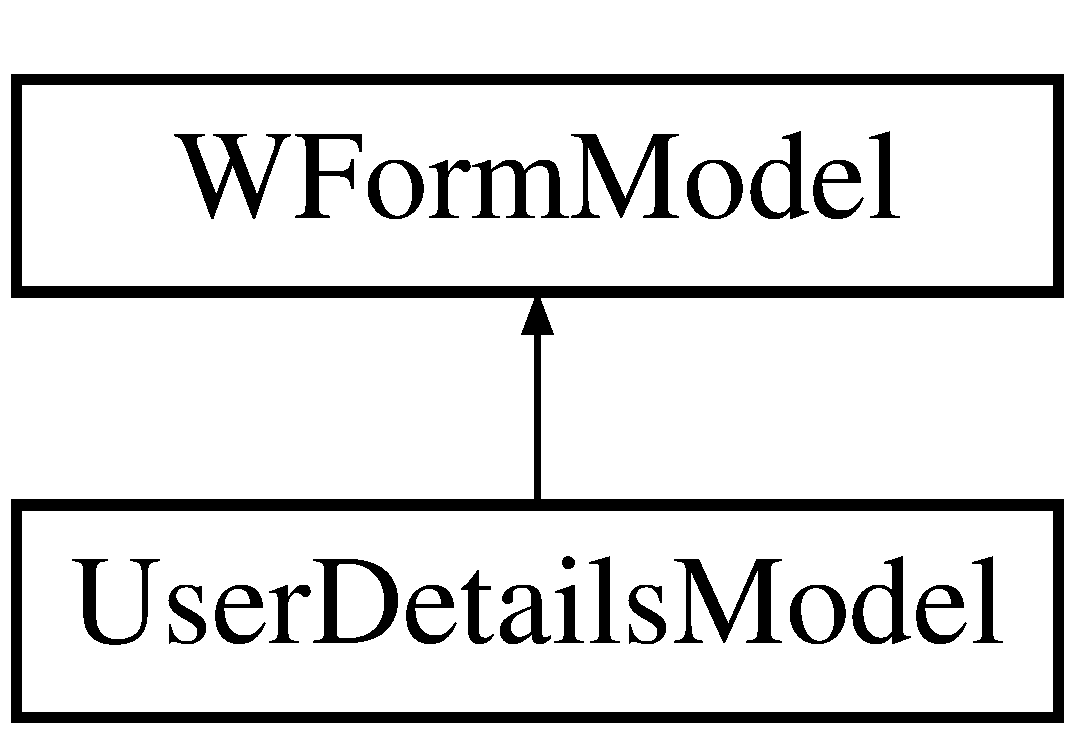
\includegraphics[height=2.000000cm]{class_user_details_model}
\end{center}
\end{figure}
\subsection*{Public Member Functions}
\begin{DoxyCompactItemize}
\item 
\hyperlink{class_user_details_model_aac16af78a18e4a99a6666d85914af5d5}{User\+Details\+Model} (\hyperlink{class_session}{Session} \&session, Wt\+::\+W\+Object $\ast$parent=0)
\item 
void \hyperlink{class_user_details_model_a0216d9fc37c8528a5fd49756529d4f57}{save} (const Wt\+::\+Auth\+::\+User \&user)
\end{DoxyCompactItemize}
\subsection*{Static Public Attributes}
\begin{DoxyCompactItemize}
\item 
static const Field \hyperlink{class_user_details_model_a5106e62fceceff6333718c1c88cee6cf}{First\+Name\+Field} = \char`\"{}first-\/\hyperlink{_bridge_control_8_c_a8ccf841cb59e451791bcb2e1ac4f1edc}{name}\char`\"{}
\item 
static const Field \hyperlink{class_user_details_model_a1d1e2d4300151876ed221b080860b004}{Last\+Name\+Field} = \char`\"{}last-\/\hyperlink{_bridge_control_8_c_a8ccf841cb59e451791bcb2e1ac4f1edc}{name}\char`\"{}
\end{DoxyCompactItemize}
\subsection*{Private Attributes}
\begin{DoxyCompactItemize}
\item 
\hyperlink{class_session}{Session} \& \hyperlink{class_user_details_model_a97ed29b3f1835399da3765b50f397d5f}{session\+\_\+}
\end{DoxyCompactItemize}


\subsection{Constructor \& Destructor Documentation}
\mbox{\Hypertarget{class_user_details_model_aac16af78a18e4a99a6666d85914af5d5}\label{class_user_details_model_aac16af78a18e4a99a6666d85914af5d5}} 
\index{User\+Details\+Model@{User\+Details\+Model}!User\+Details\+Model@{User\+Details\+Model}}
\index{User\+Details\+Model@{User\+Details\+Model}!User\+Details\+Model@{User\+Details\+Model}}
\subsubsection{\texorpdfstring{User\+Details\+Model()}{UserDetailsModel()}}
{\footnotesize\ttfamily User\+Details\+Model\+::\+User\+Details\+Model (\begin{DoxyParamCaption}\item[{\hyperlink{class_session}{Session} \&}]{session,  }\item[{Wt\+::\+W\+Object $\ast$}]{parent = {\ttfamily 0} }\end{DoxyParamCaption})}



\subsection{Member Function Documentation}
\mbox{\Hypertarget{class_user_details_model_a0216d9fc37c8528a5fd49756529d4f57}\label{class_user_details_model_a0216d9fc37c8528a5fd49756529d4f57}} 
\index{User\+Details\+Model@{User\+Details\+Model}!save@{save}}
\index{save@{save}!User\+Details\+Model@{User\+Details\+Model}}
\subsubsection{\texorpdfstring{save()}{save()}}
{\footnotesize\ttfamily void User\+Details\+Model\+::save (\begin{DoxyParamCaption}\item[{const Wt\+::\+Auth\+::\+User \&}]{user }\end{DoxyParamCaption})}



\subsection{Member Data Documentation}
\mbox{\Hypertarget{class_user_details_model_a5106e62fceceff6333718c1c88cee6cf}\label{class_user_details_model_a5106e62fceceff6333718c1c88cee6cf}} 
\index{User\+Details\+Model@{User\+Details\+Model}!First\+Name\+Field@{First\+Name\+Field}}
\index{First\+Name\+Field@{First\+Name\+Field}!User\+Details\+Model@{User\+Details\+Model}}
\subsubsection{\texorpdfstring{First\+Name\+Field}{FirstNameField}}
{\footnotesize\ttfamily const Wt\+::\+W\+Form\+Model\+::\+Field User\+Details\+Model\+::\+First\+Name\+Field = \char`\"{}first-\/\hyperlink{_bridge_control_8_c_a8ccf841cb59e451791bcb2e1ac4f1edc}{name}\char`\"{}\hspace{0.3cm}{\ttfamily [static]}}

\mbox{\Hypertarget{class_user_details_model_a1d1e2d4300151876ed221b080860b004}\label{class_user_details_model_a1d1e2d4300151876ed221b080860b004}} 
\index{User\+Details\+Model@{User\+Details\+Model}!Last\+Name\+Field@{Last\+Name\+Field}}
\index{Last\+Name\+Field@{Last\+Name\+Field}!User\+Details\+Model@{User\+Details\+Model}}
\subsubsection{\texorpdfstring{Last\+Name\+Field}{LastNameField}}
{\footnotesize\ttfamily const Wt\+::\+W\+Form\+Model\+::\+Field User\+Details\+Model\+::\+Last\+Name\+Field = \char`\"{}last-\/\hyperlink{_bridge_control_8_c_a8ccf841cb59e451791bcb2e1ac4f1edc}{name}\char`\"{}\hspace{0.3cm}{\ttfamily [static]}}

\mbox{\Hypertarget{class_user_details_model_a97ed29b3f1835399da3765b50f397d5f}\label{class_user_details_model_a97ed29b3f1835399da3765b50f397d5f}} 
\index{User\+Details\+Model@{User\+Details\+Model}!session\+\_\+@{session\+\_\+}}
\index{session\+\_\+@{session\+\_\+}!User\+Details\+Model@{User\+Details\+Model}}
\subsubsection{\texorpdfstring{session\+\_\+}{session\_}}
{\footnotesize\ttfamily \hyperlink{class_session}{Session}\& User\+Details\+Model\+::session\+\_\+\hspace{0.3cm}{\ttfamily [private]}}



The documentation for this class was generated from the following files\+:\begin{DoxyCompactItemize}
\item 
\hyperlink{_user_details_model_8h}{User\+Details\+Model.\+h}\item 
\hyperlink{_user_details_model_8_c}{User\+Details\+Model.\+C}\end{DoxyCompactItemize}

\chapter{File Documentation}
\hypertarget{_auth_widget_8_c}{}\section{Auth\+Widget.\+C File Reference}
\label{_auth_widget_8_c}\index{Auth\+Widget.\+C@{Auth\+Widget.\+C}}
{\ttfamily \#include $<$Wt/\+Auth/\+Registration\+Model$>$}\newline
{\ttfamily \#include $<$Wt/\+W\+Push\+Button$>$}\newline
{\ttfamily \#include \char`\"{}Auth\+Widget.\+h\char`\"{}}\newline
{\ttfamily \#include \char`\"{}Registration\+View.\+h\char`\"{}}\newline
{\ttfamily \#include \char`\"{}Session.\+h\char`\"{}}\newline

\hypertarget{_auth_widget_8h}{}\section{Auth\+Widget.\+h File Reference}
\label{_auth_widget_8h}\index{Auth\+Widget.\+h@{Auth\+Widget.\+h}}
{\ttfamily \#include $<$Wt/\+Auth/\+Auth\+Widget$>$}\newline
\subsection*{Classes}
\begin{DoxyCompactItemize}
\item 
class \hyperlink{class_auth_widget}{Auth\+Widget}
\end{DoxyCompactItemize}

\hypertarget{_bridge_8h}{}\section{Bridge.\+h File Reference}
\label{_bridge_8h}\index{Bridge.\+h@{Bridge.\+h}}
{\ttfamily \#include $<$string$>$}\newline
{\ttfamily \#include $<$vector$>$}\newline
{\ttfamily \#include $<$Wt/\+Dbo/\+Types$>$}\newline
{\ttfamily \#include $<$Wt/\+Dbo/\+Wt\+Sql\+Traits$>$}\newline
{\ttfamily \#include \char`\"{}Light.\+h\char`\"{}}\newline
{\ttfamily \#include \char`\"{}User.\+h\char`\"{}}\newline
\subsection*{Classes}
\begin{DoxyCompactItemize}
\item 
class \hyperlink{class_bridge}{Bridge}
\end{DoxyCompactItemize}
\subsection*{Macros}
\begin{DoxyCompactItemize}
\item 
\#define \hyperlink{_bridge_8h_ac5c6dc965d685621fbf4846e1d2e67e2}{B\+R\+I\+D\+G\+E\+\_\+H}
\end{DoxyCompactItemize}


\subsection{Macro Definition Documentation}
\mbox{\Hypertarget{_bridge_8h_ac5c6dc965d685621fbf4846e1d2e67e2}\label{_bridge_8h_ac5c6dc965d685621fbf4846e1d2e67e2}} 
\index{Bridge.\+h@{Bridge.\+h}!B\+R\+I\+D\+G\+E\+\_\+H@{B\+R\+I\+D\+G\+E\+\_\+H}}
\index{B\+R\+I\+D\+G\+E\+\_\+H@{B\+R\+I\+D\+G\+E\+\_\+H}!Bridge.\+h@{Bridge.\+h}}
\subsubsection{\texorpdfstring{B\+R\+I\+D\+G\+E\+\_\+H}{BRIDGE\_H}}
{\footnotesize\ttfamily \#define B\+R\+I\+D\+G\+E\+\_\+H}


\hypertarget{_bridge_control_8_c}{}\section{Bridge\+Control.\+C File Reference}
\label{_bridge_control_8_c}\index{Bridge\+Control.\+C@{Bridge\+Control.\+C}}
{\ttfamily \#include $<$stdio.\+h$>$}\newline
{\ttfamily \#include $<$iostream$>$}\newline
{\ttfamily \#include $<$vector$>$}\newline
{\ttfamily \#include $<$Wt/\+W\+Application$>$}\newline
{\ttfamily \#include $<$Wt/\+W\+Break$>$}\newline
{\ttfamily \#include $<$Wt/\+W\+Container\+Widget$>$}\newline
{\ttfamily \#include $<$Wt/\+W\+Line\+Edit$>$}\newline
{\ttfamily \#include $<$Wt/\+W\+Push\+Button$>$}\newline
{\ttfamily \#include $<$Wt/\+W\+Text$>$}\newline
{\ttfamily \#include $<$Wt/\+Http/\+Message$>$}\newline
{\ttfamily \#include $<$Wt/\+Http/\+Client$>$}\newline
{\ttfamily \#include $<$Wt/\+Json/\+Value$>$}\newline
{\ttfamily \#include $<$Wt/\+Json/\+Object$>$}\newline
{\ttfamily \#include $<$Wt/\+Json/\+Parser$>$}\newline
{\ttfamily \#include $<$Wt/\+W\+Logger$>$}\newline
{\ttfamily \#include $<$Wt/\+W\+Sound$>$}\newline
{\ttfamily \#include $<$algorithm$>$}\newline
{\ttfamily \#include \char`\"{}Bridge\+Control.\+h\char`\"{}}\newline
{\ttfamily \#include \char`\"{}Session.\+h\char`\"{}}\newline
{\ttfamily \#include \char`\"{}Bridge\+User\+Ids.\+h\char`\"{}}\newline
{\ttfamily \#include $<$boost/thread.\+hpp$>$}\newline
\subsection*{Variables}
\begin{DoxyCompactItemize}
\item 
boost\+::mutex \hyperlink{_bridge_control_8_c_a0ba51deb3be6dd78d799c654b3120e71}{mutex}
\item 
string \hyperlink{_bridge_control_8_c_a7233c697d6e7c8ac9c9223c57144dc6e}{ip\+Address} = \char`\"{}ip\char`\"{}
\item 
string \hyperlink{_bridge_control_8_c_ae969f7204a7e846b98a88497dd85f672}{port} = \char`\"{}port\char`\"{}
\item 
string \hyperlink{_bridge_control_8_c_a8ccf841cb59e451791bcb2e1ac4f1edc}{name} = \char`\"{}\char`\"{}
\end{DoxyCompactItemize}


\subsection{Variable Documentation}
\mbox{\Hypertarget{_bridge_control_8_c_a7233c697d6e7c8ac9c9223c57144dc6e}\label{_bridge_control_8_c_a7233c697d6e7c8ac9c9223c57144dc6e}} 
\index{Bridge\+Control.\+C@{Bridge\+Control.\+C}!ip\+Address@{ip\+Address}}
\index{ip\+Address@{ip\+Address}!Bridge\+Control.\+C@{Bridge\+Control.\+C}}
\subsubsection{\texorpdfstring{ip\+Address}{ipAddress}}
{\footnotesize\ttfamily string ip\+Address = \char`\"{}ip\char`\"{}}

\mbox{\Hypertarget{_bridge_control_8_c_a0ba51deb3be6dd78d799c654b3120e71}\label{_bridge_control_8_c_a0ba51deb3be6dd78d799c654b3120e71}} 
\index{Bridge\+Control.\+C@{Bridge\+Control.\+C}!mutex@{mutex}}
\index{mutex@{mutex}!Bridge\+Control.\+C@{Bridge\+Control.\+C}}
\subsubsection{\texorpdfstring{mutex}{mutex}}
{\footnotesize\ttfamily boost\+::mutex mutex}

\mbox{\Hypertarget{_bridge_control_8_c_a8ccf841cb59e451791bcb2e1ac4f1edc}\label{_bridge_control_8_c_a8ccf841cb59e451791bcb2e1ac4f1edc}} 
\index{Bridge\+Control.\+C@{Bridge\+Control.\+C}!name@{name}}
\index{name@{name}!Bridge\+Control.\+C@{Bridge\+Control.\+C}}
\subsubsection{\texorpdfstring{name}{name}}
{\footnotesize\ttfamily string name = \char`\"{}\char`\"{}}

\mbox{\Hypertarget{_bridge_control_8_c_ae969f7204a7e846b98a88497dd85f672}\label{_bridge_control_8_c_ae969f7204a7e846b98a88497dd85f672}} 
\index{Bridge\+Control.\+C@{Bridge\+Control.\+C}!port@{port}}
\index{port@{port}!Bridge\+Control.\+C@{Bridge\+Control.\+C}}
\subsubsection{\texorpdfstring{port}{port}}
{\footnotesize\ttfamily string port = \char`\"{}port\char`\"{}}


\hypertarget{_bridge_control_8h}{}\section{Bridge\+Control.\+h File Reference}
\label{_bridge_control_8h}\index{Bridge\+Control.\+h@{Bridge\+Control.\+h}}
{\ttfamily \#include $<$Wt/\+W\+Container\+Widget$>$}\newline
{\ttfamily \#include $<$boost/lexical\+\_\+cast.\+hpp$>$}\newline
{\ttfamily \#include $<$boost/system/system\+\_\+error.\+hpp$>$}\newline
{\ttfamily \#include $<$string$>$}\newline
{\ttfamily \#include $<$Wt/\+W\+Sound$>$}\newline
\subsection*{Classes}
\begin{DoxyCompactItemize}
\item 
class \hyperlink{class_bridge_control_widget}{Bridge\+Control\+Widget}
\end{DoxyCompactItemize}

\hypertarget{_bridge_user_ids_8h}{}\section{Bridge\+User\+Ids.\+h File Reference}
\label{_bridge_user_ids_8h}\index{Bridge\+User\+Ids.\+h@{Bridge\+User\+Ids.\+h}}
{\ttfamily \#include $<$Wt/\+Dbo/\+Types$>$}\newline
{\ttfamily \#include $<$Wt/\+Dbo/\+Wt\+Sql\+Traits$>$}\newline
{\ttfamily \#include $<$Wt/\+Auth/\+Dbo/\+Auth\+Info$>$}\newline
{\ttfamily \#include $<$string$>$}\newline
{\ttfamily \#include \char`\"{}Bridge.\+h\char`\"{}}\newline
{\ttfamily \#include \char`\"{}User.\+h\char`\"{}}\newline
\subsection*{Classes}
\begin{DoxyCompactItemize}
\item 
class \hyperlink{class_bridge_user_ids}{Bridge\+User\+Ids}
\end{DoxyCompactItemize}

\hypertarget{_groups_control_8_c}{}\section{Groups\+Control.\+C File Reference}
\label{_groups_control_8_c}\index{Groups\+Control.\+C@{Groups\+Control.\+C}}
{\ttfamily \#include $<$boost/lexical\+\_\+cast.\+hpp$>$}\newline
{\ttfamily \#include $<$Wt/\+W\+Text$>$}\newline
{\ttfamily \#include $<$Wt/\+W\+Table$>$}\newline
{\ttfamily \#include $<$Wt/\+Dbo/\+Dbo$>$}\newline
{\ttfamily \#include $<$Wt/\+W\+Push\+Button$>$}\newline
{\ttfamily \#include $<$Wt/\+W\+Break$>$}\newline
{\ttfamily \#include $<$Wt/\+W\+Line\+Edit$>$}\newline
{\ttfamily \#include $<$Wt/\+Http/\+Message$>$}\newline
{\ttfamily \#include $<$Wt/\+W\+Application$>$}\newline
{\ttfamily \#include $<$Wt/\+W\+Slider$>$}\newline
{\ttfamily \#include $<$Wt/\+Json/\+Object$>$}\newline
{\ttfamily \#include $<$Wt/\+Json/\+Parser$>$}\newline
{\ttfamily \#include $<$Wt/\+Http/\+Client$>$}\newline
{\ttfamily \#include \char`\"{}Groups\+Control.\+h\char`\"{}}\newline
{\ttfamily \#include \char`\"{}Session.\+h\char`\"{}}\newline

\hypertarget{_groups_control_8h}{}\section{Groups\+Control.\+h File Reference}
\label{_groups_control_8h}\index{Groups\+Control.\+h@{Groups\+Control.\+h}}


Function prototypes for the Groups\+Control class that manages the creation and listing of groups.  


{\ttfamily \#include $<$string$>$}\newline
{\ttfamily \#include $<$boost/lexical\+\_\+cast.\+hpp$>$}\newline
{\ttfamily \#include $<$boost/system/system\+\_\+error.\+hpp$>$}\newline
{\ttfamily \#include $<$Wt/\+W\+Container\+Widget$>$}\newline
\subsection*{Classes}
\begin{DoxyCompactItemize}
\item 
class \hyperlink{class_groups_control_widget}{Groups\+Control\+Widget}
\end{DoxyCompactItemize}


\subsection{Detailed Description}
Function prototypes for the Groups\+Control class that manages the creation and listing of groups. 

\begin{DoxyAuthor}{Author}
Nicole Chow 

Weija Zhou 

Paul Li 

Daniel Le 
\end{DoxyAuthor}
\begin{DoxyDate}{Date}
Nov 28, 2017 
\end{DoxyDate}

\hypertarget{_hue_app_8_c}{}\section{Hue\+App.\+C File Reference}
\label{_hue_app_8_c}\index{Hue\+App.\+C@{Hue\+App.\+C}}
{\ttfamily \#include $<$Wt/\+W\+Anchor$>$}\newline
{\ttfamily \#include $<$Wt/\+W\+Text$>$}\newline
{\ttfamily \#include $<$Wt/\+W\+Stacked\+Widget$>$}\newline
{\ttfamily \#include $<$Wt/\+W\+V\+Box\+Layout$>$}\newline
{\ttfamily \#include $<$Wt/\+W\+H\+Box\+Layout$>$}\newline
{\ttfamily \#include $<$Wt/\+W\+Application$>$}\newline
{\ttfamily \#include $<$Wt/\+Auth/\+Auth\+Widget$>$}\newline
{\ttfamily \#include \char`\"{}Hue\+App.\+h\char`\"{}}\newline
{\ttfamily \#include \char`\"{}Auth\+Widget.\+h\char`\"{}}\newline

\hypertarget{_hue_app_8h}{}\section{Hue\+App.\+h File Reference}
\label{_hue_app_8h}\index{Hue\+App.\+h@{Hue\+App.\+h}}
{\ttfamily \#include $<$Wt/\+W\+Container\+Widget$>$}\newline
{\ttfamily \#include \char`\"{}Session.\+h\char`\"{}}\newline
{\ttfamily \#include \char`\"{}Lights\+Control.\+h\char`\"{}}\newline
{\ttfamily \#include \char`\"{}Bridge\+Control.\+h\char`\"{}}\newline
{\ttfamily \#include \char`\"{}Groups\+Control.\+h\char`\"{}}\newline
{\ttfamily \#include \char`\"{}Single\+Groups\+Control.\+h\char`\"{}}\newline
{\ttfamily \#include \char`\"{}Scheduler\+Control.\+h\char`\"{}}\newline
\subsection*{Classes}
\begin{DoxyCompactItemize}
\item 
class \hyperlink{class_hue_app}{Hue\+App}
\end{DoxyCompactItemize}
\subsection*{Namespaces}
\begin{DoxyCompactItemize}
\item 
 \hyperlink{namespace_wt}{Wt}
\end{DoxyCompactItemize}

\hypertarget{_light_8_c}{}\section{Light.\+C File Reference}
\label{_light_8_c}\index{Light.\+C@{Light.\+C}}

\hypertarget{_light_8h}{}\section{Light.\+h File Reference}
\label{_light_8h}\index{Light.\+h@{Light.\+h}}
{\ttfamily \#include $<$string$>$}\newline
{\ttfamily \#include $<$iostream$>$}\newline
{\ttfamily \#include $<$Wt/\+Dbo/\+Types$>$}\newline
{\ttfamily \#include $<$Wt/\+Dbo/\+Wt\+Sql\+Traits$>$}\newline
{\ttfamily \#include \char`\"{}Bridge.\+h\char`\"{}}\newline
\subsection*{Classes}
\begin{DoxyCompactItemize}
\item 
class \hyperlink{class_light}{Light}
\end{DoxyCompactItemize}
\subsection*{Macros}
\begin{DoxyCompactItemize}
\item 
\#define \hyperlink{_light_8h_a7fbfbb954c027f1f2927473380e63148}{L\+I\+G\+H\+T\+\_\+H}
\end{DoxyCompactItemize}


\subsection{Macro Definition Documentation}
\mbox{\Hypertarget{_light_8h_a7fbfbb954c027f1f2927473380e63148}\label{_light_8h_a7fbfbb954c027f1f2927473380e63148}} 
\index{Light.\+h@{Light.\+h}!L\+I\+G\+H\+T\+\_\+H@{L\+I\+G\+H\+T\+\_\+H}}
\index{L\+I\+G\+H\+T\+\_\+H@{L\+I\+G\+H\+T\+\_\+H}!Light.\+h@{Light.\+h}}
\subsubsection{\texorpdfstring{L\+I\+G\+H\+T\+\_\+H}{LIGHT\_H}}
{\footnotesize\ttfamily \#define L\+I\+G\+H\+T\+\_\+H}


\hypertarget{_lights_control_8_c}{}\section{Lights\+Control.\+C File Reference}
\label{_lights_control_8_c}\index{Lights\+Control.\+C@{Lights\+Control.\+C}}
{\ttfamily \#include $<$boost/lexical\+\_\+cast.\+hpp$>$}\newline
{\ttfamily \#include $<$boost/algorithm/string.\+hpp$>$}\newline
{\ttfamily \#include $<$Wt/\+W\+Text$>$}\newline
{\ttfamily \#include $<$Wt/\+W\+Table$>$}\newline
{\ttfamily \#include $<$Wt/\+Dbo/\+Dbo$>$}\newline
{\ttfamily \#include $<$Wt/\+W\+Push\+Button$>$}\newline
{\ttfamily \#include $<$Wt/\+W\+Break$>$}\newline
{\ttfamily \#include $<$Wt/\+W\+Line\+Edit$>$}\newline
{\ttfamily \#include $<$Wt/\+Http/\+Message$>$}\newline
{\ttfamily \#include $<$Wt/\+W\+Application$>$}\newline
{\ttfamily \#include $<$Wt/\+W\+Slider$>$}\newline
{\ttfamily \#include $<$Wt/\+Json/\+Object$>$}\newline
{\ttfamily \#include $<$Wt/\+Json/\+Parser$>$}\newline
{\ttfamily \#include $<$Wt/\+Http/\+Client$>$}\newline
{\ttfamily \#include \char`\"{}Lights\+Control.\+h\char`\"{}}\newline
{\ttfamily \#include \char`\"{}Session.\+h\char`\"{}}\newline

\hypertarget{_lights_control_8h}{}\section{Lights\+Control.\+h File Reference}
\label{_lights_control_8h}\index{Lights\+Control.\+h@{Lights\+Control.\+h}}


Function prototypes for the Lights\+Control class that manages the states and changes of states in lights.  


{\ttfamily \#include $<$string$>$}\newline
{\ttfamily \#include $<$boost/lexical\+\_\+cast.\+hpp$>$}\newline
{\ttfamily \#include $<$boost/system/system\+\_\+error.\+hpp$>$}\newline
{\ttfamily \#include $<$Wt/\+W\+Container\+Widget$>$}\newline
\subsection*{Classes}
\begin{DoxyCompactItemize}
\item 
class \hyperlink{class_lights_control_widget}{Lights\+Control\+Widget}
\end{DoxyCompactItemize}


\subsection{Detailed Description}
Function prototypes for the Lights\+Control class that manages the states and changes of states in lights. 

\begin{DoxyAuthor}{Author}
Nicole Chow 

Weija Zhou 

Paul Li 

Daniel Le 
\end{DoxyAuthor}
\begin{DoxyDate}{Date}
Nov 28, 2017 
\end{DoxyDate}

\hypertarget{_main_8_c}{}\section{Main.\+C File Reference}
\label{_main_8_c}\index{Main.\+C@{Main.\+C}}
{\ttfamily \#include $<$Wt/\+W\+Application$>$}\newline
{\ttfamily \#include $<$Wt/\+W\+Server$>$}\newline
{\ttfamily \#include $<$Wt/\+W\+Anchor$>$}\newline
{\ttfamily \#include \char`\"{}Hue\+App.\+h\char`\"{}}\newline
{\ttfamily \#include \char`\"{}Session.\+h\char`\"{}}\newline
\subsection*{Functions}
\begin{DoxyCompactItemize}
\item 
Wt\+::\+W\+Application $\ast$ \hyperlink{_main_8_c_ae1aa0ff35ce684521720eff1477893fd}{create\+Application} (const Wt\+::\+W\+Environment \&env)
\item 
int \hyperlink{_main_8_c_a3c04138a5bfe5d72780bb7e82a18e627}{main} (int argc, char $\ast$$\ast$argv)
\end{DoxyCompactItemize}


\subsection{Function Documentation}
\mbox{\Hypertarget{_main_8_c_ae1aa0ff35ce684521720eff1477893fd}\label{_main_8_c_ae1aa0ff35ce684521720eff1477893fd}} 
\index{Main.\+C@{Main.\+C}!create\+Application@{create\+Application}}
\index{create\+Application@{create\+Application}!Main.\+C@{Main.\+C}}
\subsubsection{\texorpdfstring{create\+Application()}{createApplication()}}
{\footnotesize\ttfamily Wt\+::\+W\+Application$\ast$ create\+Application (\begin{DoxyParamCaption}\item[{const Wt\+::\+W\+Environment \&}]{env }\end{DoxyParamCaption})}

\mbox{\Hypertarget{_main_8_c_a3c04138a5bfe5d72780bb7e82a18e627}\label{_main_8_c_a3c04138a5bfe5d72780bb7e82a18e627}} 
\index{Main.\+C@{Main.\+C}!main@{main}}
\index{main@{main}!Main.\+C@{Main.\+C}}
\subsubsection{\texorpdfstring{main()}{main()}}
{\footnotesize\ttfamily int main (\begin{DoxyParamCaption}\item[{int}]{argc,  }\item[{char $\ast$$\ast$}]{argv }\end{DoxyParamCaption})}


\hypertarget{_registration_view_8_c}{}\section{Registration\+View.\+C File Reference}
\label{_registration_view_8_c}\index{Registration\+View.\+C@{Registration\+View.\+C}}
{\ttfamily \#include \char`\"{}Registration\+View.\+h\char`\"{}}\newline
{\ttfamily \#include \char`\"{}User\+Details\+Model.\+h\char`\"{}}\newline
{\ttfamily \#include $<$Wt/\+W\+Line\+Edit$>$}\newline

\hypertarget{_registration_view_8h}{}\section{Registration\+View.\+h File Reference}
\label{_registration_view_8h}\index{Registration\+View.\+h@{Registration\+View.\+h}}
{\ttfamily \#include $<$Wt/\+Auth/\+Registration\+Widget$>$}\newline
\subsection*{Classes}
\begin{DoxyCompactItemize}
\item 
class \hyperlink{class_registration_view}{Registration\+View}
\end{DoxyCompactItemize}

\hypertarget{_scheduler_control_8_c}{}\section{Scheduler\+Control.\+C File Reference}
\label{_scheduler_control_8_c}\index{Scheduler\+Control.\+C@{Scheduler\+Control.\+C}}
{\ttfamily \#include $<$boost/lexical\+\_\+cast.\+hpp$>$}\newline
{\ttfamily \#include $<$boost/algorithm/string.\+hpp$>$}\newline
{\ttfamily \#include $<$Wt/\+W\+Text$>$}\newline
{\ttfamily \#include $<$Wt/\+W\+Table$>$}\newline
{\ttfamily \#include $<$Wt/\+Dbo/\+Dbo$>$}\newline
{\ttfamily \#include $<$Wt/\+W\+Push\+Button$>$}\newline
{\ttfamily \#include $<$Wt/\+W\+Break$>$}\newline
{\ttfamily \#include $<$Wt/\+W\+Line\+Edit$>$}\newline
{\ttfamily \#include $<$Wt/\+Http/\+Message$>$}\newline
{\ttfamily \#include $<$Wt/\+W\+Application$>$}\newline
{\ttfamily \#include $<$Wt/\+W\+Slider$>$}\newline
{\ttfamily \#include $<$Wt/\+Json/\+Object$>$}\newline
{\ttfamily \#include $<$Wt/\+Json/\+Parser$>$}\newline
{\ttfamily \#include $<$Wt/\+W\+Calendar$>$}\newline
{\ttfamily \#include $<$Wt/\+W\+Time\+Edit$>$}\newline
{\ttfamily \#include $<$Wt/\+W\+Time$>$}\newline
{\ttfamily \#include $<$Wt/\+W\+Date$>$}\newline
{\ttfamily \#include $<$Wt/\+W\+Combo\+Box$>$}\newline
{\ttfamily \#include $<$Wt/\+Http/\+Client$>$}\newline
{\ttfamily \#include $<$string$>$}\newline
{\ttfamily \#include \char`\"{}Scheduler\+Control.\+h\char`\"{}}\newline
{\ttfamily \#include \char`\"{}Session.\+h\char`\"{}}\newline

\hypertarget{_scheduler_control_8h}{}\section{Scheduler\+Control.\+h File Reference}
\label{_scheduler_control_8h}\index{Scheduler\+Control.\+h@{Scheduler\+Control.\+h}}
{\ttfamily \#include $<$Wt/\+W\+Container\+Widget$>$}\newline
{\ttfamily \#include $<$boost/lexical\+\_\+cast.\+hpp$>$}\newline
{\ttfamily \#include $<$boost/system/system\+\_\+error.\+hpp$>$}\newline
{\ttfamily \#include $<$string$>$}\newline
\subsection*{Classes}
\begin{DoxyCompactItemize}
\item 
struct \hyperlink{structdate_time}{date\+Time}
\item 
class \hyperlink{class_scheduler_control_widget}{Scheduler\+Control\+Widget}
\end{DoxyCompactItemize}

\hypertarget{_session_8_c}{}\section{Session.\+C File Reference}
\label{_session_8_c}\index{Session.\+C@{Session.\+C}}
{\ttfamily \#include \char`\"{}Session.\+h\char`\"{}}\newline
{\ttfamily \#include \char`\"{}Wt/\+Auth/\+Auth\+Service\char`\"{}}\newline
{\ttfamily \#include \char`\"{}Wt/\+Auth/\+Hash\+Function\char`\"{}}\newline
{\ttfamily \#include \char`\"{}Wt/\+Auth/\+Password\+Service\char`\"{}}\newline
{\ttfamily \#include \char`\"{}Wt/\+Auth/\+Password\+Strength\+Validator\char`\"{}}\newline
{\ttfamily \#include \char`\"{}Wt/\+Auth/\+Password\+Verifier\char`\"{}}\newline
{\ttfamily \#include \char`\"{}Wt/\+Auth/\+Google\+Service\char`\"{}}\newline
{\ttfamily \#include \char`\"{}Wt/\+Auth/\+Dbo/\+Auth\+Info\char`\"{}}\newline
{\ttfamily \#include \char`\"{}Wt/\+Auth/\+Dbo/\+User\+Database\char`\"{}}\newline
{\ttfamily \#include $<$Wt/\+W\+Application$>$}\newline
{\ttfamily \#include $<$Wt/\+W\+Logger$>$}\newline
{\ttfamily \#include $<$unistd.\+h$>$}\newline
\subsection*{Macros}
\begin{DoxyCompactItemize}
\item 
\#define \hyperlink{_session_8_c_acba86befdbaa214237a79fe6272ea219}{H\+A\+V\+E\+\_\+\+C\+R\+Y\+PT}
\end{DoxyCompactItemize}


\subsection{Macro Definition Documentation}
\mbox{\Hypertarget{_session_8_c_acba86befdbaa214237a79fe6272ea219}\label{_session_8_c_acba86befdbaa214237a79fe6272ea219}} 
\index{Session.\+C@{Session.\+C}!H\+A\+V\+E\+\_\+\+C\+R\+Y\+PT@{H\+A\+V\+E\+\_\+\+C\+R\+Y\+PT}}
\index{H\+A\+V\+E\+\_\+\+C\+R\+Y\+PT@{H\+A\+V\+E\+\_\+\+C\+R\+Y\+PT}!Session.\+C@{Session.\+C}}
\subsubsection{\texorpdfstring{H\+A\+V\+E\+\_\+\+C\+R\+Y\+PT}{HAVE\_CRYPT}}
{\footnotesize\ttfamily \#define H\+A\+V\+E\+\_\+\+C\+R\+Y\+PT}


\hypertarget{_session_8h}{}\section{Session.\+h File Reference}
\label{_session_8h}\index{Session.\+h@{Session.\+h}}
{\ttfamily \#include $<$vector$>$}\newline
{\ttfamily \#include $<$string$>$}\newline
{\ttfamily \#include $<$Wt/\+Auth/\+Login$>$}\newline
{\ttfamily \#include $<$Wt/\+Dbo/\+Session$>$}\newline
{\ttfamily \#include $<$Wt/\+Dbo/ptr$>$}\newline
{\ttfamily \#include $<$Wt/\+Dbo/backend/\+Sqlite3$>$}\newline
{\ttfamily \#include \char`\"{}User.\+h\char`\"{}}\newline
{\ttfamily \#include \char`\"{}Light.\+h\char`\"{}}\newline
{\ttfamily \#include \char`\"{}Bridge.\+h\char`\"{}}\newline
{\ttfamily \#include \char`\"{}Bridge\+User\+Ids.\+h\char`\"{}}\newline
\subsection*{Classes}
\begin{DoxyCompactItemize}
\item 
class \hyperlink{class_session}{Session}
\end{DoxyCompactItemize}
\subsection*{Typedefs}
\begin{DoxyCompactItemize}
\item 
typedef Wt\+::\+Auth\+::\+Dbo\+::\+User\+Database$<$ \hyperlink{_user_8h_a3c0a51912624b328e151e753cb0d1dd3}{Auth\+Info} $>$ \hyperlink{_session_8h_a34c01062ebe1a5567ef968ff473f0354}{User\+Database}
\item 
typedef Wt\+::\+Dbo\+::collection$<$ Wt\+::\+Dbo\+::ptr$<$ \hyperlink{class_bridge}{Bridge} $>$ $>$ \hyperlink{_session_8h_abbbfa0e30b90094dadff981d6c31ed92}{Bridges\+\_\+\+Collection}
\item 
typedef Wt\+::\+Dbo\+::collection$<$ Wt\+::\+Dbo\+::ptr$<$ \hyperlink{class_bridge_user_ids}{Bridge\+User\+Ids} $>$ $>$ \hyperlink{_session_8h_a3c4eaa668a80bb8f2858db0705099a28}{Bridge\+User\+Ids\+\_\+\+Collection}
\item 
typedef Wt\+::\+Dbo\+::ptr$<$ \hyperlink{class_bridge}{Bridge} $>$ \hyperlink{_session_8h_a15006d3a9415c7f3dfe0ec98392b203b}{Bridge\+Ptr}
\item 
typedef Wt\+::\+Dbo\+::ptr$<$ \hyperlink{class_user}{User} $>$ \hyperlink{_session_8h_a77c2314618869f4f8e0b0a2a97cd6d70}{User\+Ptr}
\item 
typedef Wt\+::\+Dbo\+::ptr$<$ \hyperlink{class_bridge_user_ids}{Bridge\+User\+Ids} $>$ \hyperlink{_session_8h_aae35eb66c4e595d6946a53df91de454b}{Bridge\+User\+Ids\+\_\+\+Ptr}
\end{DoxyCompactItemize}


\subsection{Typedef Documentation}
\mbox{\Hypertarget{_session_8h_a15006d3a9415c7f3dfe0ec98392b203b}\label{_session_8h_a15006d3a9415c7f3dfe0ec98392b203b}} 
\index{Session.\+h@{Session.\+h}!Bridge\+Ptr@{Bridge\+Ptr}}
\index{Bridge\+Ptr@{Bridge\+Ptr}!Session.\+h@{Session.\+h}}
\subsubsection{\texorpdfstring{Bridge\+Ptr}{BridgePtr}}
{\footnotesize\ttfamily typedef Wt\+::\+Dbo\+::ptr$<$\hyperlink{class_bridge}{Bridge}$>$ \hyperlink{_session_8h_a15006d3a9415c7f3dfe0ec98392b203b}{Bridge\+Ptr}}

\mbox{\Hypertarget{_session_8h_abbbfa0e30b90094dadff981d6c31ed92}\label{_session_8h_abbbfa0e30b90094dadff981d6c31ed92}} 
\index{Session.\+h@{Session.\+h}!Bridges\+\_\+\+Collection@{Bridges\+\_\+\+Collection}}
\index{Bridges\+\_\+\+Collection@{Bridges\+\_\+\+Collection}!Session.\+h@{Session.\+h}}
\subsubsection{\texorpdfstring{Bridges\+\_\+\+Collection}{Bridges\_Collection}}
{\footnotesize\ttfamily typedef Wt\+::\+Dbo\+::collection$<$Wt\+::\+Dbo\+::ptr$<$\hyperlink{class_bridge}{Bridge}$>$ $>$ \hyperlink{_session_8h_abbbfa0e30b90094dadff981d6c31ed92}{Bridges\+\_\+\+Collection}}

\mbox{\Hypertarget{_session_8h_a3c4eaa668a80bb8f2858db0705099a28}\label{_session_8h_a3c4eaa668a80bb8f2858db0705099a28}} 
\index{Session.\+h@{Session.\+h}!Bridge\+User\+Ids\+\_\+\+Collection@{Bridge\+User\+Ids\+\_\+\+Collection}}
\index{Bridge\+User\+Ids\+\_\+\+Collection@{Bridge\+User\+Ids\+\_\+\+Collection}!Session.\+h@{Session.\+h}}
\subsubsection{\texorpdfstring{Bridge\+User\+Ids\+\_\+\+Collection}{BridgeUserIds\_Collection}}
{\footnotesize\ttfamily typedef Wt\+::\+Dbo\+::collection$<$Wt\+::\+Dbo\+::ptr$<$\hyperlink{class_bridge_user_ids}{Bridge\+User\+Ids}$>$ $>$ \hyperlink{_session_8h_a3c4eaa668a80bb8f2858db0705099a28}{Bridge\+User\+Ids\+\_\+\+Collection}}

\mbox{\Hypertarget{_session_8h_aae35eb66c4e595d6946a53df91de454b}\label{_session_8h_aae35eb66c4e595d6946a53df91de454b}} 
\index{Session.\+h@{Session.\+h}!Bridge\+User\+Ids\+\_\+\+Ptr@{Bridge\+User\+Ids\+\_\+\+Ptr}}
\index{Bridge\+User\+Ids\+\_\+\+Ptr@{Bridge\+User\+Ids\+\_\+\+Ptr}!Session.\+h@{Session.\+h}}
\subsubsection{\texorpdfstring{Bridge\+User\+Ids\+\_\+\+Ptr}{BridgeUserIds\_Ptr}}
{\footnotesize\ttfamily typedef Wt\+::\+Dbo\+::ptr$<$\hyperlink{class_bridge_user_ids}{Bridge\+User\+Ids}$>$ \hyperlink{_session_8h_aae35eb66c4e595d6946a53df91de454b}{Bridge\+User\+Ids\+\_\+\+Ptr}}

\mbox{\Hypertarget{_session_8h_a34c01062ebe1a5567ef968ff473f0354}\label{_session_8h_a34c01062ebe1a5567ef968ff473f0354}} 
\index{Session.\+h@{Session.\+h}!User\+Database@{User\+Database}}
\index{User\+Database@{User\+Database}!Session.\+h@{Session.\+h}}
\subsubsection{\texorpdfstring{User\+Database}{UserDatabase}}
{\footnotesize\ttfamily typedef Wt\+::\+Auth\+::\+Dbo\+::\+User\+Database$<$\hyperlink{_user_8h_a3c0a51912624b328e151e753cb0d1dd3}{Auth\+Info}$>$ \hyperlink{_session_8h_a34c01062ebe1a5567ef968ff473f0354}{User\+Database}}

\mbox{\Hypertarget{_session_8h_a77c2314618869f4f8e0b0a2a97cd6d70}\label{_session_8h_a77c2314618869f4f8e0b0a2a97cd6d70}} 
\index{Session.\+h@{Session.\+h}!User\+Ptr@{User\+Ptr}}
\index{User\+Ptr@{User\+Ptr}!Session.\+h@{Session.\+h}}
\subsubsection{\texorpdfstring{User\+Ptr}{UserPtr}}
{\footnotesize\ttfamily typedef Wt\+::\+Dbo\+::ptr$<$\hyperlink{class_user}{User}$>$ \hyperlink{_session_8h_a77c2314618869f4f8e0b0a2a97cd6d70}{User\+Ptr}}


\hypertarget{_single_groups_control_8_c}{}\section{Single\+Groups\+Control.\+C File Reference}
\label{_single_groups_control_8_c}\index{Single\+Groups\+Control.\+C@{Single\+Groups\+Control.\+C}}
{\ttfamily \#include $<$unistd.\+h$>$}\newline
{\ttfamily \#include $<$iostream$>$}\newline
{\ttfamily \#include $<$boost/lexical\+\_\+cast.\+hpp$>$}\newline
{\ttfamily \#include $<$boost/algorithm/string.\+hpp$>$}\newline
{\ttfamily \#include $<$Wt/\+W\+Text$>$}\newline
{\ttfamily \#include $<$Wt/\+W\+Table$>$}\newline
{\ttfamily \#include $<$Wt/\+W\+Sound$>$}\newline
{\ttfamily \#include $<$Wt/\+Dbo/\+Dbo$>$}\newline
{\ttfamily \#include $<$Wt/\+W\+Push\+Button$>$}\newline
{\ttfamily \#include $<$Wt/\+W\+Break$>$}\newline
{\ttfamily \#include $<$Wt/\+W\+Combo\+Box$>$}\newline
{\ttfamily \#include $<$Wt/\+W\+Line\+Edit$>$}\newline
{\ttfamily \#include $<$Wt/\+Http/\+Message$>$}\newline
{\ttfamily \#include $<$Wt/\+W\+Application$>$}\newline
{\ttfamily \#include $<$Wt/\+W\+Slider$>$}\newline
{\ttfamily \#include $<$Wt/\+Json/\+Object$>$}\newline
{\ttfamily \#include $<$Wt/\+Json/\+Parser$>$}\newline
{\ttfamily \#include $<$Wt/\+Http/\+Client$>$}\newline
{\ttfamily \#include \char`\"{}Single\+Groups\+Control.\+h\char`\"{}}\newline
{\ttfamily \#include \char`\"{}Session.\+h\char`\"{}}\newline

\hypertarget{_single_groups_control_8h}{}\section{Single\+Groups\+Control.\+h File Reference}
\label{_single_groups_control_8h}\index{Single\+Groups\+Control.\+h@{Single\+Groups\+Control.\+h}}


Function prototypes for the Single\+Groups\+Control class that manages the deletion, states and changes of states in groups.  


{\ttfamily \#include $<$string$>$}\newline
{\ttfamily \#include $<$boost/lexical\+\_\+cast.\+hpp$>$}\newline
{\ttfamily \#include $<$boost/system/system\+\_\+error.\+hpp$>$}\newline
{\ttfamily \#include $<$Wt/\+W\+Container\+Widget$>$}\newline
\subsection*{Classes}
\begin{DoxyCompactItemize}
\item 
class \hyperlink{class_single_groups_control_widget}{Single\+Groups\+Control\+Widget}
\end{DoxyCompactItemize}


\subsection{Detailed Description}
Function prototypes for the Single\+Groups\+Control class that manages the deletion, states and changes of states in groups. 

\begin{DoxyAuthor}{Author}
Nicole Chow 

Weija Zhou 

Paul Li 

Daniel Le 
\end{DoxyAuthor}
\begin{DoxyDate}{Date}
Nov 28, 2017 
\end{DoxyDate}

\hypertarget{test___auth_widget_8d}{}\section{test\+\_\+\+Auth\+Widget.\+d File Reference}
\label{test___auth_widget_8d}\index{test\+\_\+\+Auth\+Widget.\+d@{test\+\_\+\+Auth\+Widget.\+d}}

\hypertarget{test___bridge_control_8d}{}\section{test\+\_\+\+Bridge\+Control.\+d File Reference}
\label{test___bridge_control_8d}\index{test\+\_\+\+Bridge\+Control.\+d@{test\+\_\+\+Bridge\+Control.\+d}}

\hypertarget{test___groups_control_8d}{}\section{test\+\_\+\+Groups\+Control.\+d File Reference}
\label{test___groups_control_8d}\index{test\+\_\+\+Groups\+Control.\+d@{test\+\_\+\+Groups\+Control.\+d}}

\hypertarget{test___hue_app_8d}{}\section{test\+\_\+\+Hue\+App.\+d File Reference}
\label{test___hue_app_8d}\index{test\+\_\+\+Hue\+App.\+d@{test\+\_\+\+Hue\+App.\+d}}

\hypertarget{test___lights_control_8d}{}\section{test\+\_\+\+Lights\+Control.\+d File Reference}
\label{test___lights_control_8d}\index{test\+\_\+\+Lights\+Control.\+d@{test\+\_\+\+Lights\+Control.\+d}}

\hypertarget{test___main_8d}{}\section{test\+\_\+\+Main.\+d File Reference}
\label{test___main_8d}\index{test\+\_\+\+Main.\+d@{test\+\_\+\+Main.\+d}}

\hypertarget{test___registration_view_8d}{}\section{test\+\_\+\+Registration\+View.\+d File Reference}
\label{test___registration_view_8d}\index{test\+\_\+\+Registration\+View.\+d@{test\+\_\+\+Registration\+View.\+d}}

\hypertarget{test___scheduler_control_8d}{}\section{test\+\_\+\+Scheduler\+Control.\+d File Reference}
\label{test___scheduler_control_8d}\index{test\+\_\+\+Scheduler\+Control.\+d@{test\+\_\+\+Scheduler\+Control.\+d}}

\hypertarget{test___session_8d}{}\section{test\+\_\+\+Session.\+d File Reference}
\label{test___session_8d}\index{test\+\_\+\+Session.\+d@{test\+\_\+\+Session.\+d}}

\hypertarget{test___single_groups_control_8d}{}\section{test\+\_\+\+Single\+Groups\+Control.\+d File Reference}
\label{test___single_groups_control_8d}\index{test\+\_\+\+Single\+Groups\+Control.\+d@{test\+\_\+\+Single\+Groups\+Control.\+d}}

\hypertarget{test___user_8d}{}\section{test\+\_\+\+User.\+d File Reference}
\label{test___user_8d}\index{test\+\_\+\+User.\+d@{test\+\_\+\+User.\+d}}

\hypertarget{test___user_details_model_8d}{}\section{test\+\_\+\+User\+Details\+Model.\+d File Reference}
\label{test___user_details_model_8d}\index{test\+\_\+\+User\+Details\+Model.\+d@{test\+\_\+\+User\+Details\+Model.\+d}}

\hypertarget{_user_8_c}{}\section{User.\+C File Reference}
\label{_user_8_c}\index{User.\+C@{User.\+C}}
{\ttfamily \#include \char`\"{}User.\+h\char`\"{}}\newline
{\ttfamily \#include $<$Wt/\+Auth/\+Dbo/\+Auth\+Info$>$}\newline
{\ttfamily \#include $<$Wt/\+Dbo/\+Impl$>$}\newline
\subsection*{Functions}
\begin{DoxyCompactItemize}
\item 
\hyperlink{_user_8_c_a5e9e28133d45d8f717f048457e315261}{D\+B\+O\+\_\+\+I\+N\+S\+T\+A\+N\+T\+I\+A\+T\+E\+\_\+\+T\+E\+M\+P\+L\+A\+T\+ES} (\hyperlink{class_user}{User})
\end{DoxyCompactItemize}


\subsection{Function Documentation}
\mbox{\Hypertarget{_user_8_c_a5e9e28133d45d8f717f048457e315261}\label{_user_8_c_a5e9e28133d45d8f717f048457e315261}} 
\index{User.\+C@{User.\+C}!D\+B\+O\+\_\+\+I\+N\+S\+T\+A\+N\+T\+I\+A\+T\+E\+\_\+\+T\+E\+M\+P\+L\+A\+T\+ES@{D\+B\+O\+\_\+\+I\+N\+S\+T\+A\+N\+T\+I\+A\+T\+E\+\_\+\+T\+E\+M\+P\+L\+A\+T\+ES}}
\index{D\+B\+O\+\_\+\+I\+N\+S\+T\+A\+N\+T\+I\+A\+T\+E\+\_\+\+T\+E\+M\+P\+L\+A\+T\+ES@{D\+B\+O\+\_\+\+I\+N\+S\+T\+A\+N\+T\+I\+A\+T\+E\+\_\+\+T\+E\+M\+P\+L\+A\+T\+ES}!User.\+C@{User.\+C}}
\subsubsection{\texorpdfstring{D\+B\+O\+\_\+\+I\+N\+S\+T\+A\+N\+T\+I\+A\+T\+E\+\_\+\+T\+E\+M\+P\+L\+A\+T\+E\+S()}{DBO\_INSTANTIATE\_TEMPLATES()}}
{\footnotesize\ttfamily D\+B\+O\+\_\+\+I\+N\+S\+T\+A\+N\+T\+I\+A\+T\+E\+\_\+\+T\+E\+M\+P\+L\+A\+T\+ES (\begin{DoxyParamCaption}\item[{\hyperlink{class_user}{User}}]{ }\end{DoxyParamCaption})}


\hypertarget{_user_8h}{}\section{User.\+h File Reference}
\label{_user_8h}\index{User.\+h@{User.\+h}}
{\ttfamily \#include $<$Wt/\+W\+Date\+Time$>$}\newline
{\ttfamily \#include $<$Wt/\+Dbo/\+Types$>$}\newline
{\ttfamily \#include $<$Wt/\+Dbo/\+Wt\+Sql\+Traits$>$}\newline
{\ttfamily \#include $<$Wt/\+Auth/\+Dbo/\+Auth\+Info$>$}\newline
{\ttfamily \#include $<$string$>$}\newline
{\ttfamily \#include \char`\"{}Bridge.\+h\char`\"{}}\newline
\subsection*{Classes}
\begin{DoxyCompactItemize}
\item 
class \hyperlink{class_user}{User}
\end{DoxyCompactItemize}
\subsection*{Typedefs}
\begin{DoxyCompactItemize}
\item 
typedef Wt\+::\+Auth\+::\+Dbo\+::\+Auth\+Info$<$ \hyperlink{class_user}{User} $>$ \hyperlink{_user_8h_a3c0a51912624b328e151e753cb0d1dd3}{Auth\+Info}
\item 
typedef Wt\+::\+Dbo\+::collection$<$ Wt\+::\+Dbo\+::ptr$<$ \hyperlink{class_user}{User} $>$ $>$ \hyperlink{_user_8h_a72ea18a1a4f46702c3d068def96e37c5}{Users}
\end{DoxyCompactItemize}
\subsection*{Functions}
\begin{DoxyCompactItemize}
\item 
\hyperlink{_user_8h_aec76bc04d963fdf4d22f888fe2b02ff8}{D\+B\+O\+\_\+\+E\+X\+T\+E\+R\+N\+\_\+\+T\+E\+M\+P\+L\+A\+T\+ES} (\hyperlink{class_user}{User})
\end{DoxyCompactItemize}


\subsection{Typedef Documentation}
\mbox{\Hypertarget{_user_8h_a3c0a51912624b328e151e753cb0d1dd3}\label{_user_8h_a3c0a51912624b328e151e753cb0d1dd3}} 
\index{User.\+h@{User.\+h}!Auth\+Info@{Auth\+Info}}
\index{Auth\+Info@{Auth\+Info}!User.\+h@{User.\+h}}
\subsubsection{\texorpdfstring{Auth\+Info}{AuthInfo}}
{\footnotesize\ttfamily typedef Wt\+::\+Auth\+::\+Dbo\+::\+Auth\+Info$<$\hyperlink{class_user}{User}$>$ \hyperlink{_user_8h_a3c0a51912624b328e151e753cb0d1dd3}{Auth\+Info}}

\mbox{\Hypertarget{_user_8h_a72ea18a1a4f46702c3d068def96e37c5}\label{_user_8h_a72ea18a1a4f46702c3d068def96e37c5}} 
\index{User.\+h@{User.\+h}!Users@{Users}}
\index{Users@{Users}!User.\+h@{User.\+h}}
\subsubsection{\texorpdfstring{Users}{Users}}
{\footnotesize\ttfamily typedef Wt\+::\+Dbo\+::collection$<$ Wt\+::\+Dbo\+::ptr$<$\hyperlink{class_user}{User}$>$ $>$ \hyperlink{_user_8h_a72ea18a1a4f46702c3d068def96e37c5}{Users}}



\subsection{Function Documentation}
\mbox{\Hypertarget{_user_8h_aec76bc04d963fdf4d22f888fe2b02ff8}\label{_user_8h_aec76bc04d963fdf4d22f888fe2b02ff8}} 
\index{User.\+h@{User.\+h}!D\+B\+O\+\_\+\+E\+X\+T\+E\+R\+N\+\_\+\+T\+E\+M\+P\+L\+A\+T\+ES@{D\+B\+O\+\_\+\+E\+X\+T\+E\+R\+N\+\_\+\+T\+E\+M\+P\+L\+A\+T\+ES}}
\index{D\+B\+O\+\_\+\+E\+X\+T\+E\+R\+N\+\_\+\+T\+E\+M\+P\+L\+A\+T\+ES@{D\+B\+O\+\_\+\+E\+X\+T\+E\+R\+N\+\_\+\+T\+E\+M\+P\+L\+A\+T\+ES}!User.\+h@{User.\+h}}
\subsubsection{\texorpdfstring{D\+B\+O\+\_\+\+E\+X\+T\+E\+R\+N\+\_\+\+T\+E\+M\+P\+L\+A\+T\+E\+S()}{DBO\_EXTERN\_TEMPLATES()}}
{\footnotesize\ttfamily D\+B\+O\+\_\+\+E\+X\+T\+E\+R\+N\+\_\+\+T\+E\+M\+P\+L\+A\+T\+ES (\begin{DoxyParamCaption}\item[{\hyperlink{class_user}{User}}]{ }\end{DoxyParamCaption})}


\hypertarget{_user_details_model_8_c}{}\section{User\+Details\+Model.\+C File Reference}
\label{_user_details_model_8_c}\index{User\+Details\+Model.\+C@{User\+Details\+Model.\+C}}
{\ttfamily \#include \char`\"{}User\+Details\+Model.\+h\char`\"{}}\newline
{\ttfamily \#include \char`\"{}User.\+h\char`\"{}}\newline
{\ttfamily \#include \char`\"{}Session.\+h\char`\"{}}\newline

\hypertarget{_user_details_model_8h}{}\section{User\+Details\+Model.\+h File Reference}
\label{_user_details_model_8h}\index{User\+Details\+Model.\+h@{User\+Details\+Model.\+h}}
{\ttfamily \#include $<$Wt/\+W\+Form\+Model$>$}\newline
\subsection*{Classes}
\begin{DoxyCompactItemize}
\item 
class \hyperlink{class_user_details_model}{User\+Details\+Model}
\end{DoxyCompactItemize}

%--- End generated contents ---

% Index
\backmatter
\newpage
\phantomsection
\clearemptydoublepage
\addcontentsline{toc}{chapter}{Index}
\printindex

\end{document}
